% Latex header for doxygen 1.8.6
\documentclass[twoside]{book}

% Packages required by doxygen
\usepackage{calc}
\usepackage{doxygen}
\usepackage{graphicx}
\usepackage[utf8]{inputenc}
\usepackage{makeidx}
\usepackage{multicol}
\usepackage{multirow}
\usepackage{textcomp}
\usepackage[table]{xcolor}

% Font selection
\usepackage[T1]{fontenc}
\usepackage{mathptmx}
\usepackage[scaled=.90]{helvet}
\usepackage{courier}
\usepackage{amssymb}
\usepackage{sectsty}
\renewcommand{\familydefault}{\sfdefault}
\allsectionsfont{%
  \fontseries{bc}\selectfont%
  \color{darkgray}%
}
\renewcommand{\DoxyLabelFont}{%
  \fontseries{bc}\selectfont%
  \color{darkgray}%
}

% Page & text layout
\usepackage{geometry}
\geometry{%
  a4paper,%
  top=2.5cm,%
  bottom=2.5cm,%
  left=2.5cm,%
  right=2.5cm%
}
\tolerance=750
\hfuzz=15pt
\hbadness=750
\setlength{\emergencystretch}{15pt}
\setlength{\parindent}{0cm}
\setlength{\parskip}{0.2cm}
\makeatletter
\renewcommand{\paragraph}{%
  \@startsection{paragraph}{4}{0ex}{-1.0ex}{1.0ex}{%
    \normalfont\normalsize\bfseries\SS@parafont%
  }%
}
\renewcommand{\subparagraph}{%
  \@startsection{subparagraph}{5}{0ex}{-1.0ex}{1.0ex}{%
    \normalfont\normalsize\bfseries\SS@subparafont%
  }%
}
\makeatother

\newlength{\logolength}
\setlength{\logolength}{5cm}

% Headers & footers
\usepackage{fancyhdr}
\pagestyle{fancyplain}
\fancyhead[LE]{\fancyplain{}{\bfseries\thepage}}
\fancyhead[CE]{\fancyplain{}{}}
\fancyhead[RE]{\fancyplain{}{\bfseries\leftmark}}
\fancyhead[LO]{\fancyplain{}{\bfseries\rightmark}}
\fancyhead[CO]{\fancyplain{}{}}
\fancyhead[RO]{\fancyplain{}{\bfseries\thepage}}
\fancyfoot[LE]{\fancyplain{}{}}
\fancyfoot[CE]{\fancyplain{}{}}
\fancyfoot[RE]{\fancyplain{}{\bfseries\scriptsize Generated on Sat May 30 2015 23\-:45\-:12 for My Project by Doxygen }}
\fancyfoot[LO]{\fancyplain{}{\bfseries\scriptsize Generated on Sat May 30 2015 23\-:45\-:12 for My Project by Doxygen }}
\fancyfoot[CO]{\fancyplain{}{}}
\fancyfoot[RO]{\fancyplain{}{}}
\renewcommand{\footrulewidth}{0.4pt}
\renewcommand{\chaptermark}[1]{%
  \markboth{#1}{}%
}
\renewcommand{\sectionmark}[1]{%
  \markright{\thesection\ #1}%
}

% Indices & bibliography
\usepackage{natbib}
\usepackage[titles]{tocloft}
\setcounter{tocdepth}{3}
\setcounter{secnumdepth}{5}
\makeindex

% Hyperlinks (required, but should be loaded last)
\usepackage{ifpdf}
\ifpdf
  \usepackage[pdftex,pagebackref=true]{hyperref}
\else
  \usepackage[ps2pdf,pagebackref=true]{hyperref}
\fi
\hypersetup{%
  colorlinks=true,%
  linkcolor=blue,%
  citecolor=blue,%
  unicode%
}

% Custom commands
\newcommand{\clearemptydoublepage}{%
  \newpage{\pagestyle{empty}\cleardoublepage}%
}


%===== C O N T E N T S =====

\begin{document}

% Titlepage & ToC
\hypersetup{pageanchor=false}
\pagenumbering{roman}
\begin{titlepage}

\begin{center}%

\vspace{2cm}

\includegraphics[width=0.6\textwidth]{../../doc/images/Logo_large.png}

\vspace*{1cm}

{\Large Fly-A-Rocket (G)uidance (N)avigation and (C)ontrol Software }\\
\vspace*{1cm}

\textbf{Authors}

COLLAUD Xavier\\
GASPAR Marting Mikael\\
MALYUTA Danylo\\
MASLOV John\\
MULLIN Nikolay\\
PICTET Raimondo\\
ROUAZE Gautier

\vspace{1cm}

\textbf{Project made possible thanks to:}

\vspace{0.3cm}

\def\arraystretch{1.5}
\begin{tabular}{m{\logolength}}
	\includegraphics[width=\logolength]{../../doc/images/EPFL.png} \\
	\\
	\includegraphics[width=\logolength]{../../doc/images/eSpace.jpg} \\
\end{tabular}

\vfill

{\large Generated by Doxygen 1.8.6}\\
\vspace*{0.5cm}
{\small Sun May 31 2015}\\

\end{center}



\end{titlepage}
\clearemptydoublepage
\tableofcontents
\clearemptydoublepage
\pagenumbering{arabic}
\hypersetup{pageanchor=true}

%--- Begin generated contents ---
\chapter{Project description}
\label{index}\hypertarget{index}{}\begin{DoxyAuthor}{Author}
Danylo Malyuta \href{mailto:danylo.malyuta@gmail.com}{\tt danylo.\-malyuta@gmail.\-com} 
\end{DoxyAuthor}
\begin{DoxyVersion}{Version}
1.\-0
\end{DoxyVersion}
\hypertarget{index_Introduction}{}\section{Introduction}\label{index_Introduction}
This project presents the cumulative effort of an Undergraduate student team to design, build and fly the first ever recorded attempt to actively stabiilize a model rocket with an (R)eaction (C)ontrol (S)system. The end goal is to have 3 successful demonstration flights with the R\-C\-S control activated that show the rocket being maintained in the upright vertical orientation during the few seconds of low velocity around apogee. The testbed vehicle, the (F)light (A)ttitude (L)inearly (C)controlled (4)th iteration (F\-A\-L\-C\-O-\/4) rocket, is the own design of the student team and has been made specifically to carry the R\-C\-S system and supporting avionics at a minimum size and cost.\hypertarget{index_Contributors}{}\section{Contributors}\label{index_Contributors}
Contributors\-:
\begin{DoxyItemize}
\item Danylo Malyuta (G\-N\-C and avionics)
\item Gautier Rouaze (R\-C\-S mechanical design)
\item Xavier Collaud (Rocket airframe design)
\item Nikolay Mullin (Rocket design and systems architecture supervisor)
\item Mikael Gaspar (Launch systems and ground support)
\item Raimondo Pictet (C\-F\-D analysis)
\item John Maslov (G\-P\-S tracking)
\end{DoxyItemize}

Funding \-: e\-Space Space Engineering Center E\-P\-F\-L.

A special thanks goes to the following people and companies for their support\-:
\begin{DoxyItemize}
\item Jürg Thüring from Space\-Tec Rocketry, Tripoli and A\-R\-G\-O\-S (Advanced Rocket Group of Switzerland) for launch advice
\item e\-Space Space Engineer Center for financial and avionics support
\item E\-P\-F\-L Swiss Institute of Technology in Lausanne
\item L\-M\-A\-F laboratory at E\-P\-F\-L for manufacturing facilities
\item Element A\-G for nose cone mold creation
\item Loxam for portable electrical generator lease
\end{DoxyItemize}\hypertarget{index_License}{}\section{License}\label{index_License}
The M\-I\-T License (M\-I\-T)

Copyright (c) 2015 Danylo Malyuta

Permission is hereby granted, free of charge, to any person obtaining a copy of this software and associated documentation files (the \char`\"{}\-Software\char`\"{}), to deal in the Software without restriction, including without limitation the rights to use, copy, modify, merge, publish, distribute, sublicense, and/or sell copies of the Software, and to permit persons to whom the Software is furnished to do so, subject to the following conditions\-:

The above copyright notice and this permission notice shall be included in all copies or substantial portions of the Software.

T\-H\-E S\-O\-F\-T\-W\-A\-R\-E I\-S P\-R\-O\-V\-I\-D\-E\-D \char`\"{}\-A\-S I\-S\char`\"{}, W\-I\-T\-H\-O\-U\-T W\-A\-R\-R\-A\-N\-T\-Y O\-F A\-N\-Y K\-I\-N\-D, E\-X\-P\-R\-E\-S\-S O\-R I\-M\-P\-L\-I\-E\-D, I\-N\-C\-L\-U\-D\-I\-N\-G B\-U\-T N\-O\-T L\-I\-M\-I\-T\-E\-D T\-O T\-H\-E W\-A\-R\-R\-A\-N\-T\-I\-E\-S O\-F M\-E\-R\-C\-H\-A\-N\-T\-A\-B\-I\-L\-I\-T\-Y, F\-I\-T\-N\-E\-S\-S F\-O\-R A P\-A\-R\-T\-I\-C\-U\-L\-A\-R P\-U\-R\-P\-O\-S\-E A\-N\-D N\-O\-N\-I\-N\-F\-R\-I\-N\-G\-E\-M\-E\-N\-T. I\-N N\-O E\-V\-E\-N\-T S\-H\-A\-L\-L T\-H\-E A\-U\-T\-H\-O\-R\-S O\-R C\-O\-P\-Y\-R\-I\-G\-H\-T H\-O\-L\-D\-E\-R\-S B\-E L\-I\-A\-B\-L\-E F\-O\-R A\-N\-Y C\-L\-A\-I\-M, D\-A\-M\-A\-G\-E\-S O\-R O\-T\-H\-E\-R L\-I\-A\-B\-I\-L\-I\-T\-Y, W\-H\-E\-T\-H\-E\-R I\-N A\-N A\-C\-T\-I\-O\-N O\-F C\-O\-N\-T\-R\-A\-C\-T, T\-O\-R\-T O\-R O\-T\-H\-E\-R\-W\-I\-S\-E, A\-R\-I\-S\-I\-N\-G F\-R\-O\-M, O\-U\-T O\-F O\-R I\-N C\-O\-N\-N\-E\-C\-T\-I\-O\-N W\-I\-T\-H T\-H\-E S\-O\-F\-T\-W\-A\-R\-E O\-R T\-H\-E U\-S\-E O\-R O\-T\-H\-E\-R D\-E\-A\-L\-I\-N\-G\-S I\-N T\-H\-E S\-O\-F\-T\-W\-A\-R\-E. 
\chapter{Class Index}
\section{Class List}
Here are the classes, structs, unions and interfaces with brief descriptions\-:\begin{DoxyCompactList}
\item\contentsline{section}{\hyperlink{structbcm2835__peripheral}{bcm2835\-\_\-peripheral} }{\pageref{structbcm2835__peripheral}}{}
\item\contentsline{section}{\hyperlink{structControl__loop}{Control\-\_\-loop} }{\pageref{structControl__loop}}{}
\item\contentsline{section}{\hyperlink{structMATRIX}{M\-A\-T\-R\-I\-X} }{\pageref{structMATRIX}}{}
\item\contentsline{section}{\hyperlink{structSPI__data}{S\-P\-I\-\_\-data} }{\pageref{structSPI__data}}{}
\end{DoxyCompactList}

\chapter{File Index}
\section{File List}
Here is a list of all documented files with brief descriptions\-:\begin{DoxyCompactList}
\item\contentsline{section}{\hyperlink{control__funcs_8c}{control\-\_\-funcs.\-c} \\*Control functions source file }{\pageref{control__funcs_8c}}{}
\item\contentsline{section}{\hyperlink{control__header_8h}{control\-\_\-header.\-h} \\*Control header file }{\pageref{control__header_8h}}{}
\item\contentsline{section}{\hyperlink{imu__funcs_8c}{imu\-\_\-funcs.\-c} \\*I\-M\-U functions file (contains I\-M\-U comms, logs and filters) }{\pageref{imu__funcs_8c}}{}
\item\contentsline{section}{\hyperlink{imu__header_8h}{imu\-\_\-header.\-h} \\*I\-M\-U header file }{\pageref{imu__header_8h}}{}
\item\contentsline{section}{\hyperlink{la__funcs_8c}{la\-\_\-funcs.\-c} \\*Lienar Algebra functions source file }{\pageref{la__funcs_8c}}{}
\item\contentsline{section}{\hyperlink{la__header_8h}{la\-\_\-header.\-h} \\*Linear Algebra header file }{\pageref{la__header_8h}}{}
\item\contentsline{section}{\hyperlink{master_8c}{master.\-c} \\*Master G\-N\-C source file (main function file) }{\pageref{master_8c}}{}
\item\contentsline{section}{\hyperlink{master__funcs_8c}{master\-\_\-funcs.\-c} \\*Master functions file }{\pageref{master__funcs_8c}}{}
\item\contentsline{section}{\hyperlink{master__header_8h}{master\-\_\-header.\-h} \\*Master header file }{\pageref{master__header_8h}}{}
\item\contentsline{section}{\hyperlink{msp430__funcs_8c}{msp430\-\_\-funcs.\-c} \\*M\-S\-P430 functions file }{\pageref{msp430__funcs_8c}}{}
\item\contentsline{section}{\hyperlink{msp430__header_8h}{msp430\-\_\-header.\-h} \\*M\-S\-P430 header file }{\pageref{msp430__header_8h}}{}
\item\contentsline{section}{\hyperlink{pressure__funcs_8c}{pressure\-\_\-funcs.\-c} \\*Honeywell pressure/temperature sensors functions file }{\pageref{pressure__funcs_8c}}{}
\item\contentsline{section}{\hyperlink{pressure__header_8h}{pressure\-\_\-header.\-h} \\*Honeywell pressure/temperature sensors header file }{\pageref{pressure__header_8h}}{}
\item\contentsline{section}{\hyperlink{rpi__gpio__funcs_8c}{rpi\-\_\-gpio\-\_\-funcs.\-c} \\*G\-P\-I\-O functions file }{\pageref{rpi__gpio__funcs_8c}}{}
\item\contentsline{section}{\hyperlink{rpi__gpio__header_8h}{rpi\-\_\-gpio\-\_\-header.\-h} \\*M\-S\-P430 header file }{\pageref{rpi__gpio__header_8h}}{}
\item\contentsline{section}{\hyperlink{simplex__funcs_8c}{simplex\-\_\-funcs.\-c} \\*Simplex functions file }{\pageref{simplex__funcs_8c}}{}
\item\contentsline{section}{\hyperlink{simplex__header_8h}{simplex\-\_\-header.\-h} \\*Simplex header file }{\pageref{simplex__header_8h}}{}
\item\contentsline{section}{\hyperlink{spycam__funcs_8c}{spycam\-\_\-funcs.\-c} \\*Raspberry Pi spy camera functions file }{\pageref{spycam__funcs_8c}}{}
\item\contentsline{section}{\hyperlink{spycam__header_8h}{spycam\-\_\-header.\-h} \\*Raspberry Pi spy camera header file }{\pageref{spycam__header_8h}}{}
\end{DoxyCompactList}

\chapter{Class Documentation}
\hypertarget{structbcm2835__peripheral}{\section{bcm2835\-\_\-peripheral Struct Reference}
\label{structbcm2835__peripheral}\index{bcm2835\-\_\-peripheral@{bcm2835\-\_\-peripheral}}
}


{\ttfamily \#include $<$rpi\-\_\-gpio\-\_\-header.\-h$>$}

\subsection*{Public Attributes}
\begin{DoxyCompactItemize}
\item 
\hypertarget{structbcm2835__peripheral_a972e542acd3ccb0b9a5f73aa75251b57}{unsigned long \hyperlink{structbcm2835__peripheral_a972e542acd3ccb0b9a5f73aa75251b57}{addr\-\_\-p}}\label{structbcm2835__peripheral_a972e542acd3ccb0b9a5f73aa75251b57}

\begin{DoxyCompactList}\small\item\em Address in physical map that we want this memory block to expose. \end{DoxyCompactList}\item 
\hypertarget{structbcm2835__peripheral_a141406ce70084a329a865ac2e73db2f3}{int \hyperlink{structbcm2835__peripheral_a141406ce70084a329a865ac2e73db2f3}{mem\-\_\-fd}}\label{structbcm2835__peripheral_a141406ce70084a329a865ac2e73db2f3}

\begin{DoxyCompactList}\small\item\em File descriptor to physical memory virtual file '/dev/mem'. \end{DoxyCompactList}\item 
\hypertarget{structbcm2835__peripheral_a8ce91c13928c404b67e1990bf4a5018b}{void $\ast$ {\bfseries map}}\label{structbcm2835__peripheral_a8ce91c13928c404b67e1990bf4a5018b}

\item 
\hypertarget{structbcm2835__peripheral_ac33828b1b9863498b33058a4ca2985dc}{volatile unsigned int $\ast$ \hyperlink{structbcm2835__peripheral_ac33828b1b9863498b33058a4ca2985dc}{addr}}\label{structbcm2835__peripheral_ac33828b1b9863498b33058a4ca2985dc}

\begin{DoxyCompactList}\small\item\em Refers to register address. \end{DoxyCompactList}\end{DoxyCompactItemize}


\subsection{Detailed Description}
Holds what's needed to access the Raspberry Pi G\-P\-I\-O port. 

The documentation for this struct was generated from the following file\-:\begin{DoxyCompactItemize}
\item 
\hyperlink{rpi__gpio__header_8h}{rpi\-\_\-gpio\-\_\-header.\-h}\end{DoxyCompactItemize}

\hypertarget{structControl__loop}{\section{Control\-\_\-loop Struct Reference}
\label{structControl__loop}\index{Control\-\_\-loop@{Control\-\_\-loop}}
}


{\ttfamily \#include $<$control\-\_\-header.\-h$>$}

\subsection*{Public Attributes}
\begin{DoxyCompactItemize}
\item 
\hypertarget{structControl__loop_ac3aed43dcaf03d086e69ab794f1959f4}{double \hyperlink{structControl__loop_ac3aed43dcaf03d086e69ab794f1959f4}{K}}\label{structControl__loop_ac3aed43dcaf03d086e69ab794f1959f4}

\begin{DoxyCompactList}\small\item\em Proportional term coefficient. \end{DoxyCompactList}\item 
\hypertarget{structControl__loop_aba5fcbc8e5511269f9f53763ceb8e6dd}{double \hyperlink{structControl__loop_aba5fcbc8e5511269f9f53763ceb8e6dd}{Td}}\label{structControl__loop_aba5fcbc8e5511269f9f53763ceb8e6dd}

\begin{DoxyCompactList}\small\item\em Derivative term coefficient. \end{DoxyCompactList}\item 
\hypertarget{structControl__loop_a90ed943640ce57e399c42de9d994a55c}{double \hyperlink{structControl__loop_a90ed943640ce57e399c42de9d994a55c}{satur}}\label{structControl__loop_a90ed943640ce57e399c42de9d994a55c}

\begin{DoxyCompactList}\small\item\em Absolute ceiling of possible control loop output value. \end{DoxyCompactList}\item 
\hypertarget{structControl__loop_a356d69d54de1f56c81ebd3fa7f68ddc6}{double \hyperlink{structControl__loop_a356d69d54de1f56c81ebd3fa7f68ddc6}{control\-\_\-range}}\label{structControl__loop_a356d69d54de1f56c81ebd3fa7f68ddc6}

\begin{DoxyCompactList}\small\item\em At what angle from the vertical orientation to we begin applying maximum control input? \end{DoxyCompactList}\end{DoxyCompactItemize}


\subsection{Detailed Description}
This structure holds all of the variables relating to a control loop of the G\-N\-C algorithm. Namely, there are three such control loops used\-:
\begin{DoxyItemize}
\item For the pitch force, Fpitch
\item For the yaw force, Fyaw
\item For the roll moment, Mroll
\end{DoxyItemize}

The combination of these three control loops stabilizes the rocket to point vertically up at all time 

The documentation for this struct was generated from the following file\-:\begin{DoxyCompactItemize}
\item 
\hyperlink{control__header_8h}{control\-\_\-header.\-h}\end{DoxyCompactItemize}

\hypertarget{structMATRIX}{\section{M\-A\-T\-R\-I\-X Struct Reference}
\label{structMATRIX}\index{M\-A\-T\-R\-I\-X@{M\-A\-T\-R\-I\-X}}
}


{\ttfamily \#include $<$la\-\_\-header.\-h$>$}

\subsection*{Public Attributes}
\begin{DoxyCompactItemize}
\item 
\hypertarget{structMATRIX_a35aca49172760dc3ebfd87cfb09c640e}{size\-\_\-t \hyperlink{structMATRIX_a35aca49172760dc3ebfd87cfb09c640e}{rows}}\label{structMATRIX_a35aca49172760dc3ebfd87cfb09c640e}

\begin{DoxyCompactList}\small\item\em Number of rows. \end{DoxyCompactList}\item 
\hypertarget{structMATRIX_abed4f2973053f5090c9ae3a4fe7e00d7}{size\-\_\-t \hyperlink{structMATRIX_abed4f2973053f5090c9ae3a4fe7e00d7}{cols}}\label{structMATRIX_abed4f2973053f5090c9ae3a4fe7e00d7}

\begin{DoxyCompactList}\small\item\em Number of columns. \end{DoxyCompactList}\item 
\hypertarget{structMATRIX_a1b56eebd963b3128d1ed05eaabb73362}{float $\ast$$\ast$ \hyperlink{structMATRIX_a1b56eebd963b3128d1ed05eaabb73362}{matrix}}\label{structMATRIX_a1b56eebd963b3128d1ed05eaabb73362}

\begin{DoxyCompactList}\small\item\em The dynamic 2\-D array. \end{DoxyCompactList}\end{DoxyCompactItemize}


\subsection{Detailed Description}
This is the structure for a Matrix. 

The documentation for this struct was generated from the following file\-:\begin{DoxyCompactItemize}
\item 
\hyperlink{la__header_8h}{la\-\_\-header.\-h}\end{DoxyCompactItemize}

\hypertarget{structSPI__data}{\section{S\-P\-I\-\_\-data Struct Reference}
\label{structSPI__data}\index{S\-P\-I\-\_\-data@{S\-P\-I\-\_\-data}}
}


{\ttfamily \#include $<$pressure\-\_\-header.\-h$>$}

\subsection*{Public Attributes}
\begin{DoxyCompactItemize}
\item 
\hypertarget{structSPI__data_aaf787f81751e9d18950132ae7d9a8da4}{unsigned char \hyperlink{structSPI__data_aaf787f81751e9d18950132ae7d9a8da4}{mode}}\label{structSPI__data_aaf787f81751e9d18950132ae7d9a8da4}

\begin{DoxyCompactList}\small\item\em S\-P\-I mode. \end{DoxyCompactList}\item 
\hypertarget{structSPI__data_a753df088a8164dcd9b1cacda6127da39}{unsigned char \hyperlink{structSPI__data_a753df088a8164dcd9b1cacda6127da39}{bits}}\label{structSPI__data_a753df088a8164dcd9b1cacda6127da39}

\begin{DoxyCompactList}\small\item\em Number of bits per S\-P\-I transmission. \end{DoxyCompactList}\item 
\hypertarget{structSPI__data_a5a97f7a0be149b0eea43de02bb9f5538}{unsigned long int \hyperlink{structSPI__data_a5a97f7a0be149b0eea43de02bb9f5538}{max\-\_\-speed}}\label{structSPI__data_a5a97f7a0be149b0eea43de02bb9f5538}

\begin{DoxyCompactList}\small\item\em Frequency of S\-P\-I transmission (in \mbox{[}Hz\mbox{]}) \end{DoxyCompactList}\item 
\hypertarget{structSPI__data_a30db968277621df77b6ba5171c79da08}{unsigned char \hyperlink{structSPI__data_a30db968277621df77b6ba5171c79da08}{buffer\-\_\-length}}\label{structSPI__data_a30db968277621df77b6ba5171c79da08}

\begin{DoxyCompactList}\small\item\em Length of S\-P\-I transmit/receive buffer. \end{DoxyCompactList}\item 
\hypertarget{structSPI__data_ab122e183f5f46e7984e7f581fa980ffe}{unsigned int \hyperlink{structSPI__data_ab122e183f5f46e7984e7f581fa980ffe}{P\-\_\-\-O\-U\-T\-\_\-\-\_\-\-M\-A\-X}}\label{structSPI__data_ab122e183f5f46e7984e7f581fa980ffe}

\begin{DoxyCompactList}\small\item\em Maximum decimal value received when recording max pressure, refer to \href{http://sensing.honeywell.com/honeywell-sensing-trustability-hsc-series-high-accuracy-board-mount-pressure-sensors-50099148-a-en.pdf}{\tt datasheet} page 13 for second to last model number (\char`\"{}\-Transfer Function\char`\"{}) given H\-S\-C D L\-N N 100\-M\-D S A 5. \end{DoxyCompactList}\item 
\hypertarget{structSPI__data_a9ceacc1af63c3628f794e93a71ea2126}{unsigned int \hyperlink{structSPI__data_a9ceacc1af63c3628f794e93a71ea2126}{P\-\_\-\-O\-U\-T\-\_\-\-\_\-\-M\-I\-N}}\label{structSPI__data_a9ceacc1af63c3628f794e93a71ea2126}

\begin{DoxyCompactList}\small\item\em Minimum decimal value received when recording min pressure, refer to \href{http://sensing.honeywell.com/honeywell-sensing-trustability-hsc-series-high-accuracy-board-mount-pressure-sensors-50099148-a-en.pdf}{\tt datasheet} page 13 for second to last model number (\char`\"{}\-Transfer Function\char`\"{}) given H\-S\-C D L\-N N 100\-M\-D S A 5. \end{DoxyCompactList}\item 
\hypertarget{structSPI__data_a634b17223c7720d100d159ea751d0ec9}{float \hyperlink{structSPI__data_a634b17223c7720d100d159ea751d0ec9}{P\-\_\-\-\_\-\-M\-A\-X}}\label{structSPI__data_a634b17223c7720d100d159ea751d0ec9}

\begin{DoxyCompactList}\small\item\em \mbox{[}mbar\mbox{]} maximum sensor pressure reading \end{DoxyCompactList}\item 
\hypertarget{structSPI__data_af33e94cc7303e19d8324916a596ff14c}{float \hyperlink{structSPI__data_af33e94cc7303e19d8324916a596ff14c}{P\-\_\-\-\_\-\-M\-I\-N}}\label{structSPI__data_af33e94cc7303e19d8324916a596ff14c}

\begin{DoxyCompactList}\small\item\em \mbox{[}mbar\mbox{]} minimum sensor pressure reading \end{DoxyCompactList}\item 
\hypertarget{structSPI__data_a8813b11d25bd5c4d31bd8945e2c1d33a}{unsigned int \hyperlink{structSPI__data_a8813b11d25bd5c4d31bd8945e2c1d33a}{radial\-\_\-sensor\-\_\-fd}}\label{structSPI__data_a8813b11d25bd5c4d31bd8945e2c1d33a}

\begin{DoxyCompactList}\small\item\em Radial sensor connection handle. \end{DoxyCompactList}\item 
\hypertarget{structSPI__data_a071114b977c92258f04ee298aabb0297}{unsigned int \hyperlink{structSPI__data_a071114b977c92258f04ee298aabb0297}{axial\-\_\-sensor\-\_\-fd}}\label{structSPI__data_a071114b977c92258f04ee298aabb0297}

\begin{DoxyCompactList}\small\item\em Axial sensor connection handle. \end{DoxyCompactList}\end{DoxyCompactItemize}


\subsection{Detailed Description}
This structure contains all info necessary to communicate with and to interpret incoming data from the Honeywell H\-S\-C sensors. Please refer to the \href{http://sensing.honeywell.com/honeywell-sensing-trustability-hsc-series-high-accuracy-board-mount-pressure-sensors-50099148-a-en.pdf}{\tt datasheet} and \href{http://sensing.honeywell.com/spi-comms-digital-ouptu-pressure-sensors-tn-008202-3-en-final-30may12.pdf}{\tt Honeywell S\-P\-I companion} for info on parameters like P\-\_\-\-\_\-\-O\-U\-T\-\_\-\-M\-A\-X, P\-\_\-\-O\-U\-T\-\_\-\-\_\-\-M\-I\-N, etc. Note that the specific pressure sensors that we use are\-: H\-S\-C D L\-N N 100\-M\-D S A 5. 

The documentation for this struct was generated from the following file\-:\begin{DoxyCompactItemize}
\item 
\hyperlink{pressure__header_8h}{pressure\-\_\-header.\-h}\end{DoxyCompactItemize}

\chapter{File Documentation}
\hypertarget{control__funcs_8c}{\section{control\-\_\-funcs.\-c File Reference}
\label{control__funcs_8c}\index{control\-\_\-funcs.\-c@{control\-\_\-funcs.\-c}}
}


Control functions source file.  


{\ttfamily \#include $<$math.\-h$>$}\\*
{\ttfamily \#include $<$string.\-h$>$}\\*
{\ttfamily \#include \char`\"{}master\-\_\-header.\-h\char`\"{}}\\*
{\ttfamily \#include \char`\"{}control\-\_\-header.\-h\char`\"{}}\\*
\subsection*{Functions}
\begin{DoxyCompactItemize}
\item 
void \hyperlink{control__funcs_8c_a61112075a4a85516d83e6a5783195f6a}{Fpitch\-\_\-loop\-\_\-control\-\_\-setup} ()
\item 
void \hyperlink{control__funcs_8c_a7ae1b1a2260fb4f478a16bfbef58a40c}{Fyaw\-\_\-loop\-\_\-control\-\_\-setup} ()
\item 
void \hyperlink{control__funcs_8c_a96c5ad1205f723d2600471fd9962144b}{Mroll\-\_\-loop\-\_\-control\-\_\-setup} ()
\end{DoxyCompactItemize}
\subsection*{Variables}
\begin{DoxyCompactItemize}
\item 
double \hyperlink{control__funcs_8c_aa8eaf2e84821e970845fd6233109f952}{V\-A\-L\-V\-E\-\_\-\-\_\-\-M\-A\-X\-\_\-\-T\-H\-R\-U\-S\-T} =0.\-33
\begin{DoxyCompactList}\small\item\em Maximum thrust of R\-C\-S solenoid valves (i.\-e. when fully opened) // T\-O\-D\-O\-: confirm with Gautier! \end{DoxyCompactList}\end{DoxyCompactItemize}


\subsection{Detailed Description}
Control functions source file. \begin{DoxyAuthor}{Author}
Danylo Malyuta \href{mailto:danylo.malyuta@gmail.com}{\tt danylo.\-malyuta@gmail.\-com} 
\end{DoxyAuthor}
\begin{DoxyVersion}{Version}
1.\-0
\end{DoxyVersion}
This file contains functions regarding the control algorithm. 

\subsection{Function Documentation}
\hypertarget{control__funcs_8c_a61112075a4a85516d83e6a5783195f6a}{\index{control\-\_\-funcs.\-c@{control\-\_\-funcs.\-c}!Fpitch\-\_\-loop\-\_\-control\-\_\-setup@{Fpitch\-\_\-loop\-\_\-control\-\_\-setup}}
\index{Fpitch\-\_\-loop\-\_\-control\-\_\-setup@{Fpitch\-\_\-loop\-\_\-control\-\_\-setup}!control_funcs.c@{control\-\_\-funcs.\-c}}
\subsubsection[{Fpitch\-\_\-loop\-\_\-control\-\_\-setup}]{\setlength{\rightskip}{0pt plus 5cm}void Fpitch\-\_\-loop\-\_\-control\-\_\-setup (
\begin{DoxyParamCaption}
{}
\end{DoxyParamCaption}
)}}\label{control__funcs_8c_a61112075a4a85516d83e6a5783195f6a}
This function setups up all control parameters relating to the pitch control. \hypertarget{control__funcs_8c_a7ae1b1a2260fb4f478a16bfbef58a40c}{\index{control\-\_\-funcs.\-c@{control\-\_\-funcs.\-c}!Fyaw\-\_\-loop\-\_\-control\-\_\-setup@{Fyaw\-\_\-loop\-\_\-control\-\_\-setup}}
\index{Fyaw\-\_\-loop\-\_\-control\-\_\-setup@{Fyaw\-\_\-loop\-\_\-control\-\_\-setup}!control_funcs.c@{control\-\_\-funcs.\-c}}
\subsubsection[{Fyaw\-\_\-loop\-\_\-control\-\_\-setup}]{\setlength{\rightskip}{0pt plus 5cm}void Fyaw\-\_\-loop\-\_\-control\-\_\-setup (
\begin{DoxyParamCaption}
{}
\end{DoxyParamCaption}
)}}\label{control__funcs_8c_a7ae1b1a2260fb4f478a16bfbef58a40c}
This function sets up all control parameters relating to the yaw control. \hypertarget{control__funcs_8c_a96c5ad1205f723d2600471fd9962144b}{\index{control\-\_\-funcs.\-c@{control\-\_\-funcs.\-c}!Mroll\-\_\-loop\-\_\-control\-\_\-setup@{Mroll\-\_\-loop\-\_\-control\-\_\-setup}}
\index{Mroll\-\_\-loop\-\_\-control\-\_\-setup@{Mroll\-\_\-loop\-\_\-control\-\_\-setup}!control_funcs.c@{control\-\_\-funcs.\-c}}
\subsubsection[{Mroll\-\_\-loop\-\_\-control\-\_\-setup}]{\setlength{\rightskip}{0pt plus 5cm}void Mroll\-\_\-loop\-\_\-control\-\_\-setup (
\begin{DoxyParamCaption}
{}
\end{DoxyParamCaption}
)}}\label{control__funcs_8c_a96c5ad1205f723d2600471fd9962144b}
This function sets up all control parameters relating to the roll control. 

\subsection{Variable Documentation}
\hypertarget{control__funcs_8c_aa8eaf2e84821e970845fd6233109f952}{\index{control\-\_\-funcs.\-c@{control\-\_\-funcs.\-c}!V\-A\-L\-V\-E\-\_\-\-\_\-\-M\-A\-X\-\_\-\-T\-H\-R\-U\-S\-T@{V\-A\-L\-V\-E\-\_\-\-\_\-\-M\-A\-X\-\_\-\-T\-H\-R\-U\-S\-T}}
\index{V\-A\-L\-V\-E\-\_\-\-\_\-\-M\-A\-X\-\_\-\-T\-H\-R\-U\-S\-T@{V\-A\-L\-V\-E\-\_\-\-\_\-\-M\-A\-X\-\_\-\-T\-H\-R\-U\-S\-T}!control_funcs.c@{control\-\_\-funcs.\-c}}
\subsubsection[{V\-A\-L\-V\-E\-\_\-\-\_\-\-M\-A\-X\-\_\-\-T\-H\-R\-U\-S\-T}]{\setlength{\rightskip}{0pt plus 5cm}double V\-A\-L\-V\-E\-\_\-\-\_\-\-M\-A\-X\-\_\-\-T\-H\-R\-U\-S\-T =0.\-33}}\label{control__funcs_8c_aa8eaf2e84821e970845fd6233109f952}


Maximum thrust of R\-C\-S solenoid valves (i.\-e. when fully opened) // T\-O\-D\-O\-: confirm with Gautier! 

Maximum thrust of R\-C\-S solenoid valves (i.\-e. when fully opened) 
\hypertarget{control__header_8h}{\section{control\-\_\-header.\-h File Reference}
\label{control__header_8h}\index{control\-\_\-header.\-h@{control\-\_\-header.\-h}}
}


Control header file.  


\subsection*{Classes}
\begin{DoxyCompactItemize}
\item 
struct \hyperlink{structControl__loop}{Control\-\_\-loop}
\end{DoxyCompactItemize}
\subsection*{Variables}
\begin{Indent}{\bf Control loop group}\par
{\em These structures define fully the control of the rocket -\/ i.\-e. the control gains. }\begin{DoxyCompactItemize}
\item 
\hypertarget{control__header_8h_a5f9d64e1376655f5e45ccdcd9693d485}{struct \hyperlink{structControl__loop}{Control\-\_\-loop} \hyperlink{control__header_8h_a5f9d64e1376655f5e45ccdcd9693d485}{Fpitch\-\_\-loop}}\label{control__header_8h_a5f9d64e1376655f5e45ccdcd9693d485}

\begin{DoxyCompactList}\small\item\em Pitch control loop, uses feedback on \hyperlink{imu__header_8h_abbc13db7b16483062094dfad47e30d7f}{theta\-\_\-filt} to tell what pitching corrective force we need. \end{DoxyCompactList}\item 
\hypertarget{control__header_8h_ad89b391fe05f2eb23be1db12931f221d}{struct \hyperlink{structControl__loop}{Control\-\_\-loop} \hyperlink{control__header_8h_ad89b391fe05f2eb23be1db12931f221d}{Fyaw\-\_\-loop}}\label{control__header_8h_ad89b391fe05f2eb23be1db12931f221d}

\begin{DoxyCompactList}\small\item\em Yaw control loop, uses feedback on \hyperlink{imu__header_8h_a667979b6fd335e2c4dc4e796a3ed56be}{psi\-\_\-filt} to tell what yawing corrective force we need. \end{DoxyCompactList}\item 
\hypertarget{control__header_8h_a346020f5a56f6d206c59ae0ec9775147}{struct \hyperlink{structControl__loop}{Control\-\_\-loop} \hyperlink{control__header_8h_a346020f5a56f6d206c59ae0ec9775147}{Mroll\-\_\-loop}}\label{control__header_8h_a346020f5a56f6d206c59ae0ec9775147}

\begin{DoxyCompactList}\small\item\em Roll control loop, uses feedback on \hyperlink{imu__header_8h_af987fceaf6a55676ae7d2b2334dfae21}{phi\-\_\-dot\-\_\-filt} to tell what corrective rolling moment we need. \end{DoxyCompactList}\end{DoxyCompactItemize}
\end{Indent}


\subsection{Detailed Description}
Control header file. \begin{DoxyAuthor}{Author}
Danylo Malyuta \href{mailto:danylo.malyuta@gmail.com}{\tt danylo.\-malyuta@gmail.\-com} 
\end{DoxyAuthor}
\begin{DoxyVersion}{Version}
1.\-0
\end{DoxyVersion}
This is the header to \hyperlink{control__funcs_8c}{control\-\_\-funcs.\-c} containing necessary definitions and initializations. 
\hypertarget{imu__funcs_8c}{\section{imu\-\_\-funcs.\-c File Reference}
\label{imu__funcs_8c}\index{imu\-\_\-funcs.\-c@{imu\-\_\-funcs.\-c}}
}


I\-M\-U functions file (contains I\-M\-U comms, logs and filters).  


{\ttfamily \#include $<$stdio.\-h$>$}\\*
{\ttfamily \#include $<$fcntl.\-h$>$}\\*
{\ttfamily \#include $<$unistd.\-h$>$}\\*
{\ttfamily \#include $<$errno.\-h$>$}\\*
{\ttfamily \#include $<$sys/termios.\-h$>$}\\*
{\ttfamily \#include $<$string.\-h$>$}\\*
{\ttfamily \#include $<$stdint.\-h$>$}\\*
{\ttfamily \#include $<$stdlib.\-h$>$}\\*
{\ttfamily \#include $<$sys/ioctl.\-h$>$}\\*
{\ttfamily \#include $<$sys/time.\-h$>$}\\*
{\ttfamily \#include $<$math.\-h$>$}\\*
{\ttfamily \#include $<$pthread.\-h$>$}\\*
{\ttfamily \#include \char`\"{}imu\-\_\-header.\-h\char`\"{}}\\*
{\ttfamily \#include \char`\"{}master\-\_\-header.\-h\char`\"{}}\\*
{\ttfamily \#include \char`\"{}la\-\_\-header.\-h\char`\"{}}\\*
\subsection*{Functions}
\begin{DoxyCompactItemize}
\item 
void \hyperlink{imu__funcs_8c_a628a7b5bc4a309137ce51e9e929bfabf}{open\-\_\-serial\-\_\-port} (int $\ast$fd, char $\ast$directory)
\item 
void \hyperlink{imu__funcs_8c_ac9d43b6aaa5a79aa447df61c4fec5ffe}{close\-\_\-port} (int fd)
\item 
void \hyperlink{imu__funcs_8c_af0de4ccb0965284af856630060f952ff}{get\-\_\-old\-\_\-attr} (int fd, struct termios $\ast$old\-\_\-options)
\item 
void \hyperlink{imu__funcs_8c_a7fa0bd6b1a0206326d09eb5e8d21eb5e}{reset\-\_\-old\-\_\-attr\-\_\-port} (int fd, struct termios $\ast$old\-\_\-options)
\item 
void \hyperlink{imu__funcs_8c_ab43fd2629dea282222c48fc720df4517}{set\-\_\-new\-\_\-attr} (int fd, struct termios $\ast$old\-\_\-options, struct termios $\ast$new\-\_\-options)
\item 
void \hyperlink{imu__funcs_8c_acff6f9de3e5075f5b3e6c2806651e446}{set\-\_\-to\-\_\-blocking} (int fd)
\item 
float \hyperlink{imu__funcs_8c_a284639531ae985a2c56847c4b4d3c941}{min\-\_\-of\-\_\-set} (float now, float before)
\item 
void \hyperlink{imu__funcs_8c_a0f46701132540ff5241c276a19f7b38d}{Find\-\_\-raw\-\_\-\-Euler\-\_\-angular\-\_\-velocities} ()
\item 
void \hyperlink{imu__funcs_8c_a20a4f75f9d2fefab9dbc656f77eeda06}{Treat\-\_\-reply} (char $\ast$comparison\-\_\-string)
\item 
void \hyperlink{imu__funcs_8c_a00994ba3854703e3e5162202f6d88971}{construct\-\_\-zeroed\-\_\-\-D\-C\-M} ()
\item 
float \hyperlink{imu__funcs_8c_a530aca183f3048a15b2018cef637d5f5}{T\-O\-\_\-\-D\-E\-G} (float angle)
\item 
void \hyperlink{imu__funcs_8c_af774e625f637fc19cc15a923e77cfbe2}{zero\-\_\-\-Euler\-\_\-angles} ()
\item 
void \hyperlink{imu__funcs_8c_ad49c526544bbd5b5b163b394bec8a65e}{Calibrate\-\_\-\-I\-M\-U} ()
\item 
void \hyperlink{imu__funcs_8c_a0d3dd751864c0bf8eb525ba4d16b02da}{Kalman\-\_\-filter} (struct \hyperlink{structMATRIX}{M\-A\-T\-R\-I\-X} $\ast$x, struct \hyperlink{structMATRIX}{M\-A\-T\-R\-I\-X} $\ast$P, float z, struct \hyperlink{structMATRIX}{M\-A\-T\-R\-I\-X} Q, struct \hyperlink{structMATRIX}{M\-A\-T\-R\-I\-X} R, float \hyperlink{imu__header_8h_a778e38aa889751afffa2dea6b803e67a}{dt}, struct \hyperlink{structMATRIX}{M\-A\-T\-R\-I\-X} \hyperlink{imu__header_8h_a1a2c9eddf9882d1a6a6e51804765d276}{E\-Y\-E2})
\item 
void $\ast$ \hyperlink{imu__funcs_8c_adacd103cea6c5f68c6b1ea416394c9f4}{read\-\_\-\-I\-M\-U\-\_\-parallel} (void $\ast$args)
\item 
void $\ast$ \hyperlink{imu__funcs_8c_a819d365851c5396da5453c27c37af71b}{get\-\_\-filtered\-\_\-attitude\-\_\-parallel} (void $\ast$args)
\end{DoxyCompactItemize}
\subsection*{Variables}
\begin{DoxyCompactItemize}
\item 
\hypertarget{imu__funcs_8c_a6c481df42c58e76b93d7b2dfb1f9c85f}{unsigned char \hyperlink{imu__funcs_8c_a6c481df42c58e76b93d7b2dfb1f9c85f}{I\-M\-U\-\_\-\-S\-Y\-N\-C\-H\-E\-D} =0}\label{imu__funcs_8c_a6c481df42c58e76b93d7b2dfb1f9c85f}

\begin{DoxyCompactList}\small\item\em If =1, then the I\-M\-U and Raspberry Pi U\-A\-R\-T communication has been synced, =0 otherwise. \end{DoxyCompactList}\item 
\hypertarget{imu__funcs_8c_a26f3dd4d2fa4736feb9aac7f5c68aa9a}{unsigned char \hyperlink{imu__funcs_8c_a26f3dd4d2fa4736feb9aac7f5c68aa9a}{I\-M\-U\-\_\-\-T\-X} \mbox{[}2\mbox{]} =\char`\"{}\#f\char`\"{}}\label{imu__funcs_8c_a26f3dd4d2fa4736feb9aac7f5c68aa9a}

\begin{DoxyCompactList}\small\item\em Buffer holding transmit message to I\-M\-U (call to send Euler angles N\-O\-W) \end{DoxyCompactList}\item 
\hypertarget{imu__funcs_8c_a3aae9efa0336fe13c6269a2f5d7902dd}{int \hyperlink{imu__funcs_8c_a3aae9efa0336fe13c6269a2f5d7902dd}{num\-\_\-av\-\_\-vars} =0}\label{imu__funcs_8c_a3aae9efa0336fe13c6269a2f5d7902dd}

\begin{DoxyCompactList}\small\item\em How many angles have we collected to average? \end{DoxyCompactList}\item 
\hypertarget{imu__funcs_8c_a778e38aa889751afffa2dea6b803e67a}{float \hyperlink{imu__funcs_8c_a778e38aa889751afffa2dea6b803e67a}{dt}}\label{imu__funcs_8c_a778e38aa889751afffa2dea6b803e67a}

\begin{DoxyCompactList}\small\item\em The timestep for derivatives (time passed in \mbox{[}s\mbox{]} between current and last iteration) \end{DoxyCompactList}\end{DoxyCompactItemize}
\begin{Indent}{\bf Average Euler angles group}\par
{\em Average Euler angle values obtained during calibration (zeroing) period }\begin{DoxyCompactItemize}
\item 
\hypertarget{imu__funcs_8c_a06b5bf03d3d0ceacfc3bc12979344f27}{float \hyperlink{imu__funcs_8c_a06b5bf03d3d0ceacfc3bc12979344f27}{psi\-\_\-av} =0}\label{imu__funcs_8c_a06b5bf03d3d0ceacfc3bc12979344f27}

\begin{DoxyCompactList}\small\item\em Average value of psi (yaw) during calibration period. \end{DoxyCompactList}\item 
\hypertarget{imu__funcs_8c_aa0743fc7960260ea5ff67757b31cf391}{float \hyperlink{imu__funcs_8c_aa0743fc7960260ea5ff67757b31cf391}{theta\-\_\-av} =0}\label{imu__funcs_8c_aa0743fc7960260ea5ff67757b31cf391}

\begin{DoxyCompactList}\small\item\em Average value of theta (pitch) during calibration period. \end{DoxyCompactList}\item 
\hypertarget{imu__funcs_8c_ab5874846896eb41a62940225ad3de4e4}{float \hyperlink{imu__funcs_8c_ab5874846896eb41a62940225ad3de4e4}{phi\-\_\-av} =0}\label{imu__funcs_8c_ab5874846896eb41a62940225ad3de4e4}

\begin{DoxyCompactList}\small\item\em Average value of phi (roll) during calibration period. \end{DoxyCompactList}\end{DoxyCompactItemize}
\end{Indent}
\begin{Indent}{\bf Last read Euler angles group}\par
{\em These are the last set of Euler angles that were read in from I\-M\-U during the previous iteration (1 time step ago). }\begin{DoxyCompactItemize}
\item 
\hypertarget{imu__funcs_8c_a5c765a5f789b1c5e270d700ab2c5e547}{float \hyperlink{imu__funcs_8c_a5c765a5f789b1c5e270d700ab2c5e547}{psi\-\_\-save\-\_\-last} =-\/9999.\-0}\label{imu__funcs_8c_a5c765a5f789b1c5e270d700ab2c5e547}

\begin{DoxyCompactList}\small\item\em Last read value of psi. \end{DoxyCompactList}\item 
\hypertarget{imu__funcs_8c_a388244ea471e5baf0e7250cdb4fea585}{float \hyperlink{imu__funcs_8c_a388244ea471e5baf0e7250cdb4fea585}{theta\-\_\-save\-\_\-last} =-\/9999.\-0}\label{imu__funcs_8c_a388244ea471e5baf0e7250cdb4fea585}

\begin{DoxyCompactList}\small\item\em Last read value of theta. \end{DoxyCompactList}\item 
\hypertarget{imu__funcs_8c_adcc2ff4b007d895c1393650a38dab549}{float \hyperlink{imu__funcs_8c_adcc2ff4b007d895c1393650a38dab549}{phi\-\_\-save\-\_\-last} =-\/9999.\-0}\label{imu__funcs_8c_adcc2ff4b007d895c1393650a38dab549}

\begin{DoxyCompactList}\small\item\em Last read value of phi. \end{DoxyCompactList}\end{DoxyCompactItemize}
\end{Indent}


\subsection{Detailed Description}
I\-M\-U functions file (contains I\-M\-U comms, logs and filters). \begin{DoxyAuthor}{Author}
Danylo Malyuta \href{mailto:danylo.malyuta@gmail.com}{\tt danylo.\-malyuta@gmail.\-com} 
\end{DoxyAuthor}
\begin{DoxyVersion}{Version}
1.\-0
\end{DoxyVersion}
This file contains all necessary functions regarding the communication with the I\-M\-U and the processing (filtering) of received data. 

\subsection{Function Documentation}
\hypertarget{imu__funcs_8c_ad49c526544bbd5b5b163b394bec8a65e}{\index{imu\-\_\-funcs.\-c@{imu\-\_\-funcs.\-c}!Calibrate\-\_\-\-I\-M\-U@{Calibrate\-\_\-\-I\-M\-U}}
\index{Calibrate\-\_\-\-I\-M\-U@{Calibrate\-\_\-\-I\-M\-U}!imu_funcs.c@{imu\-\_\-funcs.\-c}}
\subsubsection[{Calibrate\-\_\-\-I\-M\-U}]{\setlength{\rightskip}{0pt plus 5cm}void Calibrate\-\_\-\-I\-M\-U (
\begin{DoxyParamCaption}
{}
\end{DoxyParamCaption}
)}}\label{imu__funcs_8c_ad49c526544bbd5b5b163b394bec8a65e}
Zero the I\-M\-U data, which means spend some time to get an average reading for psi, theta and phi and then use that average reading to construct a matrix that would zero all three angles for the rocket orientation at which the rocket is in when this function executes (i.\-e. rocket {\itshape s\-\_\-t\-\_\-a\-\_\-t\-\_\-i\-\_\-o\-\_\-n\-\_\-n\-\_\-a\-\_\-r\-\_\-y} on launch pad). \hypertarget{imu__funcs_8c_ac9d43b6aaa5a79aa447df61c4fec5ffe}{\index{imu\-\_\-funcs.\-c@{imu\-\_\-funcs.\-c}!close\-\_\-port@{close\-\_\-port}}
\index{close\-\_\-port@{close\-\_\-port}!imu_funcs.c@{imu\-\_\-funcs.\-c}}
\subsubsection[{close\-\_\-port}]{\setlength{\rightskip}{0pt plus 5cm}void close\-\_\-port (
\begin{DoxyParamCaption}
\item[{int}]{fd}
\end{DoxyParamCaption}
)}}\label{imu__funcs_8c_ac9d43b6aaa5a79aa447df61c4fec5ffe}
This function closes the serial connection identified by handle fd.


\begin{DoxyParams}{Parameters}
{\em fd} & The file handle. \\
\hline
\end{DoxyParams}
\hypertarget{imu__funcs_8c_a00994ba3854703e3e5162202f6d88971}{\index{imu\-\_\-funcs.\-c@{imu\-\_\-funcs.\-c}!construct\-\_\-zeroed\-\_\-\-D\-C\-M@{construct\-\_\-zeroed\-\_\-\-D\-C\-M}}
\index{construct\-\_\-zeroed\-\_\-\-D\-C\-M@{construct\-\_\-zeroed\-\_\-\-D\-C\-M}!imu_funcs.c@{imu\-\_\-funcs.\-c}}
\subsubsection[{construct\-\_\-zeroed\-\_\-\-D\-C\-M}]{\setlength{\rightskip}{0pt plus 5cm}void construct\-\_\-zeroed\-\_\-\-D\-C\-M (
\begin{DoxyParamCaption}
{}
\end{DoxyParamCaption}
)}}\label{imu__funcs_8c_a00994ba3854703e3e5162202f6d88971}
Construct a D\-C\-M (Direct Cosine Matrix), i.\-e. a rotation from body (non-\/inertial)==$>$world (inertial) coordinates based on currently stored yaw,pitch and roll matrices.

Meaning of \char`\"{}zeroed\char`\"{} \-: we pre-\/multiply by R\-\_\-\-M\-A\-T\-R\-I\-X to get the D\-C\-M which is =\mbox{[}I\mbox{]} $<$==$>$ the I\-M\-U is in the orientation at which it was calibrated (\char`\"{}zeroed\char`\"{}). \hypertarget{imu__funcs_8c_a0f46701132540ff5241c276a19f7b38d}{\index{imu\-\_\-funcs.\-c@{imu\-\_\-funcs.\-c}!Find\-\_\-raw\-\_\-\-Euler\-\_\-angular\-\_\-velocities@{Find\-\_\-raw\-\_\-\-Euler\-\_\-angular\-\_\-velocities}}
\index{Find\-\_\-raw\-\_\-\-Euler\-\_\-angular\-\_\-velocities@{Find\-\_\-raw\-\_\-\-Euler\-\_\-angular\-\_\-velocities}!imu_funcs.c@{imu\-\_\-funcs.\-c}}
\subsubsection[{Find\-\_\-raw\-\_\-\-Euler\-\_\-angular\-\_\-velocities}]{\setlength{\rightskip}{0pt plus 5cm}void Find\-\_\-raw\-\_\-\-Euler\-\_\-angular\-\_\-velocities (
\begin{DoxyParamCaption}
{}
\end{DoxyParamCaption}
)}}\label{imu__funcs_8c_a0f46701132540ff5241c276a19f7b38d}
Take a numerical derivative of the euler angles to get angular rates \mbox{[}(rad)/s\mbox{]}. \hypertarget{imu__funcs_8c_a819d365851c5396da5453c27c37af71b}{\index{imu\-\_\-funcs.\-c@{imu\-\_\-funcs.\-c}!get\-\_\-filtered\-\_\-attitude\-\_\-parallel@{get\-\_\-filtered\-\_\-attitude\-\_\-parallel}}
\index{get\-\_\-filtered\-\_\-attitude\-\_\-parallel@{get\-\_\-filtered\-\_\-attitude\-\_\-parallel}!imu_funcs.c@{imu\-\_\-funcs.\-c}}
\subsubsection[{get\-\_\-filtered\-\_\-attitude\-\_\-parallel}]{\setlength{\rightskip}{0pt plus 5cm}void $\ast$ get\-\_\-filtered\-\_\-attitude\-\_\-parallel (
\begin{DoxyParamCaption}
\item[{void $\ast$}]{args}
\end{DoxyParamCaption}
)}}\label{imu__funcs_8c_a819d365851c5396da5453c27c37af71b}
This (p)thread does the sole job of filtering received data from the I\-M\-U. It is cadenced at the 1/\-I\-M\-U\-\_\-\-\_\-\-R\-E\-A\-D\-\_\-\-T\-I\-M\-E\-S\-T\-E\-P \mbox{[}M\-Hz\mbox{]} frequency and so, each time that an interation is done, it collects the most recently available data from the I\-M\-U (stored in psi,theta,phi,accel\-X, accel\-Y and accel\-Z variables) and processes/filters it, then saves it to a log file.


\begin{DoxyParams}{Parameters}
{\em args} & A pointer to the input arguments (we have none for this thread) \\
\hline
\end{DoxyParams}
\hypertarget{imu__funcs_8c_af0de4ccb0965284af856630060f952ff}{\index{imu\-\_\-funcs.\-c@{imu\-\_\-funcs.\-c}!get\-\_\-old\-\_\-attr@{get\-\_\-old\-\_\-attr}}
\index{get\-\_\-old\-\_\-attr@{get\-\_\-old\-\_\-attr}!imu_funcs.c@{imu\-\_\-funcs.\-c}}
\subsubsection[{get\-\_\-old\-\_\-attr}]{\setlength{\rightskip}{0pt plus 5cm}void get\-\_\-old\-\_\-attr (
\begin{DoxyParamCaption}
\item[{int}]{fd, }
\item[{struct termios $\ast$}]{old\-\_\-options}
\end{DoxyParamCaption}
)}}\label{imu__funcs_8c_af0de4ccb0965284af856630060f952ff}
This function saves the current serial connection attributes old\-\_\-attributes of the connection identified by handle fd.


\begin{DoxyParams}{Parameters}
{\em fd} & The file handle. \\
\hline
{\em old\-\_\-options} & the old U\-A\-R\-T connection attributes. \\
\hline
\end{DoxyParams}
\hypertarget{imu__funcs_8c_a0d3dd751864c0bf8eb525ba4d16b02da}{\index{imu\-\_\-funcs.\-c@{imu\-\_\-funcs.\-c}!Kalman\-\_\-filter@{Kalman\-\_\-filter}}
\index{Kalman\-\_\-filter@{Kalman\-\_\-filter}!imu_funcs.c@{imu\-\_\-funcs.\-c}}
\subsubsection[{Kalman\-\_\-filter}]{\setlength{\rightskip}{0pt plus 5cm}void Kalman\-\_\-filter (
\begin{DoxyParamCaption}
\item[{struct {\bf M\-A\-T\-R\-I\-X} $\ast$}]{x, }
\item[{struct {\bf M\-A\-T\-R\-I\-X} $\ast$}]{P, }
\item[{float}]{z, }
\item[{struct {\bf M\-A\-T\-R\-I\-X}}]{Q, }
\item[{struct {\bf M\-A\-T\-R\-I\-X}}]{R, }
\item[{float}]{dt, }
\item[{struct {\bf M\-A\-T\-R\-I\-X}}]{E\-Y\-E2}
\end{DoxyParamCaption}
)}}\label{imu__funcs_8c_a0d3dd751864c0bf8eb525ba4d16b02da}
This function applies a real-\/time Kalman filter on the signal z. Consequently, this function is called each time a new value of z is read.


\begin{DoxyParams}{Parameters}
{\em x} & Predicted a priori and then updated a posteriori state estimate (it's the matrix version of the filtered value!). \\
\hline
{\em P} & Predicted a priori and then updated a posteriori estimate covariance. \\
\hline
{\em z} & The input, i.\-e. the noisy signal. \\
\hline
{\em Q} & Covariance matrix of process noise (i.\-e. how much noise is there in the actual physics of the plant system?). \\
\hline
{\em R} & Covariance matrix of observation (measurement) noise (i.\-e. how much noise is there is our sensors?). \\
\hline
{\em dt} & The time step. \\
\hline
{\em E\-Y\-E2} & A \mbox{[}2x2\mbox{]} identity matrix. \\
\hline
\end{DoxyParams}
\hypertarget{imu__funcs_8c_a284639531ae985a2c56847c4b4d3c941}{\index{imu\-\_\-funcs.\-c@{imu\-\_\-funcs.\-c}!min\-\_\-of\-\_\-set@{min\-\_\-of\-\_\-set}}
\index{min\-\_\-of\-\_\-set@{min\-\_\-of\-\_\-set}!imu_funcs.c@{imu\-\_\-funcs.\-c}}
\subsubsection[{min\-\_\-of\-\_\-set}]{\setlength{\rightskip}{0pt plus 5cm}float min\-\_\-of\-\_\-set (
\begin{DoxyParamCaption}
\item[{float}]{now, }
\item[{float}]{before}
\end{DoxyParamCaption}
)}}\label{imu__funcs_8c_a284639531ae985a2c56847c4b4d3c941}
This function is used to overcome the difficulty of the atan2() function used in the Razor I\-M\-U firmware wrapping in the +/-\/\-M\-\_\-\-P\-I band, hence producing great discontinuities in the signal that would make filtering useless. What we do is, given a value before, we return now2=now+x$\ast$2$\ast$\-M\-\_\-\-P\-I where x is such that the difference between now2 and before is minimized.

Example \-: if before=+179 and now=-\/178 (because atan2() wrapped), then min\-\_\-of\-\_\-set(now,before) will return now2=now+1$\ast$360=182 hence we don't have the wrapping problem anymore! Note that in the example degress were used to facilitate understanding; the G\-N\-C program works in radians directly!


\begin{DoxyParams}{Parameters}
{\em now} & The value we want to adjust, which has possible wrapped and we want to \char`\"{}unwrap\char`\"{}. \\
\hline
{\em before} & The previously collected value, e.\-g. \hyperlink{imu__funcs_8c_a5c765a5f789b1c5e270d700ab2c5e547}{psi\-\_\-save\-\_\-last}, which has itself A\-L\-S\-O been adjusted in the previous iteration by \hyperlink{imu__funcs_8c_a284639531ae985a2c56847c4b4d3c941}{min\-\_\-of\-\_\-set()}! \\
\hline
\end{DoxyParams}
\hypertarget{imu__funcs_8c_a628a7b5bc4a309137ce51e9e929bfabf}{\index{imu\-\_\-funcs.\-c@{imu\-\_\-funcs.\-c}!open\-\_\-serial\-\_\-port@{open\-\_\-serial\-\_\-port}}
\index{open\-\_\-serial\-\_\-port@{open\-\_\-serial\-\_\-port}!imu_funcs.c@{imu\-\_\-funcs.\-c}}
\subsubsection[{open\-\_\-serial\-\_\-port}]{\setlength{\rightskip}{0pt plus 5cm}void open\-\_\-serial\-\_\-port (
\begin{DoxyParamCaption}
\item[{int $\ast$}]{fd, }
\item[{char $\ast$}]{directory}
\end{DoxyParamCaption}
)}}\label{imu__funcs_8c_a628a7b5bc4a309137ce51e9e929bfabf}
This function opens the serial connection with the serial device connected to directory (e.\-g. /dev/tty\-U\-S\-B0) and saves the file handle to $\ast$fd.


\begin{DoxyParams}{Parameters}
{\em fd} & Pointer to the file handle. \\
\hline
{\em directory} & Pointer to the string which defines the directory. \\
\hline
\end{DoxyParams}
\hypertarget{imu__funcs_8c_adacd103cea6c5f68c6b1ea416394c9f4}{\index{imu\-\_\-funcs.\-c@{imu\-\_\-funcs.\-c}!read\-\_\-\-I\-M\-U\-\_\-parallel@{read\-\_\-\-I\-M\-U\-\_\-parallel}}
\index{read\-\_\-\-I\-M\-U\-\_\-parallel@{read\-\_\-\-I\-M\-U\-\_\-parallel}!imu_funcs.c@{imu\-\_\-funcs.\-c}}
\subsubsection[{read\-\_\-\-I\-M\-U\-\_\-parallel}]{\setlength{\rightskip}{0pt plus 5cm}void $\ast$ read\-\_\-\-I\-M\-U\-\_\-parallel (
\begin{DoxyParamCaption}
\item[{void $\ast$}]{args}
\end{DoxyParamCaption}
)}}\label{imu__funcs_8c_adacd103cea6c5f68c6b1ea416394c9f4}
This is a (p)thread which does only one thing \-: read the raw I\-M\-U values\-:
\begin{DoxyItemize}
\item float psi
\item float theta
\item float phi
\item float accel\-X
\item float accel\-Y
\item float accel\-Z
\end{DoxyItemize}

Once read, these values become available to be saved \& used by other threads (such as the filtering thread).


\begin{DoxyParams}{Parameters}
{\em args} & A pointer to the input arguments (we have none for this thread) \\
\hline
\end{DoxyParams}
\hypertarget{imu__funcs_8c_a7fa0bd6b1a0206326d09eb5e8d21eb5e}{\index{imu\-\_\-funcs.\-c@{imu\-\_\-funcs.\-c}!reset\-\_\-old\-\_\-attr\-\_\-port@{reset\-\_\-old\-\_\-attr\-\_\-port}}
\index{reset\-\_\-old\-\_\-attr\-\_\-port@{reset\-\_\-old\-\_\-attr\-\_\-port}!imu_funcs.c@{imu\-\_\-funcs.\-c}}
\subsubsection[{reset\-\_\-old\-\_\-attr\-\_\-port}]{\setlength{\rightskip}{0pt plus 5cm}void reset\-\_\-old\-\_\-attr\-\_\-port (
\begin{DoxyParamCaption}
\item[{int}]{fd, }
\item[{struct termios $\ast$}]{old\-\_\-options}
\end{DoxyParamCaption}
)}}\label{imu__funcs_8c_a7fa0bd6b1a0206326d09eb5e8d21eb5e}
This function restores to the connection identified by handle fd its old settings, which were saved back right after the connection was opened.


\begin{DoxyParams}{Parameters}
{\em fd} & The file handle. \\
\hline
{\em old\-\_\-options} & the old U\-A\-R\-T connection attributes. \\
\hline
\end{DoxyParams}
\hypertarget{imu__funcs_8c_ab43fd2629dea282222c48fc720df4517}{\index{imu\-\_\-funcs.\-c@{imu\-\_\-funcs.\-c}!set\-\_\-new\-\_\-attr@{set\-\_\-new\-\_\-attr}}
\index{set\-\_\-new\-\_\-attr@{set\-\_\-new\-\_\-attr}!imu_funcs.c@{imu\-\_\-funcs.\-c}}
\subsubsection[{set\-\_\-new\-\_\-attr}]{\setlength{\rightskip}{0pt plus 5cm}void set\-\_\-new\-\_\-attr (
\begin{DoxyParamCaption}
\item[{int}]{fd, }
\item[{struct termios $\ast$}]{old\-\_\-options, }
\item[{struct termios $\ast$}]{new\-\_\-options}
\end{DoxyParamCaption}
)}}\label{imu__funcs_8c_ab43fd2629dea282222c48fc720df4517}
This function sets new\-\_\-options for the connection identified by handle fd.


\begin{DoxyParams}{Parameters}
{\em fd} & The file handle. \\
\hline
{\em old\-\_\-options} & The old U\-A\-R\-T connection attributes. \\
\hline
{\em new\-\_\-options} & The new U\-A\-R\-T connection attributes that we want to use. \\
\hline
\end{DoxyParams}
\hypertarget{imu__funcs_8c_acff6f9de3e5075f5b3e6c2806651e446}{\index{imu\-\_\-funcs.\-c@{imu\-\_\-funcs.\-c}!set\-\_\-to\-\_\-blocking@{set\-\_\-to\-\_\-blocking}}
\index{set\-\_\-to\-\_\-blocking@{set\-\_\-to\-\_\-blocking}!imu_funcs.c@{imu\-\_\-funcs.\-c}}
\subsubsection[{set\-\_\-to\-\_\-blocking}]{\setlength{\rightskip}{0pt plus 5cm}void set\-\_\-to\-\_\-blocking (
\begin{DoxyParamCaption}
\item[{int}]{fd}
\end{DoxyParamCaption}
)}}\label{imu__funcs_8c_acff6f9de3e5075f5b3e6c2806651e446}
We always open a serial connection with O\-\_\-\-N\-O\-N\-B\-L\-O\-C\-K in order to avoid the open() function hanging forever due to a badly configured connection from before (not the fault of our program). If we wish to use this connection with O\-\_\-\-N\-O\-N\-B\-L\-O\-C\-K disabled (i.\-e. in blocking mode) then we call this function, which removes the O\-\_\-\-N\-O\-N\-B\-L\-O\-C\-K, thus setting the serial mode to {\bfseries blocking}


\begin{DoxyParams}{Parameters}
{\em fd} & The file handle \\
\hline
\end{DoxyParams}
\hypertarget{imu__funcs_8c_a530aca183f3048a15b2018cef637d5f5}{\index{imu\-\_\-funcs.\-c@{imu\-\_\-funcs.\-c}!T\-O\-\_\-\-D\-E\-G@{T\-O\-\_\-\-D\-E\-G}}
\index{T\-O\-\_\-\-D\-E\-G@{T\-O\-\_\-\-D\-E\-G}!imu_funcs.c@{imu\-\_\-funcs.\-c}}
\subsubsection[{T\-O\-\_\-\-D\-E\-G}]{\setlength{\rightskip}{0pt plus 5cm}float T\-O\-\_\-\-D\-E\-G (
\begin{DoxyParamCaption}
\item[{float}]{angle}
\end{DoxyParamCaption}
)}}\label{imu__funcs_8c_a530aca183f3048a15b2018cef637d5f5}
Convert from radians to degrees \hypertarget{imu__funcs_8c_a20a4f75f9d2fefab9dbc656f77eeda06}{\index{imu\-\_\-funcs.\-c@{imu\-\_\-funcs.\-c}!Treat\-\_\-reply@{Treat\-\_\-reply}}
\index{Treat\-\_\-reply@{Treat\-\_\-reply}!imu_funcs.c@{imu\-\_\-funcs.\-c}}
\subsubsection[{Treat\-\_\-reply}]{\setlength{\rightskip}{0pt plus 5cm}void Treat\-\_\-reply (
\begin{DoxyParamCaption}
\item[{char $\ast$}]{comparison\-\_\-string}
\end{DoxyParamCaption}
)}}\label{imu__funcs_8c_a20a4f75f9d2fefab9dbc656f77eeda06}
This function handles user input, loops until the user inputs the right input (and gives cues to the user if he/she doesn't input the right input).


\begin{DoxyParams}{Parameters}
{\em comparison\-\_\-string} & The string that the user must enter. \\
\hline
\end{DoxyParams}
\hypertarget{imu__funcs_8c_af774e625f637fc19cc15a923e77cfbe2}{\index{imu\-\_\-funcs.\-c@{imu\-\_\-funcs.\-c}!zero\-\_\-\-Euler\-\_\-angles@{zero\-\_\-\-Euler\-\_\-angles}}
\index{zero\-\_\-\-Euler\-\_\-angles@{zero\-\_\-\-Euler\-\_\-angles}!imu_funcs.c@{imu\-\_\-funcs.\-c}}
\subsubsection[{zero\-\_\-\-Euler\-\_\-angles}]{\setlength{\rightskip}{0pt plus 5cm}void zero\-\_\-\-Euler\-\_\-angles (
\begin{DoxyParamCaption}
{}
\end{DoxyParamCaption}
)}}\label{imu__funcs_8c_af774e625f637fc19cc15a923e77cfbe2}
Convert the Euler angles received from I\-M\-U and adjusted for wrapping by \hyperlink{imu__funcs_8c_a284639531ae985a2c56847c4b4d3c941}{min\-\_\-of\-\_\-set()} function into the \char`\"{}zeroed\char`\"{} Euler angles in that they would all be =0.\-0 if the rocket is in the orientation at which it was calibrated (i.\-e. at which its Euler angles were \char`\"{}zeroed\char`\"{}/at which the \char`\"{}zero point\char`\"{} of the Euler angles was taken). 
\hypertarget{imu__header_8h}{\section{imu\-\_\-header.\-h File Reference}
\label{imu__header_8h}\index{imu\-\_\-header.\-h@{imu\-\_\-header.\-h}}
}


I\-M\-U header file.  


{\ttfamily \#include $<$termios.\-h$>$}\\*
\subsection*{Macros}
\begin{DoxyCompactItemize}
\item 
\hypertarget{imu__header_8h_a1d5dab30b404fab91608086105afc78c}{\#define \hyperlink{imu__header_8h_a1d5dab30b404fab91608086105afc78c}{M\-A\-X\-\_\-\-B\-U\-F\-F\-E\-R}~24}\label{imu__header_8h_a1d5dab30b404fab91608086105afc78c}

\begin{DoxyCompactList}\small\item\em The max buffer size for receving data from I\-M\-U. \end{DoxyCompactList}\end{DoxyCompactItemize}
\subsection*{Variables}
\begin{DoxyCompactItemize}
\item 
\hypertarget{imu__header_8h_a2895cbc2038329e796341d55445548da}{unsigned char \hyperlink{imu__header_8h_a2895cbc2038329e796341d55445548da}{I\-M\-U\-\_\-\-R\-X} \mbox{[}\hyperlink{imu__header_8h_a1d5dab30b404fab91608086105afc78c}{M\-A\-X\-\_\-\-B\-U\-F\-F\-E\-R}\mbox{]}}\label{imu__header_8h_a2895cbc2038329e796341d55445548da}

\begin{DoxyCompactList}\small\item\em Buffer holding received values via U\-A\-R\-T from Razor I\-M\-U. \end{DoxyCompactList}\item 
\hypertarget{imu__header_8h_afac0e6e6b89425f5757ea390ace2dc45}{char \hyperlink{imu__header_8h_afac0e6e6b89425f5757ea390ace2dc45}{I\-M\-U\-\_\-\-S\-Y\-N\-C\-H\-\_\-\-R\-E\-C\-E\-I\-V\-E} \mbox{[}1\mbox{]}}\label{imu__header_8h_afac0e6e6b89425f5757ea390ace2dc45}

\begin{DoxyCompactList}\small\item\em Buffer used for receving the 2-\/character (2-\/byte) synch token from the I\-M\-U during sychronization. \end{DoxyCompactList}\item 
\hypertarget{imu__header_8h_a26f3dd4d2fa4736feb9aac7f5c68aa9a}{unsigned char \hyperlink{imu__header_8h_a26f3dd4d2fa4736feb9aac7f5c68aa9a}{I\-M\-U\-\_\-\-T\-X} \mbox{[}2\mbox{]}}\label{imu__header_8h_a26f3dd4d2fa4736feb9aac7f5c68aa9a}

\begin{DoxyCompactList}\small\item\em Buffer holding transmit message to I\-M\-U (call to send Euler angles N\-O\-W) \end{DoxyCompactList}\item 
\hypertarget{imu__header_8h_a3b6c98021203a4256e19ba1011e8d81a}{int \hyperlink{imu__header_8h_a3b6c98021203a4256e19ba1011e8d81a}{R\-A\-Z\-O\-R\-\_\-\-U\-A\-R\-T}}\label{imu__header_8h_a3b6c98021203a4256e19ba1011e8d81a}

\begin{DoxyCompactList}\small\item\em Holds Razor I\-M\-U connection file. \end{DoxyCompactList}\item 
\hypertarget{imu__header_8h_aa3e6767cf45ddbfec6df978d6c25b5fb}{struct termios \hyperlink{imu__header_8h_aa3e6767cf45ddbfec6df978d6c25b5fb}{new\-\_\-razor\-\_\-uart\-\_\-options}}\label{imu__header_8h_aa3e6767cf45ddbfec6df978d6c25b5fb}

\begin{DoxyCompactList}\small\item\em New I\-M\-U U\-A\-R\-T connection options. \end{DoxyCompactList}\item 
\hypertarget{imu__header_8h_a2eb75463dec46981ad5e4001ea2c5aa8}{struct termios \hyperlink{imu__header_8h_a2eb75463dec46981ad5e4001ea2c5aa8}{old\-\_\-razor\-\_\-uart\-\_\-options}}\label{imu__header_8h_a2eb75463dec46981ad5e4001ea2c5aa8}

\begin{DoxyCompactList}\small\item\em Old I\-M\-U U\-A\-R\-T connection options (those that were initially present when program started) \end{DoxyCompactList}\item 
\hypertarget{imu__header_8h_a0d2de52d42f8a27829b87641927ff93f}{unsigned long int \hyperlink{imu__header_8h_a0d2de52d42f8a27829b87641927ff93f}{C\-A\-L\-I\-B\-\_\-\-\_\-\-T\-I\-M\-E}}\label{imu__header_8h_a0d2de52d42f8a27829b87641927ff93f}

\begin{DoxyCompactList}\small\item\em Calibration time \mbox{[}us\mbox{]}, i.\-e. microseconds. \end{DoxyCompactList}\item 
\hypertarget{imu__header_8h_a3aae9efa0336fe13c6269a2f5d7902dd}{int \hyperlink{imu__header_8h_a3aae9efa0336fe13c6269a2f5d7902dd}{num\-\_\-av\-\_\-vars}}\label{imu__header_8h_a3aae9efa0336fe13c6269a2f5d7902dd}

\begin{DoxyCompactList}\small\item\em How many angles have we collected to average? \end{DoxyCompactList}\item 
\hypertarget{imu__header_8h_a4f16722a4fa9229da0e7faa7a9409377}{char \hyperlink{imu__header_8h_a4f16722a4fa9229da0e7faa7a9409377}{reply} \mbox{[}30\mbox{]}}\label{imu__header_8h_a4f16722a4fa9229da0e7faa7a9409377}

\begin{DoxyCompactList}\small\item\em User input string. \end{DoxyCompactList}\item 
\hypertarget{imu__header_8h_a5e005e112ca8edcc1d9b59fdfaefb7fd}{float \hyperlink{imu__header_8h_a5e005e112ca8edcc1d9b59fdfaefb7fd}{temp1}}\label{imu__header_8h_a5e005e112ca8edcc1d9b59fdfaefb7fd}

\begin{DoxyCompactList}\small\item\em Temp variable used in \hyperlink{imu__funcs_8c_a284639531ae985a2c56847c4b4d3c941}{min\-\_\-of\-\_\-set()} \end{DoxyCompactList}\item 
\hypertarget{imu__header_8h_aa6339584cd97a77de4947d82c2bb4239}{float \hyperlink{imu__header_8h_aa6339584cd97a77de4947d82c2bb4239}{temp2}}\label{imu__header_8h_aa6339584cd97a77de4947d82c2bb4239}

\begin{DoxyCompactList}\small\item\em Temp variable used in \hyperlink{imu__funcs_8c_a284639531ae985a2c56847c4b4d3c941}{min\-\_\-of\-\_\-set()} \end{DoxyCompactList}\item 
\hypertarget{imu__header_8h_a6c4ba62d6549fb28af43aa7f4778de4b}{struct \hyperlink{structMATRIX}{M\-A\-T\-R\-I\-X} \hyperlink{imu__header_8h_a6c4ba62d6549fb28af43aa7f4778de4b}{R\-\_\-\-M\-A\-T\-R\-I\-X}}\label{imu__header_8h_a6c4ba62d6549fb28af43aa7f4778de4b}

\begin{DoxyCompactList}\small\item\em Matrix which zeroes the Euler angles for the calibrated orientation. \end{DoxyCompactList}\item 
\hypertarget{imu__header_8h_a35bd99561dc4ca035119409241e2b5e0}{struct \hyperlink{structMATRIX}{M\-A\-T\-R\-I\-X} \hyperlink{imu__header_8h_a35bd99561dc4ca035119409241e2b5e0}{D\-C\-M\-\_\-\-M\-A\-T\-R\-I\-X}}\label{imu__header_8h_a35bd99561dc4ca035119409241e2b5e0}

\begin{DoxyCompactList}\small\item\em Direct Cosine Matrix. \end{DoxyCompactList}\item 
\hypertarget{imu__header_8h_a778e38aa889751afffa2dea6b803e67a}{float \hyperlink{imu__header_8h_a778e38aa889751afffa2dea6b803e67a}{dt}}\label{imu__header_8h_a778e38aa889751afffa2dea6b803e67a}

\begin{DoxyCompactList}\small\item\em The timestep for derivatives (time passed in \mbox{[}s\mbox{]} between current and last iteration) \end{DoxyCompactList}\item 
\hypertarget{imu__header_8h_a1a2c9eddf9882d1a6a6e51804765d276}{struct \hyperlink{structMATRIX}{M\-A\-T\-R\-I\-X} \hyperlink{imu__header_8h_a1a2c9eddf9882d1a6a6e51804765d276}{E\-Y\-E2}}\label{imu__header_8h_a1a2c9eddf9882d1a6a6e51804765d276}

\begin{DoxyCompactList}\small\item\em \mbox{[}2x2\mbox{]} identity matrix, used in \hyperlink{imu__funcs_8c_a0d3dd751864c0bf8eb525ba4d16b02da}{Kalman\-\_\-filter()} \end{DoxyCompactList}\end{DoxyCompactItemize}
\begin{Indent}{\bf I\-M\-U reception group}\par
{\em variables holdin the raw values received from I\-M\-U }\begin{DoxyCompactItemize}
\item 
\hypertarget{imu__header_8h_aace8e2df2e07a1def1b869e5511bc602}{float \hyperlink{imu__header_8h_aace8e2df2e07a1def1b869e5511bc602}{psi}}\label{imu__header_8h_aace8e2df2e07a1def1b869e5511bc602}

\begin{DoxyCompactList}\small\item\em Yaw angle. \end{DoxyCompactList}\item 
\hypertarget{imu__header_8h_a8eec6ec2b20a3e41d20120befec590cb}{unsigned char \hyperlink{imu__header_8h_a8eec6ec2b20a3e41d20120befec590cb}{yaw\-\_\-bytes} \mbox{[}4\mbox{]}}\label{imu__header_8h_a8eec6ec2b20a3e41d20120befec590cb}

\begin{DoxyCompactList}\small\item\em Yaw angle bytes used for conversion to float. \end{DoxyCompactList}\item 
\hypertarget{imu__header_8h_aadfc5c227ca658a29a59a0ce6fc15792}{float \hyperlink{imu__header_8h_aadfc5c227ca658a29a59a0ce6fc15792}{theta}}\label{imu__header_8h_aadfc5c227ca658a29a59a0ce6fc15792}

\begin{DoxyCompactList}\small\item\em Pitch angle. \end{DoxyCompactList}\item 
\hypertarget{imu__header_8h_a60b65daee842f2d62725caff34581016}{unsigned char \hyperlink{imu__header_8h_a60b65daee842f2d62725caff34581016}{pitch\-\_\-bytes} \mbox{[}4\mbox{]}}\label{imu__header_8h_a60b65daee842f2d62725caff34581016}

\begin{DoxyCompactList}\small\item\em Pitch angle bytes used for conversion to float. \end{DoxyCompactList}\item 
\hypertarget{imu__header_8h_ab30c622a174639ec92b375db9b2ee56d}{float \hyperlink{imu__header_8h_ab30c622a174639ec92b375db9b2ee56d}{phi}}\label{imu__header_8h_ab30c622a174639ec92b375db9b2ee56d}

\begin{DoxyCompactList}\small\item\em Roll angle. \end{DoxyCompactList}\item 
\hypertarget{imu__header_8h_a433c42950d2a73c24233f53f2e1865fd}{unsigned char \hyperlink{imu__header_8h_a433c42950d2a73c24233f53f2e1865fd}{roll\-\_\-bytes} \mbox{[}4\mbox{]}}\label{imu__header_8h_a433c42950d2a73c24233f53f2e1865fd}

\begin{DoxyCompactList}\small\item\em Roll angle bytes used for conversion to float. \end{DoxyCompactList}\item 
\hypertarget{imu__header_8h_a4a49b14edaec65c91af2f2b8dd7f9d04}{float \hyperlink{imu__header_8h_a4a49b14edaec65c91af2f2b8dd7f9d04}{accel\-X}}\label{imu__header_8h_a4a49b14edaec65c91af2f2b8dd7f9d04}

\begin{DoxyCompactList}\small\item\em X-\/acceleration. \end{DoxyCompactList}\item 
\hypertarget{imu__header_8h_a79d46db4d707ecec4751575aaef70e4d}{unsigned char \hyperlink{imu__header_8h_a79d46db4d707ecec4751575aaef70e4d}{accel\-X\-\_\-bytes} \mbox{[}4\mbox{]}}\label{imu__header_8h_a79d46db4d707ecec4751575aaef70e4d}

\begin{DoxyCompactList}\small\item\em X-\/acceleration angle bytes used for conversion to float. \end{DoxyCompactList}\item 
\hypertarget{imu__header_8h_a3f0af2c57d247ac83559105150229763}{float \hyperlink{imu__header_8h_a3f0af2c57d247ac83559105150229763}{accel\-Y}}\label{imu__header_8h_a3f0af2c57d247ac83559105150229763}

\begin{DoxyCompactList}\small\item\em Y-\/acceleration. \end{DoxyCompactList}\item 
\hypertarget{imu__header_8h_a84d37036e8aec3942aebbce27eb5eae4}{unsigned char \hyperlink{imu__header_8h_a84d37036e8aec3942aebbce27eb5eae4}{accel\-Y\-\_\-bytes} \mbox{[}4\mbox{]}}\label{imu__header_8h_a84d37036e8aec3942aebbce27eb5eae4}

\begin{DoxyCompactList}\small\item\em Y-\/acceleration angle bytes used for conversion to float. \end{DoxyCompactList}\item 
\hypertarget{imu__header_8h_a40fe36c79bef2b788894c4b9730842d2}{float \hyperlink{imu__header_8h_a40fe36c79bef2b788894c4b9730842d2}{accel\-Z}}\label{imu__header_8h_a40fe36c79bef2b788894c4b9730842d2}

\begin{DoxyCompactList}\small\item\em Z-\/acceleration. \end{DoxyCompactList}\item 
\hypertarget{imu__header_8h_a39be9519070cc41b5f92b4fe4a4ea1fa}{unsigned char \hyperlink{imu__header_8h_a39be9519070cc41b5f92b4fe4a4ea1fa}{accel\-Z\-\_\-bytes} \mbox{[}4\mbox{]}}\label{imu__header_8h_a39be9519070cc41b5f92b4fe4a4ea1fa}

\begin{DoxyCompactList}\small\item\em Z-\/acceleration angle bytes used for conversion to float. \end{DoxyCompactList}\end{DoxyCompactItemize}
\end{Indent}
\begin{Indent}{\bf Current accelerations}\par
{\em These are the accelerations saved into the filtering thread \hyperlink{imu__funcs_8c_a819d365851c5396da5453c27c37af71b}{get\-\_\-filtered\-\_\-attitude\-\_\-parallel()} when it does an iteration, hence they are equal to the most recent \hyperlink{imu__header_8h_a4a49b14edaec65c91af2f2b8dd7f9d04}{accel\-X}, \hyperlink{imu__header_8h_a3f0af2c57d247ac83559105150229763}{accel\-Y} and \hyperlink{imu__header_8h_a40fe36c79bef2b788894c4b9730842d2}{accel\-Z} that have been read from the I\-M\-U. The filtering thread simply logs them into the \hyperlink{master__header_8h_acfbcaf4efce8ebd037ba912955853c0c}{imu\-\_\-log} file. }\begin{DoxyCompactItemize}
\item 
\hypertarget{imu__header_8h_a625162b483840e4f16b2a581380ce29b}{float \hyperlink{imu__header_8h_a625162b483840e4f16b2a581380ce29b}{accel\-X\-\_\-save}}\label{imu__header_8h_a625162b483840e4f16b2a581380ce29b}

\begin{DoxyCompactList}\small\item\em Saved X-\/acceleration. \end{DoxyCompactList}\item 
\hypertarget{imu__header_8h_add67e6211c525792ab7e53f233b5c289}{float \hyperlink{imu__header_8h_add67e6211c525792ab7e53f233b5c289}{accel\-Y\-\_\-save}}\label{imu__header_8h_add67e6211c525792ab7e53f233b5c289}

\begin{DoxyCompactList}\small\item\em Saved Y-\/acceleration. \end{DoxyCompactList}\item 
\hypertarget{imu__header_8h_ab8cd1436e58aa680a9e74b9470b8460e}{float \hyperlink{imu__header_8h_ab8cd1436e58aa680a9e74b9470b8460e}{accel\-Z\-\_\-save}}\label{imu__header_8h_ab8cd1436e58aa680a9e74b9470b8460e}

\begin{DoxyCompactList}\small\item\em Saved Z-\/acceleration. \end{DoxyCompactList}\end{DoxyCompactItemize}
\end{Indent}
\begin{Indent}{\bf Current Euler angles group}\par
{\em These angles are the ones saved into the filtering thread \hyperlink{imu__funcs_8c_a819d365851c5396da5453c27c37af71b}{get\-\_\-filtered\-\_\-attitude\-\_\-parallel()} when it does an iteration, hence they are equal to the most recent \hyperlink{imu__header_8h_aace8e2df2e07a1def1b869e5511bc602}{psi}, \hyperlink{imu__header_8h_aadfc5c227ca658a29a59a0ce6fc15792}{theta} and \hyperlink{imu__header_8h_ab30c622a174639ec92b375db9b2ee56d}{phi} that have been read from the I\-M\-U. }\begin{DoxyCompactItemize}
\item 
\hypertarget{imu__header_8h_ac18323455f0a84b6a2a7822c39f4a329}{float \hyperlink{imu__header_8h_ac18323455f0a84b6a2a7822c39f4a329}{psi\-\_\-save}}\label{imu__header_8h_ac18323455f0a84b6a2a7822c39f4a329}

\begin{DoxyCompactList}\small\item\em Saved yaw angle. \end{DoxyCompactList}\item 
\hypertarget{imu__header_8h_afdb68c1b2d93d741c076cef5cd1acd24}{float \hyperlink{imu__header_8h_afdb68c1b2d93d741c076cef5cd1acd24}{theta\-\_\-save}}\label{imu__header_8h_afdb68c1b2d93d741c076cef5cd1acd24}

\begin{DoxyCompactList}\small\item\em Saved pitch angle. \end{DoxyCompactList}\item 
\hypertarget{imu__header_8h_aafc080a9ef08ffb1e347e306b1bf51cc}{float \hyperlink{imu__header_8h_aafc080a9ef08ffb1e347e306b1bf51cc}{phi\-\_\-save}}\label{imu__header_8h_aafc080a9ef08ffb1e347e306b1bf51cc}

\begin{DoxyCompactList}\small\item\em Saved roll angle. \end{DoxyCompactList}\end{DoxyCompactItemize}
\end{Indent}
\begin{Indent}{\bf Last read Euler angles group}\par
{\em These are the last set of Euler angles that were read in from I\-M\-U during the previous iteration (1 time step ago). }\begin{DoxyCompactItemize}
\item 
\hypertarget{imu__header_8h_a5c765a5f789b1c5e270d700ab2c5e547}{float \hyperlink{imu__header_8h_a5c765a5f789b1c5e270d700ab2c5e547}{psi\-\_\-save\-\_\-last}}\label{imu__header_8h_a5c765a5f789b1c5e270d700ab2c5e547}

\begin{DoxyCompactList}\small\item\em Last read value of psi. \end{DoxyCompactList}\item 
\hypertarget{imu__header_8h_a388244ea471e5baf0e7250cdb4fea585}{float \hyperlink{imu__header_8h_a388244ea471e5baf0e7250cdb4fea585}{theta\-\_\-save\-\_\-last}}\label{imu__header_8h_a388244ea471e5baf0e7250cdb4fea585}

\begin{DoxyCompactList}\small\item\em Last read value of theta. \end{DoxyCompactList}\item 
\hypertarget{imu__header_8h_adcc2ff4b007d895c1393650a38dab549}{float \hyperlink{imu__header_8h_adcc2ff4b007d895c1393650a38dab549}{phi\-\_\-save\-\_\-last}}\label{imu__header_8h_adcc2ff4b007d895c1393650a38dab549}

\begin{DoxyCompactList}\small\item\em Last read value of phi. \end{DoxyCompactList}\end{DoxyCompactItemize}
\end{Indent}
\begin{Indent}{\bf Filtered Euler angles and angular rates}\par
{\em These are the filtered versions of the \hyperlink{imu__header_8h_ac18323455f0a84b6a2a7822c39f4a329}{psi\-\_\-save}, \hyperlink{imu__header_8h_afdb68c1b2d93d741c076cef5cd1acd24}{theta\-\_\-save} and \hyperlink{imu__header_8h_aafc080a9ef08ffb1e347e306b1bf51cc}{phi\-\_\-save} signals and their numerical derivatives (see \hyperlink{imu__funcs_8c_a0f46701132540ff5241c276a19f7b38d}{Find\-\_\-raw\-\_\-\-Euler\-\_\-angular\-\_\-velocities()}). }\begin{DoxyCompactItemize}
\item 
\hypertarget{imu__header_8h_a667979b6fd335e2c4dc4e796a3ed56be}{float \hyperlink{imu__header_8h_a667979b6fd335e2c4dc4e796a3ed56be}{psi\-\_\-filt}}\label{imu__header_8h_a667979b6fd335e2c4dc4e796a3ed56be}

\begin{DoxyCompactList}\small\item\em Filtered yaw. \end{DoxyCompactList}\item 
\hypertarget{imu__header_8h_a644260d93f9b48151fff727e69f75143}{float \hyperlink{imu__header_8h_a644260d93f9b48151fff727e69f75143}{psi\-\_\-dot\-\_\-filt}}\label{imu__header_8h_a644260d93f9b48151fff727e69f75143}

\begin{DoxyCompactList}\small\item\em Filtered yaw rate. \end{DoxyCompactList}\item 
\hypertarget{imu__header_8h_abbc13db7b16483062094dfad47e30d7f}{float \hyperlink{imu__header_8h_abbc13db7b16483062094dfad47e30d7f}{theta\-\_\-filt}}\label{imu__header_8h_abbc13db7b16483062094dfad47e30d7f}

\begin{DoxyCompactList}\small\item\em Filtered pitch. \end{DoxyCompactList}\item 
\hypertarget{imu__header_8h_a61999694fc798a809e7547d39f6a369c}{float \hyperlink{imu__header_8h_a61999694fc798a809e7547d39f6a369c}{theta\-\_\-dot\-\_\-filt}}\label{imu__header_8h_a61999694fc798a809e7547d39f6a369c}

\begin{DoxyCompactList}\small\item\em Filtered pitch rate. \end{DoxyCompactList}\item 
\hypertarget{imu__header_8h_a1d9d158571bd246e7287375ad1e6b9ad}{float \hyperlink{imu__header_8h_a1d9d158571bd246e7287375ad1e6b9ad}{phi\-\_\-filt}}\label{imu__header_8h_a1d9d158571bd246e7287375ad1e6b9ad}

\begin{DoxyCompactList}\small\item\em Filtered roll. \end{DoxyCompactList}\item 
\hypertarget{imu__header_8h_af987fceaf6a55676ae7d2b2334dfae21}{float \hyperlink{imu__header_8h_af987fceaf6a55676ae7d2b2334dfae21}{phi\-\_\-dot\-\_\-filt}}\label{imu__header_8h_af987fceaf6a55676ae7d2b2334dfae21}

\begin{DoxyCompactList}\small\item\em Filtered roll rate. \end{DoxyCompactList}\end{DoxyCompactItemize}
\end{Indent}
\begin{Indent}{\bf Average Euler angles group}\par
{\em Average Euler angle values obtained during calibration (zeroing) period }\begin{DoxyCompactItemize}
\item 
\hypertarget{imu__header_8h_a06b5bf03d3d0ceacfc3bc12979344f27}{float \hyperlink{imu__header_8h_a06b5bf03d3d0ceacfc3bc12979344f27}{psi\-\_\-av}}\label{imu__header_8h_a06b5bf03d3d0ceacfc3bc12979344f27}

\begin{DoxyCompactList}\small\item\em Average value of psi (yaw) during calibration period. \end{DoxyCompactList}\item 
\hypertarget{imu__header_8h_aa0743fc7960260ea5ff67757b31cf391}{float \hyperlink{imu__header_8h_aa0743fc7960260ea5ff67757b31cf391}{theta\-\_\-av}}\label{imu__header_8h_aa0743fc7960260ea5ff67757b31cf391}

\begin{DoxyCompactList}\small\item\em Average value of theta (pitch) during calibration period. \end{DoxyCompactList}\item 
\hypertarget{imu__header_8h_ab5874846896eb41a62940225ad3de4e4}{float \hyperlink{imu__header_8h_ab5874846896eb41a62940225ad3de4e4}{phi\-\_\-av}}\label{imu__header_8h_ab5874846896eb41a62940225ad3de4e4}

\begin{DoxyCompactList}\small\item\em Average value of phi (roll) during calibration period. \end{DoxyCompactList}\end{DoxyCompactItemize}
\end{Indent}
\begin{Indent}{\bf Euler angular rates group}\par
{\em The unfiltered, noisy numerical time derivatives of the Euler angles read in from the I\-M\-U }\begin{DoxyCompactItemize}
\item 
\hypertarget{imu__header_8h_af02373e94c758eed8531e75b96ff7bff}{float \hyperlink{imu__header_8h_af02373e94c758eed8531e75b96ff7bff}{psi\-\_\-dot}}\label{imu__header_8h_af02373e94c758eed8531e75b96ff7bff}

\begin{DoxyCompactList}\small\item\em Time derivative of psi. \end{DoxyCompactList}\item 
\hypertarget{imu__header_8h_a51e2c6c20a8f3b56806383e174e348e5}{float \hyperlink{imu__header_8h_a51e2c6c20a8f3b56806383e174e348e5}{theta\-\_\-dot}}\label{imu__header_8h_a51e2c6c20a8f3b56806383e174e348e5}

\begin{DoxyCompactList}\small\item\em Time derivative of theta. \end{DoxyCompactList}\item 
\hypertarget{imu__header_8h_a3978de6cb595ccbcc206e2744ba5db3e}{float \hyperlink{imu__header_8h_a3978de6cb595ccbcc206e2744ba5db3e}{phi\-\_\-dot}}\label{imu__header_8h_a3978de6cb595ccbcc206e2744ba5db3e}

\begin{DoxyCompactList}\small\item\em Time derivative of phi. \end{DoxyCompactList}\end{DoxyCompactItemize}
\end{Indent}
\begin{Indent}{\bf Body rates group}\par
{\em These are the B\-O\-D\-Y rates (angular velocity about X Y and Z body axes of rocket) }\begin{DoxyCompactItemize}
\item 
\hypertarget{imu__header_8h_a40083d5d71ff675499a8d392ff75f401}{float \hyperlink{imu__header_8h_a40083d5d71ff675499a8d392ff75f401}{wx}}\label{imu__header_8h_a40083d5d71ff675499a8d392ff75f401}

\begin{DoxyCompactList}\small\item\em X-\/body rate. \end{DoxyCompactList}\item 
\hypertarget{imu__header_8h_ae05e525eb10e278f769ff1bc049eec10}{float \hyperlink{imu__header_8h_ae05e525eb10e278f769ff1bc049eec10}{wy}}\label{imu__header_8h_ae05e525eb10e278f769ff1bc049eec10}

\begin{DoxyCompactList}\small\item\em Y-\/body rate. \end{DoxyCompactList}\item 
\hypertarget{imu__header_8h_a3cc50c2a8b1ca44e2cd5c4ed748c610a}{float \hyperlink{imu__header_8h_a3cc50c2a8b1ca44e2cd5c4ed748c610a}{wz}}\label{imu__header_8h_a3cc50c2a8b1ca44e2cd5c4ed748c610a}

\begin{DoxyCompactList}\small\item\em Z-\/body rate. \end{DoxyCompactList}\end{DoxyCompactItemize}
\end{Indent}


\subsection{Detailed Description}
I\-M\-U header file. \begin{DoxyAuthor}{Author}
Danylo Malyuta \href{mailto:danylo.malyuta@gmail.com}{\tt danylo.\-malyuta@gmail.\-com} 
\end{DoxyAuthor}
\begin{DoxyVersion}{Version}
1.\-0
\end{DoxyVersion}
This is the header to \hyperlink{imu__funcs_8c}{imu\-\_\-funcs.\-c} containing necessary definitions and initializations. 
\hypertarget{la__funcs_8c}{\section{la\-\_\-funcs.\-c File Reference}
\label{la__funcs_8c}\index{la\-\_\-funcs.\-c@{la\-\_\-funcs.\-c}}
}


Lienar Algebra functions source file.  


{\ttfamily \#include $<$stdint.\-h$>$}\\*
{\ttfamily \#include $<$stdlib.\-h$>$}\\*
{\ttfamily \#include $<$stdio.\-h$>$}\\*
{\ttfamily \#include \char`\"{}la\-\_\-header.\-h\char`\"{}}\\*
\subsection*{Functions}
\begin{DoxyCompactItemize}
\item 
struct \hyperlink{structMATRIX}{M\-A\-T\-R\-I\-X} \hyperlink{la__funcs_8c_a3adcfc4926f7e83a7ab0df36709935cb}{init\-Matrix} (size\-\_\-t rows, size\-\_\-t cols)
\item 
struct \hyperlink{structMATRIX}{M\-A\-T\-R\-I\-X} \hyperlink{la__funcs_8c_aba2709cb4dca22f57d0aa98c6de62164}{mmultiply} (struct \hyperlink{structMATRIX}{M\-A\-T\-R\-I\-X} \hyperlink{simplex__header_8h_ace63b68fea4070104433c81319d246a6}{A}, struct \hyperlink{structMATRIX}{M\-A\-T\-R\-I\-X} B)
\item 
struct \hyperlink{structMATRIX}{M\-A\-T\-R\-I\-X} \hyperlink{la__funcs_8c_a6c3e092b2445211a9ca544e4da90ccf8}{madd} (struct \hyperlink{structMATRIX}{M\-A\-T\-R\-I\-X} \hyperlink{simplex__header_8h_ace63b68fea4070104433c81319d246a6}{A}, struct \hyperlink{structMATRIX}{M\-A\-T\-R\-I\-X} B)
\item 
struct \hyperlink{structMATRIX}{M\-A\-T\-R\-I\-X} \hyperlink{la__funcs_8c_acbf340d949fa4be6dd552e38eaceece3}{msubtract} (struct \hyperlink{structMATRIX}{M\-A\-T\-R\-I\-X} \hyperlink{simplex__header_8h_ace63b68fea4070104433c81319d246a6}{A}, struct \hyperlink{structMATRIX}{M\-A\-T\-R\-I\-X} B)
\item 
struct \hyperlink{structMATRIX}{M\-A\-T\-R\-I\-X} \hyperlink{la__funcs_8c_a61401811bbbe522066985489991570f5}{minverse\-\_\-1x1} (struct \hyperlink{structMATRIX}{M\-A\-T\-R\-I\-X} \hyperlink{simplex__header_8h_ace63b68fea4070104433c81319d246a6}{A})
\item 
struct \hyperlink{structMATRIX}{M\-A\-T\-R\-I\-X} \hyperlink{la__funcs_8c_a10c538631864f825891da97cc8dc7d5d}{transpose} (struct \hyperlink{structMATRIX}{M\-A\-T\-R\-I\-X} \hyperlink{simplex__header_8h_ace63b68fea4070104433c81319d246a6}{A})
\end{DoxyCompactItemize}


\subsection{Detailed Description}
Lienar Algebra functions source file. \begin{DoxyAuthor}{Author}
Danylo Malyuta \href{mailto:danylo.malyuta@gmail.com}{\tt danylo.\-malyuta@gmail.\-com} 
\end{DoxyAuthor}
\begin{DoxyVersion}{Version}
1.\-0
\end{DoxyVersion}
This file contains necessary linear algebra functions such as matrix initialization, multiplication, addition, subtraction, etc. These functions are used primarily in the \hyperlink{imu__funcs_8c_a0d3dd751864c0bf8eb525ba4d16b02da}{Kalman\-\_\-filter()} function (found in \hyperlink{imu__funcs_8c}{imu\-\_\-funcs.\-c}) 

\subsection{Function Documentation}
\hypertarget{la__funcs_8c_a3adcfc4926f7e83a7ab0df36709935cb}{\index{la\-\_\-funcs.\-c@{la\-\_\-funcs.\-c}!init\-Matrix@{init\-Matrix}}
\index{init\-Matrix@{init\-Matrix}!la_funcs.c@{la\-\_\-funcs.\-c}}
\subsubsection[{init\-Matrix}]{\setlength{\rightskip}{0pt plus 5cm}struct {\bf M\-A\-T\-R\-I\-X} init\-Matrix (
\begin{DoxyParamCaption}
\item[{size\-\_\-t}]{rows, }
\item[{size\-\_\-t}]{cols}
\end{DoxyParamCaption}
)}}\label{la__funcs_8c_a3adcfc4926f7e83a7ab0df36709935cb}
This function allocates space for a \mbox{[}rows x cols\mbox{]} size matrix. Attention \-: returned matrix A is just pointers that don't point to any default value!


\begin{DoxyParams}{Parameters}
{\em rows} & Number of matrix rows. \\
\hline
{\em cols} & Number of matrix columns. \\
\hline
\end{DoxyParams}
\hypertarget{la__funcs_8c_a6c3e092b2445211a9ca544e4da90ccf8}{\index{la\-\_\-funcs.\-c@{la\-\_\-funcs.\-c}!madd@{madd}}
\index{madd@{madd}!la_funcs.c@{la\-\_\-funcs.\-c}}
\subsubsection[{madd}]{\setlength{\rightskip}{0pt plus 5cm}struct {\bf M\-A\-T\-R\-I\-X} madd (
\begin{DoxyParamCaption}
\item[{struct {\bf M\-A\-T\-R\-I\-X}}]{A, }
\item[{struct {\bf M\-A\-T\-R\-I\-X}}]{B}
\end{DoxyParamCaption}
)}}\label{la__funcs_8c_a6c3e092b2445211a9ca544e4da90ccf8}
This function return C=A+\-B (matrix addition).


\begin{DoxyParams}{Parameters}
{\em A} & The first matrix. \\
\hline
{\em B} & The second matrix. \\
\hline
\end{DoxyParams}
\hypertarget{la__funcs_8c_a61401811bbbe522066985489991570f5}{\index{la\-\_\-funcs.\-c@{la\-\_\-funcs.\-c}!minverse\-\_\-1x1@{minverse\-\_\-1x1}}
\index{minverse\-\_\-1x1@{minverse\-\_\-1x1}!la_funcs.c@{la\-\_\-funcs.\-c}}
\subsubsection[{minverse\-\_\-1x1}]{\setlength{\rightskip}{0pt plus 5cm}struct {\bf M\-A\-T\-R\-I\-X} minverse\-\_\-1x1 (
\begin{DoxyParamCaption}
\item[{struct {\bf M\-A\-T\-R\-I\-X}}]{A}
\end{DoxyParamCaption}
)}}\label{la__funcs_8c_a61401811bbbe522066985489991570f5}
This function inverses a 1 by 1 matrix -\/ i.\-e. a scalar, but in \hyperlink{structMATRIX}{M\-A\-T\-R\-I\-X} format (as struct \hyperlink{structMATRIX}{M\-A\-T\-R\-I\-X}) that is usable in a matrix expression, i.\-e. doing (\mbox{[}1x2\mbox{]}$\ast$\mbox{[}2x1\mbox{]})+\mbox{[}1x1\mbox{]}$^\wedge$(-\/1).


\begin{DoxyParams}{Parameters}
{\em A} & \mbox{[}1x1\mbox{]} matrix. \\
\hline
\end{DoxyParams}
\hypertarget{la__funcs_8c_aba2709cb4dca22f57d0aa98c6de62164}{\index{la\-\_\-funcs.\-c@{la\-\_\-funcs.\-c}!mmultiply@{mmultiply}}
\index{mmultiply@{mmultiply}!la_funcs.c@{la\-\_\-funcs.\-c}}
\subsubsection[{mmultiply}]{\setlength{\rightskip}{0pt plus 5cm}struct {\bf M\-A\-T\-R\-I\-X} mmultiply (
\begin{DoxyParamCaption}
\item[{struct {\bf M\-A\-T\-R\-I\-X}}]{A, }
\item[{struct {\bf M\-A\-T\-R\-I\-X}}]{B}
\end{DoxyParamCaption}
)}}\label{la__funcs_8c_aba2709cb4dca22f57d0aa98c6de62164}
This fuction returns C=A$\ast$\-B where C is returned from the function and A,B are previously defined matrices


\begin{DoxyParams}{Parameters}
{\em A} & The pre-\/multiplied matrix \\
\hline
{\em B} & The post-\/multiplied matrix \\
\hline
\end{DoxyParams}
\hypertarget{la__funcs_8c_acbf340d949fa4be6dd552e38eaceece3}{\index{la\-\_\-funcs.\-c@{la\-\_\-funcs.\-c}!msubtract@{msubtract}}
\index{msubtract@{msubtract}!la_funcs.c@{la\-\_\-funcs.\-c}}
\subsubsection[{msubtract}]{\setlength{\rightskip}{0pt plus 5cm}struct {\bf M\-A\-T\-R\-I\-X} msubtract (
\begin{DoxyParamCaption}
\item[{struct {\bf M\-A\-T\-R\-I\-X}}]{A, }
\item[{struct {\bf M\-A\-T\-R\-I\-X}}]{B}
\end{DoxyParamCaption}
)}}\label{la__funcs_8c_acbf340d949fa4be6dd552e38eaceece3}
This function returns C=A-\/\-B (matrix subtraction)


\begin{DoxyParams}{Parameters}
{\em A} & The first matrix. \\
\hline
{\em B} & The second matrix. \\
\hline
\end{DoxyParams}
\hypertarget{la__funcs_8c_a10c538631864f825891da97cc8dc7d5d}{\index{la\-\_\-funcs.\-c@{la\-\_\-funcs.\-c}!transpose@{transpose}}
\index{transpose@{transpose}!la_funcs.c@{la\-\_\-funcs.\-c}}
\subsubsection[{transpose}]{\setlength{\rightskip}{0pt plus 5cm}struct {\bf M\-A\-T\-R\-I\-X} transpose (
\begin{DoxyParamCaption}
\item[{struct {\bf M\-A\-T\-R\-I\-X}}]{A}
\end{DoxyParamCaption}
)}}\label{la__funcs_8c_a10c538631864f825891da97cc8dc7d5d}
This function transposes a matrix, returning B=A' (real transpose of A).


\begin{DoxyParams}{Parameters}
{\em A} & A matrix. \\
\hline
\end{DoxyParams}

\hypertarget{la__header_8h}{\section{la\-\_\-header.\-h File Reference}
\label{la__header_8h}\index{la\-\_\-header.\-h@{la\-\_\-header.\-h}}
}


Linear Algebra header file.  


\subsection*{Classes}
\begin{DoxyCompactItemize}
\item 
struct \hyperlink{structMATRIX}{M\-A\-T\-R\-I\-X}
\end{DoxyCompactItemize}


\subsection{Detailed Description}
Linear Algebra header file. \begin{DoxyAuthor}{Author}
Danylo Malyuta \href{mailto:danylo.malyuta@gmail.com}{\tt danylo.\-malyuta@gmail.\-com} 
\end{DoxyAuthor}
\begin{DoxyVersion}{Version}
1.\-0
\end{DoxyVersion}
This is the header to \hyperlink{la__funcs_8c}{la\-\_\-funcs.\-c} containing necessary definitions and initializations. 
\hypertarget{master_8c}{\section{master.\-c File Reference}
\label{master_8c}\index{master.\-c@{master.\-c}}
}


Master G\-N\-C source file (main function file).  


{\ttfamily \#include $<$stdio.\-h$>$}\\*
{\ttfamily \#include $<$fcntl.\-h$>$}\\*
{\ttfamily \#include $<$unistd.\-h$>$}\\*
{\ttfamily \#include $<$stdint.\-h$>$}\\*
{\ttfamily \#include $<$stdlib.\-h$>$}\\*
{\ttfamily \#include $<$termios.\-h$>$}\\*
{\ttfamily \#include $<$linux/spi/spidev.\-h$>$}\\*
{\ttfamily \#include $<$signal.\-h$>$}\\*
{\ttfamily \#include $<$sys/time.\-h$>$}\\*
{\ttfamily \#include $<$math.\-h$>$}\\*
{\ttfamily \#include $<$string.\-h$>$}\\*
{\ttfamily \#include $<$pthread.\-h$>$}\\*
{\ttfamily \#include \char`\"{}control\-\_\-header.\-h\char`\"{}}\\*
{\ttfamily \#include \char`\"{}master\-\_\-header.\-h\char`\"{}}\\*
{\ttfamily \#include \char`\"{}imu\-\_\-header.\-h\char`\"{}}\\*
{\ttfamily \#include \char`\"{}la\-\_\-header.\-h\char`\"{}}\\*
{\ttfamily \#include \char`\"{}msp430\-\_\-header.\-h\char`\"{}}\\*
{\ttfamily \#include \char`\"{}simplex\-\_\-header.\-h\char`\"{}}\\*
{\ttfamily \#include \char`\"{}rpi\-\_\-gpio\-\_\-header.\-h\char`\"{}}\\*
{\ttfamily \#include \char`\"{}spycam\-\_\-header.\-h\char`\"{}}\\*
{\ttfamily \#include \char`\"{}pressure\-\_\-header.\-h\char`\"{}}\\*
\subsection*{Functions}
\begin{DoxyCompactItemize}
\item 
int \hyperlink{master_8c_a840291bc02cba5474a4cb46a9b9566fe}{main} (void)
\end{DoxyCompactItemize}
\subsection*{Variables}
\begin{DoxyCompactItemize}
\item 
\hypertarget{master_8c_ae70c9b89889bf0bc6cfeba28ff41a8ec}{unsigned long long int \hyperlink{master_8c_ae70c9b89889bf0bc6cfeba28ff41a8ec}{E\-N\-G\-I\-N\-E\-\_\-\-\_\-\-B\-U\-R\-N\-\_\-\-T\-I\-M\-E} =1100000}\label{master_8c_ae70c9b89889bf0bc6cfeba28ff41a8ec}

\begin{DoxyCompactList}\small\item\em Upper bountd on time \mbox{[}us\mbox{]} between engine start and engine burnout // T\-O\-D\-O \-: change this with Xavier! \end{DoxyCompactList}\item 
\hypertarget{master_8c_a2ccecb3518df04beb7ad8510fc2eac6a}{unsigned long long int \hyperlink{master_8c_a2ccecb3518df04beb7ad8510fc2eac6a}{A\-C\-T\-I\-V\-E\-\_\-\-\_\-\-C\-O\-N\-T\-R\-O\-L\-\_\-\-T\-I\-M\-E} =20000000}\label{master_8c_a2ccecb3518df04beb7ad8510fc2eac6a}

\begin{DoxyCompactList}\small\item\em Time \mbox{[}us\mbox{]} during which control loop will be active // T\-O\-D\-O \-: change this with Xavier! \end{DoxyCompactList}\item 
\hypertarget{master_8c_afca7e5dfc8d7935f7b389f58933bfa63}{unsigned long long int \hyperlink{master_8c_afca7e5dfc8d7935f7b389f58933bfa63}{D\-E\-S\-C\-E\-N\-T\-\_\-\-\_\-\-T\-I\-M\-E} =15000000}\label{master_8c_afca7e5dfc8d7935f7b389f58933bfa63}

\begin{DoxyCompactList}\small\item\em Time \mbox{[}us\mbox{]} for rocket descent with parachute (i.\-e. between parachutes opening and a soft touchdown) // T\-O\-D\-O \-: change this with Xavier! \end{DoxyCompactList}\item 
\hypertarget{master_8c_ad65316b8093332d3801f420bc1edfd3e}{unsigned long long int \hyperlink{master_8c_ad65316b8093332d3801f420bc1edfd3e}{C\-O\-N\-T\-R\-O\-L\-\_\-\-\_\-\-T\-I\-M\-E\-\_\-\-S\-T\-E\-P} =20000}\label{master_8c_ad65316b8093332d3801f420bc1edfd3e}

\begin{DoxyCompactList}\small\item\em =1/(control loop frequency \mbox{[}M\-Hz\mbox{]}), the time interval between applying control, in \mbox{[}us\mbox{]} \end{DoxyCompactList}\item 
\hypertarget{master_8c_ae4349d02b28eb32bb9153ebc5763217e}{unsigned long long int \hyperlink{master_8c_ae4349d02b28eb32bb9153ebc5763217e}{S\-P\-I\-\_\-\-\_\-\-R\-E\-A\-D\-\_\-\-T\-I\-M\-E\-S\-T\-E\-P} =20000}\label{master_8c_ae4349d02b28eb32bb9153ebc5763217e}

\begin{DoxyCompactList}\small\item\em Time intervals \mbox{[}us\mbox{]} at which we read over S\-P\-I (for pressure/temperature Honeywell sensors). \end{DoxyCompactList}\item 
\hypertarget{master_8c_a2dad9d03b6168bcb6c69d461514a833f}{unsigned long long int \hyperlink{master_8c_a2dad9d03b6168bcb6c69d461514a833f}{I\-M\-U\-\_\-\-\_\-\-R\-E\-A\-D\-\_\-\-T\-I\-M\-E\-S\-T\-E\-P} =20000}\label{master_8c_a2dad9d03b6168bcb6c69d461514a833f}

\begin{DoxyCompactList}\small\item\em Time intervals \mbox{[}us\mbox{]} at which we read over U\-A\-R\-T the I\-M\-U data. \end{DoxyCompactList}\item 
\hypertarget{master_8c_a0d2de52d42f8a27829b87641927ff93f}{unsigned long int \hyperlink{master_8c_a0d2de52d42f8a27829b87641927ff93f}{C\-A\-L\-I\-B\-\_\-\-\_\-\-T\-I\-M\-E} = 5000000}\label{master_8c_a0d2de52d42f8a27829b87641927ff93f}

\begin{DoxyCompactList}\small\item\em Calibration time \mbox{[}us\mbox{]}, i.\-e. microseconds. \end{DoxyCompactList}\item 
\hypertarget{master_8c_a3cbe1858f5d39f6470d8975f7d82c147}{unsigned char \hyperlink{master_8c_a3cbe1858f5d39f6470d8975f7d82c147}{S\-P\-I\-\_\-quit} =0}\label{master_8c_a3cbe1858f5d39f6470d8975f7d82c147}

\begin{DoxyCompactList}\small\item\em ==0 by default, ==1 signals the S\-P\-I reading thread (\hyperlink{pressure__funcs_8c_a6c8634a0f37e059edc662324a919c39e}{get\-\_\-readings\-\_\-\-S\-P\-I\-\_\-parallel()}) to exit. \end{DoxyCompactList}\item 
\hypertarget{master_8c_a0c2fbbcefec3fbaa9bf5405eafb92688}{unsigned char \hyperlink{master_8c_a0c2fbbcefec3fbaa9bf5405eafb92688}{I\-M\-U\-\_\-quit} =0}\label{master_8c_a0c2fbbcefec3fbaa9bf5405eafb92688}

\begin{DoxyCompactList}\small\item\em ==0 by default, ==1 signals the I\-M\-U reading and filtering threads (\hyperlink{imu__funcs_8c_adacd103cea6c5f68c6b1ea416394c9f4}{read\-\_\-\-I\-M\-U\-\_\-parallel()} and \hyperlink{imu__funcs_8c_a819d365851c5396da5453c27c37af71b}{get\-\_\-filtered\-\_\-attitude\-\_\-parallel()}) to exit. \end{DoxyCompactList}\item 
\hypertarget{master_8c_adc2f9c564aa0a90a16cb87350cce5adf}{unsigned int \hyperlink{master_8c_adc2f9c564aa0a90a16cb87350cce5adf}{P\-W\-M1} =0}\label{master_8c_adc2f9c564aa0a90a16cb87350cce5adf}

\begin{DoxyCompactList}\small\item\em P\-W\-M value for the R1 valve. \end{DoxyCompactList}\item 
\hypertarget{master_8c_aff21db3b340a021bee19e5a0e1657fef}{unsigned int \hyperlink{master_8c_aff21db3b340a021bee19e5a0e1657fef}{P\-W\-M2} =0}\label{master_8c_aff21db3b340a021bee19e5a0e1657fef}

\begin{DoxyCompactList}\small\item\em P\-W\-M value for the R2 valve. \end{DoxyCompactList}\item 
\hypertarget{master_8c_a827c226fa79fb53ea8b96082d5d49106}{unsigned int \hyperlink{master_8c_a827c226fa79fb53ea8b96082d5d49106}{P\-W\-M3} =0}\label{master_8c_a827c226fa79fb53ea8b96082d5d49106}

\begin{DoxyCompactList}\small\item\em P\-W\-M value for the R3 valve. \end{DoxyCompactList}\item 
\hypertarget{master_8c_a3f972178ea1f7d61ab54ff14b6cd0074}{unsigned int \hyperlink{master_8c_a3f972178ea1f7d61ab54ff14b6cd0074}{P\-W\-M4} =0}\label{master_8c_a3f972178ea1f7d61ab54ff14b6cd0074}

\begin{DoxyCompactList}\small\item\em P\-W\-M value for the R4 valve. \end{DoxyCompactList}\item 
\hypertarget{master_8c_af404f6d9a332838b9707056c27a4f21a}{double \hyperlink{master_8c_af404f6d9a332838b9707056c27a4f21a}{R1} =0}\label{master_8c_af404f6d9a332838b9707056c27a4f21a}

\begin{DoxyCompactList}\small\item\em Valve R1 thrust. \end{DoxyCompactList}\item 
\hypertarget{master_8c_a6e4ea5fe1993f05924fa4d457def2aa3}{double \hyperlink{master_8c_a6e4ea5fe1993f05924fa4d457def2aa3}{R2} =0}\label{master_8c_a6e4ea5fe1993f05924fa4d457def2aa3}

\begin{DoxyCompactList}\small\item\em Valve R2 thrust. \end{DoxyCompactList}\item 
\hypertarget{master_8c_a6752016f7a02ff6ff1b749623be15dbb}{double \hyperlink{master_8c_a6752016f7a02ff6ff1b749623be15dbb}{R3} =0}\label{master_8c_a6752016f7a02ff6ff1b749623be15dbb}

\begin{DoxyCompactList}\small\item\em Valve R3 thrust. \end{DoxyCompactList}\item 
\hypertarget{master_8c_af6474ec4ce3b123a435f2b0f453d0aba}{double \hyperlink{master_8c_af6474ec4ce3b123a435f2b0f453d0aba}{R4} =0}\label{master_8c_af6474ec4ce3b123a435f2b0f453d0aba}

\begin{DoxyCompactList}\small\item\em Valve R4 thrust. \end{DoxyCompactList}\item 
\hypertarget{master_8c_a873684cefeb665f3d5e6b495de57fc0d}{double \hyperlink{master_8c_a873684cefeb665f3d5e6b495de57fc0d}{d} =0.\-005}\label{master_8c_a873684cefeb665f3d5e6b495de57fc0d}

\begin{DoxyCompactList}\small\item\em \mbox{[}m\mbox{]} offset distance of R\-C\-S valves from centerline (for roll control) \end{DoxyCompactList}\item 
\hypertarget{master_8c_a24acaae245ca32a559b504e1a1e084d9}{double \hyperlink{master_8c_a24acaae245ca32a559b504e1a1e084d9}{Fpitch} =0}\label{master_8c_a24acaae245ca32a559b504e1a1e084d9}

\begin{DoxyCompactList}\small\item\em Pitch force (parallel to body -\/\-Z axis, so as to produce positive pitch rate when Fpitch$>$0 (right hand rule)) \end{DoxyCompactList}\item 
\hypertarget{master_8c_a03c2e0033499a13a6e9113bec977055f}{double \hyperlink{master_8c_a03c2e0033499a13a6e9113bec977055f}{Fyaw} =0}\label{master_8c_a03c2e0033499a13a6e9113bec977055f}

\begin{DoxyCompactList}\small\item\em Yaw force (parallel to body +\-Y axis, so as to produce positive yaw rate when Fyaw$>$0 (right hand rule)) \end{DoxyCompactList}\item 
\hypertarget{master_8c_a3c7bd12558dd2888ffe85eadeac62fc3}{double \hyperlink{master_8c_a3c7bd12558dd2888ffe85eadeac62fc3}{Mroll} =0}\label{master_8c_a3c7bd12558dd2888ffe85eadeac62fc3}

\begin{DoxyCompactList}\small\item\em Roll moment (positive about +\-X axis, so as to produce positive roll rate when Mroll$>$0 (right hand rule)) \end{DoxyCompactList}\item 
\hypertarget{master_8c_a7722c8ecbb62d99aee7ce68b1752f337}{int \hyperlink{master_8c_a7722c8ecbb62d99aee7ce68b1752f337}{N} =4}\label{master_8c_a7722c8ecbb62d99aee7ce68b1752f337}

\begin{DoxyCompactList}\small\item\em Number of variables in cost function. Our variables are R1, R2, R3, R4 so N=4. \end{DoxyCompactList}\item 
\hypertarget{master_8c_a7a2aaeb8c0218468f3775cedc6d0087c}{int \hyperlink{master_8c_a7a2aaeb8c0218468f3775cedc6d0087c}{M1} =0}\label{master_8c_a7a2aaeb8c0218468f3775cedc6d0087c}

\begin{DoxyCompactList}\small\item\em No ($<$=) type constraints. \end{DoxyCompactList}\item 
\hypertarget{master_8c_a4ae62474468edbb5f37cd79ee5e7ca90}{int \hyperlink{master_8c_a4ae62474468edbb5f37cd79ee5e7ca90}{M2} =0}\label{master_8c_a4ae62474468edbb5f37cd79ee5e7ca90}

\begin{DoxyCompactList}\small\item\em No ($>$=) type constraints. \end{DoxyCompactList}\item 
\hypertarget{master_8c_a1b0d06f043612b284f80743aa186de4c}{int \hyperlink{master_8c_a1b0d06f043612b284f80743aa186de4c}{M3} =3}\label{master_8c_a1b0d06f043612b284f80743aa186de4c}

\begin{DoxyCompactList}\small\item\em 3 (=) type constraints (for Fpitch, Fyaw, Mroll) \end{DoxyCompactList}\item 
\hypertarget{master_8c_a5e78dbd5fd0fc01ba7b98dd15e27221e}{int \hyperlink{master_8c_a5e78dbd5fd0fc01ba7b98dd15e27221e}{M} =3}\label{master_8c_a5e78dbd5fd0fc01ba7b98dd15e27221e}

\begin{DoxyCompactList}\small\item\em Total number of constraints (M=M1+\-M2+\-M3) \end{DoxyCompactList}\item 
\hypertarget{master_8c_a20e25587eb43f10683bcfadd136eb9d7}{char \hyperlink{master_8c_a20e25587eb43f10683bcfadd136eb9d7}{flight\-\_\-type} =0}\label{master_8c_a20e25587eb43f10683bcfadd136eb9d7}

\begin{DoxyCompactList}\small\item\em =1 for active control flight, =0 for passive flight (i.\-e. only data logging) \end{DoxyCompactList}\item 
\hypertarget{master_8c_a0942b9a4f7a184e9d6b95901e2b9ba4f}{F\-I\-L\-E $\ast$ \hyperlink{master_8c_a0942b9a4f7a184e9d6b95901e2b9ba4f}{error\-\_\-log} =N\-U\-L\-L}\label{master_8c_a0942b9a4f7a184e9d6b95901e2b9ba4f}

\begin{DoxyCompactList}\small\item\em Error log (stores errors) \end{DoxyCompactList}\item 
\hypertarget{master_8c_a156a8e3690962c825db6129da60068d2}{F\-I\-L\-E $\ast$ \hyperlink{master_8c_a156a8e3690962c825db6129da60068d2}{pressure\-\_\-log} =N\-U\-L\-L}\label{master_8c_a156a8e3690962c825db6129da60068d2}

\begin{DoxyCompactList}\small\item\em Pressure log (stores pressures and tempeartures collected by Honeywell H\-S\-C Tru\-Stability sensors) \end{DoxyCompactList}\item 
\hypertarget{master_8c_acfbcaf4efce8ebd037ba912955853c0c}{F\-I\-L\-E $\ast$ \hyperlink{master_8c_acfbcaf4efce8ebd037ba912955853c0c}{imu\-\_\-log} =N\-U\-L\-L}\label{master_8c_acfbcaf4efce8ebd037ba912955853c0c}

\begin{DoxyCompactList}\small\item\em I\-M\-U log (stores raw and filtered Euler angles and angular rates, the body rates and the accelerometer data) \end{DoxyCompactList}\item 
\hypertarget{master_8c_ae06637938d6d98b3460b9a9fc04ca510}{F\-I\-L\-E $\ast$ \hyperlink{master_8c_ae06637938d6d98b3460b9a9fc04ca510}{control\-\_\-log} =N\-U\-L\-L}\label{master_8c_ae06637938d6d98b3460b9a9fc04ca510}

\begin{DoxyCompactList}\small\item\em Control log (stores the control loop data such as computed \hyperlink{master__header_8h_a24acaae245ca32a559b504e1a1e084d9}{Fpitch}, \hyperlink{master__header_8h_a03c2e0033499a13a6e9113bec977055f}{Fyaw}, \hyperlink{master__header_8h_a3c7bd12558dd2888ffe85eadeac62fc3}{Mroll}, the optimally distributed valves thrusts \hyperlink{master__header_8h_af404f6d9a332838b9707056c27a4f21a}{R1},...,\hyperlink{master__header_8h_af6474ec4ce3b123a435f2b0f453d0aba}{R4} and the computed P\-W\-M signals \hyperlink{master__header_8h_adc2f9c564aa0a90a16cb87350cce5adf}{P\-W\-M1},...,\hyperlink{master__header_8h_a3f972178ea1f7d61ab54ff14b6cd0074}{P\-W\-M4}) \end{DoxyCompactList}\item 
struct \hyperlink{structbcm2835__peripheral}{bcm2835\-\_\-peripheral} \hyperlink{master_8c_a9181fa0a34f8c0ed9983a6088fa1de19}{gpio} = \{\hyperlink{rpi__gpio__header_8h_acce3b8a909ed8b957b4e411dfb7cbd91}{G\-P\-I\-O\-\_\-\-B\-A\-S\-E}\}
\begin{DoxyCompactList}\small\item\em Our access register to the Raspberry Pi's G\-P\-I\-Os. \end{DoxyCompactList}\item 
\hypertarget{master_8c_a9fd9d19baa498f5f274cc0ed9a5bf19f}{unsigned char \hyperlink{master_8c_a9fd9d19baa498f5f274cc0ed9a5bf19f}{launch\-\_\-detect\-\_\-gpio} =12}\label{master_8c_a9fd9d19baa498f5f274cc0ed9a5bf19f}

\begin{DoxyCompactList}\small\item\em Number of G\-P\-I\-O (i.\-e. G\-P\-I\-O$<$num$>$) to which the launch umbillical cable is connected and hence which detects the launch. \end{DoxyCompactList}\end{DoxyCompactItemize}
\begin{Indent}{\bf Control algorithm input variables}\par
{\em Below 6 variables are the ones that the control algorithm \char`\"{}sees\char`\"{}, as in that they are updated at our C\-O\-N\-T\-R\-O\-L frequence, which we decide, while the angles read from the I\-M\-U are read as fast as possible to data-\/log all information on rocket orientation! }\begin{DoxyCompactItemize}
\item 
\hypertarget{master_8c_afd6dad607b4c78ead02cb0d1fe9f7da9}{float \hyperlink{master_8c_afd6dad607b4c78ead02cb0d1fe9f7da9}{psi\-\_\-cont} =0}\label{master_8c_afd6dad607b4c78ead02cb0d1fe9f7da9}

\begin{DoxyCompactList}\small\item\em Yaw angle. \end{DoxyCompactList}\item 
\hypertarget{master_8c_a947d1de72277ee237be09b3045a3267e}{float \hyperlink{master_8c_a947d1de72277ee237be09b3045a3267e}{psidot\-\_\-cont} =0}\label{master_8c_a947d1de72277ee237be09b3045a3267e}

\begin{DoxyCompactList}\small\item\em Yaw rate. \end{DoxyCompactList}\item 
\hypertarget{master_8c_a447f7a245bed6a4bf1419397a6796fe2}{float \hyperlink{master_8c_a447f7a245bed6a4bf1419397a6796fe2}{theta\-\_\-cont} =0}\label{master_8c_a447f7a245bed6a4bf1419397a6796fe2}

\begin{DoxyCompactList}\small\item\em Pitch angle. \end{DoxyCompactList}\item 
\hypertarget{master_8c_a4393d99287a8d82b76d027263ebb2f16}{float \hyperlink{master_8c_a4393d99287a8d82b76d027263ebb2f16}{thetadot\-\_\-cont} =0}\label{master_8c_a4393d99287a8d82b76d027263ebb2f16}

\begin{DoxyCompactList}\small\item\em Pitch rate. \end{DoxyCompactList}\item 
\hypertarget{master_8c_a6e4f43054d6dd79db81f76b8d4bc78b1}{float \hyperlink{master_8c_a6e4f43054d6dd79db81f76b8d4bc78b1}{phi\-\_\-cont} =0}\label{master_8c_a6e4f43054d6dd79db81f76b8d4bc78b1}

\begin{DoxyCompactList}\small\item\em Roll angle. \end{DoxyCompactList}\item 
\hypertarget{master_8c_abaaeebf27cbf4160bd6c104223d91bc1}{float \hyperlink{master_8c_abaaeebf27cbf4160bd6c104223d91bc1}{wx\-\_\-cont} =0}\label{master_8c_abaaeebf27cbf4160bd6c104223d91bc1}

\begin{DoxyCompactList}\small\item\em X-\/body rate. \end{DoxyCompactList}\end{DoxyCompactItemize}
\end{Indent}
\begin{Indent}{\bf Reference angles and rates}\par
{\em Below are the values that we want to achieve when controlling the rocket. In our case they are 0 because we want to achieve a steay, perfectly vertical orientation. But they can be even time-\/varying in other applications -\/ e.\-g. for guiding the rocket along a trajectory. }\begin{DoxyCompactItemize}
\item 
\hypertarget{master_8c_a1fa20676865915317a353665b78fa677}{float \hyperlink{master_8c_a1fa20676865915317a353665b78fa677}{psi\-\_\-ref} =0}\label{master_8c_a1fa20676865915317a353665b78fa677}

\begin{DoxyCompactList}\small\item\em Yaw angle reference \mbox{[}(rad)\mbox{]}. \end{DoxyCompactList}\item 
\hypertarget{master_8c_a1998083078b172081e824577b82fef6b}{float \hyperlink{master_8c_a1998083078b172081e824577b82fef6b}{theta\-\_\-ref} =0}\label{master_8c_a1998083078b172081e824577b82fef6b}

\begin{DoxyCompactList}\small\item\em Pitch angle reference \mbox{[}(rad)\mbox{]}. \end{DoxyCompactList}\item 
\hypertarget{master_8c_aefb70f2fa88635c005237246792ab6bb}{float \hyperlink{master_8c_aefb70f2fa88635c005237246792ab6bb}{wx\-\_\-ref} =0}\label{master_8c_aefb70f2fa88635c005237246792ab6bb}

\begin{DoxyCompactList}\small\item\em Roll rate reference \mbox{[}(rad)/s\mbox{]}. \end{DoxyCompactList}\end{DoxyCompactItemize}
\end{Indent}


\subsection{Detailed Description}
Master G\-N\-C source file (main function file). \begin{DoxyAuthor}{Author}
Danylo Malyuta \href{mailto:danylo.malyuta@gmail.com}{\tt danylo.\-malyuta@gmail.\-com} 
\end{DoxyAuthor}
\begin{DoxyVersion}{Version}
1.\-0
\end{DoxyVersion}
This is the master file of the G\-N\-C program which manages all parallel threads and calls all necessary functions for the collection and processing of data as well as for rocket control. 

\subsection{Function Documentation}
\hypertarget{master_8c_a840291bc02cba5474a4cb46a9b9566fe}{\index{master.\-c@{master.\-c}!main@{main}}
\index{main@{main}!master.c@{master.\-c}}
\subsubsection[{main}]{\setlength{\rightskip}{0pt plus 5cm}int main (
\begin{DoxyParamCaption}
\item[{void}]{}
\end{DoxyParamCaption}
)}}\label{master_8c_a840291bc02cba5474a4cb46a9b9566fe}
{\bfseries This is the main function of the flight software}. This function is what defines the sequence of steps that occur during pre-\/flight and flight and what orchestrates all processes that occur, such as the starting of parallel threads, of active control and of data logging. It accepts no input parameters. 

\subsection{Variable Documentation}
\hypertarget{master_8c_a9181fa0a34f8c0ed9983a6088fa1de19}{\index{master.\-c@{master.\-c}!gpio@{gpio}}
\index{gpio@{gpio}!master.c@{master.\-c}}
\subsubsection[{gpio}]{\setlength{\rightskip}{0pt plus 5cm}struct {\bf bcm2835\-\_\-peripheral} gpio = \{{\bf G\-P\-I\-O\-\_\-\-B\-A\-S\-E}\}}}\label{master_8c_a9181fa0a34f8c0ed9983a6088fa1de19}


Our access register to the Raspberry Pi's G\-P\-I\-Os. 

The G\-P\-I\-O port access variable. 
\hypertarget{master__funcs_8c}{\section{master\-\_\-funcs.\-c File Reference}
\label{master__funcs_8c}\index{master\-\_\-funcs.\-c@{master\-\_\-funcs.\-c}}
}


Master functions file.  


{\ttfamily \#include $<$sys/time.\-h$>$}\\*
{\ttfamily \#include $<$stdio.\-h$>$}\\*
{\ttfamily \#include $<$string.\-h$>$}\\*
{\ttfamily \#include $<$stdlib.\-h$>$}\\*
{\ttfamily \#include $<$pthread.\-h$>$}\\*
{\ttfamily \#include $<$unistd.\-h$>$}\\*
{\ttfamily \#include \char`\"{}master\-\_\-header.\-h\char`\"{}}\\*
{\ttfamily \#include \char`\"{}spycam\-\_\-header.\-h\char`\"{}}\\*
\subsection*{Functions}
\begin{DoxyCompactItemize}
\item 
void \hyperlink{master__funcs_8c_a0ebc9cbfa5616a43caa96e7394543752}{write\-\_\-to\-\_\-file\-\_\-custom} (F\-I\-L\-E $\ast$file\-\_\-ptr, char $\ast$string, F\-I\-L\-E $\ast$\hyperlink{master__header_8h_a0942b9a4f7a184e9d6b95901e2b9ba4f}{error\-\_\-log})
\item 
void \hyperlink{master__funcs_8c_a38415767eeeb2be505d4e823dc187437}{check\-\_\-time} (struct timeval $\ast$now, struct timeval before, struct timeval elapsed, unsigned long long int $\ast$time)
\item 
void \hyperlink{master__funcs_8c_acaeb180ec54844f644d844aef7ecb8d3}{open\-\_\-file} (F\-I\-L\-E $\ast$$\ast$log, char $\ast$path, char $\ast$setting, F\-I\-L\-E $\ast$\hyperlink{master__header_8h_a0942b9a4f7a184e9d6b95901e2b9ba4f}{error\-\_\-log})
\item 
void \hyperlink{master__funcs_8c_a74b332f6927a5430b862f575cdb07e72}{open\-\_\-error\-\_\-file} (F\-I\-L\-E $\ast$$\ast$\hyperlink{master__header_8h_a0942b9a4f7a184e9d6b95901e2b9ba4f}{error\-\_\-log}, char $\ast$path, char $\ast$setting)
\item 
void \hyperlink{master__funcs_8c_aab039920099459bf8d53159b68485e24}{passive\-\_\-wait} (struct timeval $\ast$now, struct timeval $\ast$before, struct timeval $\ast$elapsed, unsigned long long int $\ast$time, unsigned long long int T\-I\-M\-E\-\_\-\-\_\-\-S\-T\-E\-P)
\item 
\hypertarget{master__funcs_8c_abcb618eb016786383b05af1c989404b8}{void {\bfseries search\-\_\-\-P\-W\-M} (double thrust, unsigned char $\ast$pwm)}\label{master__funcs_8c_abcb618eb016786383b05af1c989404b8}

\end{DoxyCompactItemize}
\subsection*{Variables}
\begin{DoxyCompactItemize}
\item 
\hypertarget{master__funcs_8c_ab324d426f7c3fd563450bd71a15aefe7}{unsigned int \hyperlink{master__funcs_8c_ab324d426f7c3fd563450bd71a15aefe7}{P\-W\-M\-\_\-valve\-\_\-charac} \mbox{[}\hyperlink{master__header_8h_ae3593488fd933fd856b687d074f25f91}{V\-A\-L\-V\-E\-\_\-\-C\-H\-A\-R\-A\-C\-\_\-\-R\-E\-S\-O\-L\-U\-T\-I\-O\-N}\mbox{]} = \{0,6,14,25,39,50,63,75,87,98,106,115,127\}}\label{master__funcs_8c_ab324d426f7c3fd563450bd71a15aefe7}

\begin{DoxyCompactList}\small\item\em P\-W\-M value of characteristic thrust curve. \end{DoxyCompactList}\item 
\hypertarget{master__funcs_8c_a9ee7453017d47063c9f1e9e6ad69c424}{double \hyperlink{master__funcs_8c_a9ee7453017d47063c9f1e9e6ad69c424}{R\-\_\-valve\-\_\-charac} \mbox{[}\hyperlink{master__header_8h_ae3593488fd933fd856b687d074f25f91}{V\-A\-L\-V\-E\-\_\-\-C\-H\-A\-R\-A\-C\-\_\-\-R\-E\-S\-O\-L\-U\-T\-I\-O\-N}\mbox{]} = \{0.\-0000,0.\-0091,0.\-0478,0.\-0981,0.\-1656,0.\-2245,0.\-2816,0.\-3344,0.\-3737,0.\-4166,0.\-4406,0.\-4676,0.\-5000\}}\label{master__funcs_8c_a9ee7453017d47063c9f1e9e6ad69c424}

\begin{DoxyCompactList}\small\item\em Thrust (R) value of characteristic thrust value. \end{DoxyCompactList}\end{DoxyCompactItemize}


\subsection{Detailed Description}
Master functions file. \begin{DoxyAuthor}{Author}
Danylo Malyuta \href{mailto:danylo.malyuta@gmail.com}{\tt danylo.\-malyuta@gmail.\-com} 
\end{DoxyAuthor}
\begin{DoxyVersion}{Version}
1.\-0
\end{DoxyVersion}
This file contains some of the primary, \char`\"{}every-\/day\char`\"{} functions used by the G\-N\-C algorithm to achieve its tasks. The file is called \char`\"{}master\-\_\-funcs\char`\"{} because the functions here are general in that they tend to appear everywhere in the code to perform routine tasks like file I/\-O, waiting, etc. 

\subsection{Function Documentation}
\hypertarget{master__funcs_8c_a38415767eeeb2be505d4e823dc187437}{\index{master\-\_\-funcs.\-c@{master\-\_\-funcs.\-c}!check\-\_\-time@{check\-\_\-time}}
\index{check\-\_\-time@{check\-\_\-time}!master_funcs.c@{master\-\_\-funcs.\-c}}
\subsubsection[{check\-\_\-time}]{\setlength{\rightskip}{0pt plus 5cm}void check\-\_\-time (
\begin{DoxyParamCaption}
\item[{struct timeval $\ast$}]{now, }
\item[{struct timeval}]{before, }
\item[{struct timeval}]{elapsed, }
\item[{unsigned long long int $\ast$}]{time}
\end{DoxyParamCaption}
)}}\label{master__funcs_8c_a38415767eeeb2be505d4e823dc187437}
This function the value pointed to by time with the time that has passed between $\ast$now and the last time gettimeofday(\&before,\-N\-U\-L\-L) was called.


\begin{DoxyParams}{Parameters}
{\em now} & The current time (struct timeval). \\
\hline
{\em before} & The previous time (struct timeval). \\
\hline
{\em elapsed} & The time elapsed between now and before (struct timeval). \\
\hline
{\em time} & The time in \mbox{[}us\mbox{]} that elapsed between now and before. \\
\hline
\end{DoxyParams}
\hypertarget{master__funcs_8c_a74b332f6927a5430b862f575cdb07e72}{\index{master\-\_\-funcs.\-c@{master\-\_\-funcs.\-c}!open\-\_\-error\-\_\-file@{open\-\_\-error\-\_\-file}}
\index{open\-\_\-error\-\_\-file@{open\-\_\-error\-\_\-file}!master_funcs.c@{master\-\_\-funcs.\-c}}
\subsubsection[{open\-\_\-error\-\_\-file}]{\setlength{\rightskip}{0pt plus 5cm}void open\-\_\-error\-\_\-file (
\begin{DoxyParamCaption}
\item[{F\-I\-L\-E $\ast$$\ast$}]{error\-\_\-log, }
\item[{char $\ast$}]{path, }
\item[{char $\ast$}]{setting}
\end{DoxyParamCaption}
)}}\label{master__funcs_8c_a74b332f6927a5430b862f575cdb07e72}
This file opens the error file. The function is separate from \hyperlink{master__funcs_8c_acaeb180ec54844f644d844aef7ecb8d3}{open\-\_\-file()} because in case of error we can't write to the error file.


\begin{DoxyParams}{Parameters}
{\em error\-\_\-log} & Pointer to the error log. \\
\hline
{\em path} & This is the path to the error log. \\
\hline
{\em setting} & This is the mode in which we want to open the error log (e.\-g 'w', write only). \\
\hline
\end{DoxyParams}
\hypertarget{master__funcs_8c_acaeb180ec54844f644d844aef7ecb8d3}{\index{master\-\_\-funcs.\-c@{master\-\_\-funcs.\-c}!open\-\_\-file@{open\-\_\-file}}
\index{open\-\_\-file@{open\-\_\-file}!master_funcs.c@{master\-\_\-funcs.\-c}}
\subsubsection[{open\-\_\-file}]{\setlength{\rightskip}{0pt plus 5cm}void open\-\_\-file (
\begin{DoxyParamCaption}
\item[{F\-I\-L\-E $\ast$$\ast$}]{log, }
\item[{char $\ast$}]{path, }
\item[{char $\ast$}]{setting, }
\item[{F\-I\-L\-E $\ast$}]{error\-\_\-log}
\end{DoxyParamCaption}
)}}\label{master__funcs_8c_acaeb180ec54844f644d844aef7ecb8d3}
This function opens a file at $\ast$path in the mode $\ast$setting. If unsuccessful, it writes the error into the error\-\_\-log (which may itself be unsuccessful and throws an error.


\begin{DoxyParams}{Parameters}
{\em log} & This is the pointer to the file we want to open. \\
\hline
{\em path} & This is the path to the file. \\
\hline
{\em setting} & This is the mode in which we want to open the file (e.\-g. 'w', write only). \\
\hline
{\em error\-\_\-log} & Pointer to the error log, used in case of error opening log (argument 1). \\
\hline
\end{DoxyParams}
\hypertarget{master__funcs_8c_aab039920099459bf8d53159b68485e24}{\index{master\-\_\-funcs.\-c@{master\-\_\-funcs.\-c}!passive\-\_\-wait@{passive\-\_\-wait}}
\index{passive\-\_\-wait@{passive\-\_\-wait}!master_funcs.c@{master\-\_\-funcs.\-c}}
\subsubsection[{passive\-\_\-wait}]{\setlength{\rightskip}{0pt plus 5cm}void passive\-\_\-wait (
\begin{DoxyParamCaption}
\item[{struct timeval $\ast$}]{now, }
\item[{struct timeval $\ast$}]{before, }
\item[{struct timeval $\ast$}]{elapsed, }
\item[{unsigned long long int $\ast$}]{time, }
\item[{unsigned long long int}]{T\-I\-M\-E\-\_\-\-\_\-\-S\-T\-E\-P}
\end{DoxyParamCaption}
)}}\label{master__funcs_8c_aab039920099459bf8d53159b68485e24}
This function does a passive (instead of a busy) wait.


\begin{DoxyParams}{Parameters}
{\em now} & The time now (struct timeval). \\
\hline
{\em before} & The time before (struct timeval). \\
\hline
{\em elapsed} & The time elapsed (struct timeval). \\
\hline
{\em time} & The time in \mbox{[}us\mbox{]} between now and before. \\
\hline
{\em T\-I\-M\-E\-\_\-\-\_\-\-S\-T\-E\-P} & The time we want to iterate at within the loop from which \hyperlink{master__funcs_8c_aab039920099459bf8d53159b68485e24}{passive\-\_\-wait()} was called. \\
\hline
\end{DoxyParams}
\hypertarget{master__funcs_8c_a0ebc9cbfa5616a43caa96e7394543752}{\index{master\-\_\-funcs.\-c@{master\-\_\-funcs.\-c}!write\-\_\-to\-\_\-file\-\_\-custom@{write\-\_\-to\-\_\-file\-\_\-custom}}
\index{write\-\_\-to\-\_\-file\-\_\-custom@{write\-\_\-to\-\_\-file\-\_\-custom}!master_funcs.c@{master\-\_\-funcs.\-c}}
\subsubsection[{write\-\_\-to\-\_\-file\-\_\-custom}]{\setlength{\rightskip}{0pt plus 5cm}void write\-\_\-to\-\_\-file\-\_\-custom (
\begin{DoxyParamCaption}
\item[{F\-I\-L\-E $\ast$}]{file\-\_\-ptr, }
\item[{char $\ast$}]{string, }
\item[{F\-I\-L\-E $\ast$}]{error\-\_\-log}
\end{DoxyParamCaption}
)}}\label{master__funcs_8c_a0ebc9cbfa5616a43caa96e7394543752}
This function allows to write a custom string to a file


\begin{DoxyParams}{Parameters}
{\em file\-\_\-ptr} & Pointer to file. \\
\hline
{\em string} & The file path. \\
\hline
{\em error\-\_\-log} & Pointer to error log file. \\
\hline
\end{DoxyParams}

\hypertarget{master__header_8h}{\section{master\-\_\-header.\-h File Reference}
\label{master__header_8h}\index{master\-\_\-header.\-h@{master\-\_\-header.\-h}}
}


Master header file.  


{\ttfamily \#include $<$stdint.\-h$>$}\\*
{\ttfamily \#include $<$stdio.\-h$>$}\\*
{\ttfamily \#include $<$sys/time.\-h$>$}\\*
{\ttfamily \#include $<$pthread.\-h$>$}\\*
{\ttfamily \#include \char`\"{}la\-\_\-header.\-h\char`\"{}}\\*
\subsection*{Macros}
\begin{DoxyCompactItemize}
\item 
\hypertarget{master__header_8h_ae3593488fd933fd856b687d074f25f91}{\#define \hyperlink{master__header_8h_ae3593488fd933fd856b687d074f25f91}{V\-A\-L\-V\-E\-\_\-\-C\-H\-A\-R\-A\-C\-\_\-\-R\-E\-S\-O\-L\-U\-T\-I\-O\-N}~8}\label{master__header_8h_ae3593488fd933fd856b687d074f25f91}

\begin{DoxyCompactList}\small\item\em The number of points there are in the calibrated valve thrust curve (flow rate vs. P\-W\-M) \end{DoxyCompactList}\end{DoxyCompactItemize}
\subsection*{Variables}
\begin{DoxyCompactItemize}
\item 
\hypertarget{master__header_8h_a3ec78d27b90718d84fabf3573a2f0129}{char \hyperlink{master__header_8h_a3ec78d27b90718d84fabf3573a2f0129}{E\-R\-R\-O\-R\-\_\-\-M\-E\-S\-S\-A\-G\-E} \mbox{[}200\mbox{]}}\label{master__header_8h_a3ec78d27b90718d84fabf3573a2f0129}

\begin{DoxyCompactList}\small\item\em Allocate buffer for an error message to be printed into \hyperlink{master__header_8h_a0942b9a4f7a184e9d6b95901e2b9ba4f}{error\-\_\-log} if errors occur. \end{DoxyCompactList}\item 
\hypertarget{master__header_8h_ac252c85bbad7e441650702547296055d}{struct timeval \hyperlink{master__header_8h_ac252c85bbad7e441650702547296055d}{G\-L\-O\-B\-A\-L\-\_\-\-\_\-\-T\-I\-M\-E\-\_\-\-S\-T\-A\-R\-T\-P\-O\-I\-N\-T}}\label{master__header_8h_ac252c85bbad7e441650702547296055d}

\begin{DoxyCompactList}\small\item\em Structure holding the time when the program started (very first line of \hyperlink{master_8c_a840291bc02cba5474a4cb46a9b9566fe}{main()}) \end{DoxyCompactList}\item 
\hypertarget{master__header_8h_a6c481df42c58e76b93d7b2dfb1f9c85f}{unsigned char \hyperlink{master__header_8h_a6c481df42c58e76b93d7b2dfb1f9c85f}{I\-M\-U\-\_\-\-S\-Y\-N\-C\-H\-E\-D}}\label{master__header_8h_a6c481df42c58e76b93d7b2dfb1f9c85f}

\begin{DoxyCompactList}\small\item\em If =1, then the I\-M\-U and Raspberry Pi U\-A\-R\-T communication has been synced, =0 otherwise. \end{DoxyCompactList}\item 
\hypertarget{master__header_8h_ae4349d02b28eb32bb9153ebc5763217e}{unsigned long long int \hyperlink{master__header_8h_ae4349d02b28eb32bb9153ebc5763217e}{S\-P\-I\-\_\-\-\_\-\-R\-E\-A\-D\-\_\-\-T\-I\-M\-E\-S\-T\-E\-P}}\label{master__header_8h_ae4349d02b28eb32bb9153ebc5763217e}

\begin{DoxyCompactList}\small\item\em Time intervals \mbox{[}us\mbox{]} at which we read over S\-P\-I (for pressure/temperature Honeywell sensors). \end{DoxyCompactList}\item 
\hypertarget{master__header_8h_a3cbe1858f5d39f6470d8975f7d82c147}{unsigned char \hyperlink{master__header_8h_a3cbe1858f5d39f6470d8975f7d82c147}{S\-P\-I\-\_\-quit}}\label{master__header_8h_a3cbe1858f5d39f6470d8975f7d82c147}

\begin{DoxyCompactList}\small\item\em ==0 by default, ==1 signals the S\-P\-I reading thread (\hyperlink{pressure__funcs_8c_a6c8634a0f37e059edc662324a919c39e}{get\-\_\-readings\-\_\-\-S\-P\-I\-\_\-parallel()}) to exit. \end{DoxyCompactList}\item 
\hypertarget{master__header_8h_a683306c600ef5cbf03bdc97f0f190007}{unsigned char \hyperlink{master__header_8h_a683306c600ef5cbf03bdc97f0f190007}{Control\-\_\-quit}}\label{master__header_8h_a683306c600ef5cbf03bdc97f0f190007}

\begin{DoxyCompactList}\small\item\em ==0 if program can continue nominally, ==1 when we want to emergency-\/quit the control loop (useful for R\-C\-S ground tests when things go wrong!) \end{DoxyCompactList}\item 
\hypertarget{master__header_8h_a2dad9d03b6168bcb6c69d461514a833f}{unsigned long long int \hyperlink{master__header_8h_a2dad9d03b6168bcb6c69d461514a833f}{I\-M\-U\-\_\-\-\_\-\-R\-E\-A\-D\-\_\-\-T\-I\-M\-E\-S\-T\-E\-P}}\label{master__header_8h_a2dad9d03b6168bcb6c69d461514a833f}

\begin{DoxyCompactList}\small\item\em Time intervals \mbox{[}us\mbox{]} at which we read over U\-A\-R\-T the I\-M\-U data. \end{DoxyCompactList}\item 
\hypertarget{master__header_8h_a0c2fbbcefec3fbaa9bf5405eafb92688}{unsigned char \hyperlink{master__header_8h_a0c2fbbcefec3fbaa9bf5405eafb92688}{I\-M\-U\-\_\-quit}}\label{master__header_8h_a0c2fbbcefec3fbaa9bf5405eafb92688}

\begin{DoxyCompactList}\small\item\em ==0 by default, ==1 signals the I\-M\-U reading and filtering threads (\hyperlink{imu__funcs_8c_adacd103cea6c5f68c6b1ea416394c9f4}{read\-\_\-\-I\-M\-U\-\_\-parallel()} and \hyperlink{imu__funcs_8c_a819d365851c5396da5453c27c37af71b}{get\-\_\-filtered\-\_\-attitude\-\_\-parallel()}) to exit. \end{DoxyCompactList}\item 
\hypertarget{master__header_8h_adc2f9c564aa0a90a16cb87350cce5adf}{unsigned int \hyperlink{master__header_8h_adc2f9c564aa0a90a16cb87350cce5adf}{P\-W\-M1}}\label{master__header_8h_adc2f9c564aa0a90a16cb87350cce5adf}

\begin{DoxyCompactList}\small\item\em P\-W\-M value for the R1 valve. \end{DoxyCompactList}\item 
\hypertarget{master__header_8h_aff21db3b340a021bee19e5a0e1657fef}{unsigned int \hyperlink{master__header_8h_aff21db3b340a021bee19e5a0e1657fef}{P\-W\-M2}}\label{master__header_8h_aff21db3b340a021bee19e5a0e1657fef}

\begin{DoxyCompactList}\small\item\em P\-W\-M value for the R2 valve. \end{DoxyCompactList}\item 
\hypertarget{master__header_8h_a827c226fa79fb53ea8b96082d5d49106}{unsigned int \hyperlink{master__header_8h_a827c226fa79fb53ea8b96082d5d49106}{P\-W\-M3}}\label{master__header_8h_a827c226fa79fb53ea8b96082d5d49106}

\begin{DoxyCompactList}\small\item\em P\-W\-M value for the R3 valve. \end{DoxyCompactList}\item 
\hypertarget{master__header_8h_a3f972178ea1f7d61ab54ff14b6cd0074}{unsigned int \hyperlink{master__header_8h_a3f972178ea1f7d61ab54ff14b6cd0074}{P\-W\-M4}}\label{master__header_8h_a3f972178ea1f7d61ab54ff14b6cd0074}

\begin{DoxyCompactList}\small\item\em P\-W\-M value for the R4 valve. \end{DoxyCompactList}\item 
\hypertarget{master__header_8h_af404f6d9a332838b9707056c27a4f21a}{double \hyperlink{master__header_8h_af404f6d9a332838b9707056c27a4f21a}{R1}}\label{master__header_8h_af404f6d9a332838b9707056c27a4f21a}

\begin{DoxyCompactList}\small\item\em Valve R1 thrust. \end{DoxyCompactList}\item 
\hypertarget{master__header_8h_a6e4ea5fe1993f05924fa4d457def2aa3}{double \hyperlink{master__header_8h_a6e4ea5fe1993f05924fa4d457def2aa3}{R2}}\label{master__header_8h_a6e4ea5fe1993f05924fa4d457def2aa3}

\begin{DoxyCompactList}\small\item\em Valve R2 thrust. \end{DoxyCompactList}\item 
\hypertarget{master__header_8h_a6752016f7a02ff6ff1b749623be15dbb}{double \hyperlink{master__header_8h_a6752016f7a02ff6ff1b749623be15dbb}{R3}}\label{master__header_8h_a6752016f7a02ff6ff1b749623be15dbb}

\begin{DoxyCompactList}\small\item\em Valve R3 thrust. \end{DoxyCompactList}\item 
\hypertarget{master__header_8h_af6474ec4ce3b123a435f2b0f453d0aba}{double \hyperlink{master__header_8h_af6474ec4ce3b123a435f2b0f453d0aba}{R4}}\label{master__header_8h_af6474ec4ce3b123a435f2b0f453d0aba}

\begin{DoxyCompactList}\small\item\em Valve R4 thrust. \end{DoxyCompactList}\item 
\hypertarget{master__header_8h_ab324d426f7c3fd563450bd71a15aefe7}{unsigned int \hyperlink{master__header_8h_ab324d426f7c3fd563450bd71a15aefe7}{P\-W\-M\-\_\-valve\-\_\-charac} \mbox{[}\hyperlink{master__header_8h_ae3593488fd933fd856b687d074f25f91}{V\-A\-L\-V\-E\-\_\-\-C\-H\-A\-R\-A\-C\-\_\-\-R\-E\-S\-O\-L\-U\-T\-I\-O\-N}\mbox{]}}\label{master__header_8h_ab324d426f7c3fd563450bd71a15aefe7}

\begin{DoxyCompactList}\small\item\em P\-W\-M value of characteristic thrust curve. \end{DoxyCompactList}\item 
\hypertarget{master__header_8h_a9ee7453017d47063c9f1e9e6ad69c424}{double \hyperlink{master__header_8h_a9ee7453017d47063c9f1e9e6ad69c424}{R\-\_\-valve\-\_\-charac} \mbox{[}\hyperlink{master__header_8h_ae3593488fd933fd856b687d074f25f91}{V\-A\-L\-V\-E\-\_\-\-C\-H\-A\-R\-A\-C\-\_\-\-R\-E\-S\-O\-L\-U\-T\-I\-O\-N}\mbox{]}}\label{master__header_8h_a9ee7453017d47063c9f1e9e6ad69c424}

\begin{DoxyCompactList}\small\item\em Thrust value \mbox{[}N\mbox{]},relative, of characteristic thrust value for R\-C\-S valves. \end{DoxyCompactList}\item 
\hypertarget{master__header_8h_a873684cefeb665f3d5e6b495de57fc0d}{double \hyperlink{master__header_8h_a873684cefeb665f3d5e6b495de57fc0d}{d}}\label{master__header_8h_a873684cefeb665f3d5e6b495de57fc0d}

\begin{DoxyCompactList}\small\item\em \mbox{[}m\mbox{]} offset distance of R\-C\-S valves from centerline (for roll control) \end{DoxyCompactList}\item 
\hypertarget{master__header_8h_a24acaae245ca32a559b504e1a1e084d9}{double \hyperlink{master__header_8h_a24acaae245ca32a559b504e1a1e084d9}{Fpitch}}\label{master__header_8h_a24acaae245ca32a559b504e1a1e084d9}

\begin{DoxyCompactList}\small\item\em Pitch force (parallel to body -\/\-Z axis, so as to produce positive pitch rate when Fpitch$>$0 (right hand rule)) \end{DoxyCompactList}\item 
\hypertarget{master__header_8h_a03c2e0033499a13a6e9113bec977055f}{double \hyperlink{master__header_8h_a03c2e0033499a13a6e9113bec977055f}{Fyaw}}\label{master__header_8h_a03c2e0033499a13a6e9113bec977055f}

\begin{DoxyCompactList}\small\item\em Yaw force (parallel to body +\-Y axis, so as to produce positive yaw rate when Fyaw$>$0 (right hand rule)) \end{DoxyCompactList}\item 
\hypertarget{master__header_8h_a3c7bd12558dd2888ffe85eadeac62fc3}{double \hyperlink{master__header_8h_a3c7bd12558dd2888ffe85eadeac62fc3}{Mroll}}\label{master__header_8h_a3c7bd12558dd2888ffe85eadeac62fc3}

\begin{DoxyCompactList}\small\item\em Roll moment (positive about +\-X axis, so as to produce positive roll rate when Mroll$>$0 (right hand rule)) \end{DoxyCompactList}\item 
\hypertarget{master__header_8h_a7722c8ecbb62d99aee7ce68b1752f337}{int \hyperlink{master__header_8h_a7722c8ecbb62d99aee7ce68b1752f337}{N}}\label{master__header_8h_a7722c8ecbb62d99aee7ce68b1752f337}

\begin{DoxyCompactList}\small\item\em Number of variables in cost function. Our variables are R1, R2, R3, R4 so N=4. \end{DoxyCompactList}\item 
\hypertarget{master__header_8h_a7a2aaeb8c0218468f3775cedc6d0087c}{int \hyperlink{master__header_8h_a7a2aaeb8c0218468f3775cedc6d0087c}{M1}}\label{master__header_8h_a7a2aaeb8c0218468f3775cedc6d0087c}

\begin{DoxyCompactList}\small\item\em No ($<$=) type constraints. \end{DoxyCompactList}\item 
\hypertarget{master__header_8h_a4ae62474468edbb5f37cd79ee5e7ca90}{int \hyperlink{master__header_8h_a4ae62474468edbb5f37cd79ee5e7ca90}{M2}}\label{master__header_8h_a4ae62474468edbb5f37cd79ee5e7ca90}

\begin{DoxyCompactList}\small\item\em No ($>$=) type constraints. \end{DoxyCompactList}\item 
\hypertarget{master__header_8h_a1b0d06f043612b284f80743aa186de4c}{int \hyperlink{master__header_8h_a1b0d06f043612b284f80743aa186de4c}{M3}}\label{master__header_8h_a1b0d06f043612b284f80743aa186de4c}

\begin{DoxyCompactList}\small\item\em 3 (=) type constraints (for Fpitch, Fyaw, Mroll) \end{DoxyCompactList}\item 
\hypertarget{master__header_8h_a5e78dbd5fd0fc01ba7b98dd15e27221e}{int \hyperlink{master__header_8h_a5e78dbd5fd0fc01ba7b98dd15e27221e}{M}}\label{master__header_8h_a5e78dbd5fd0fc01ba7b98dd15e27221e}

\begin{DoxyCompactList}\small\item\em Total number of constraints (M=M1+\-M2+\-M3) \end{DoxyCompactList}\item 
double \hyperlink{master__header_8h_aa8eaf2e84821e970845fd6233109f952}{V\-A\-L\-V\-E\-\_\-\-\_\-\-M\-A\-X\-\_\-\-T\-H\-R\-U\-S\-T}
\begin{DoxyCompactList}\small\item\em Maximum thrust of R\-C\-S solenoid valves (i.\-e. when fully opened) \end{DoxyCompactList}\item 
\hypertarget{master__header_8h_ab7c4a9735befe31f101e920cf2d922a8}{char \hyperlink{master__header_8h_ab7c4a9735befe31f101e920cf2d922a8}{M\-E\-S\-S\-A\-G\-E} \mbox{[}700\mbox{]}}\label{master__header_8h_ab7c4a9735befe31f101e920cf2d922a8}

\begin{DoxyCompactList}\small\item\em Message buffer string sometimes used for putting together a string, then writing it to a file. \end{DoxyCompactList}\item 
\hypertarget{master__header_8h_a29a78f75123873b8cff72f6895b42d33}{pthread\-\_\-mutex\-\_\-t \hyperlink{master__header_8h_a29a78f75123873b8cff72f6895b42d33}{error\-\_\-log\-\_\-write\-\_\-lock}}\label{master__header_8h_a29a78f75123873b8cff72f6895b42d33}

\begin{DoxyCompactList}\small\item\em Mutex to protect multiple threads from writing to the error log file at once. \end{DoxyCompactList}\item 
\hypertarget{master__header_8h_abcca7bf825357b5d007fa1b74f0c87c6}{struct \hyperlink{structMATRIX}{M\-A\-T\-R\-I\-X} \hyperlink{master__header_8h_abcca7bf825357b5d007fa1b74f0c87c6}{A\-\_\-kalman}}\label{master__header_8h_abcca7bf825357b5d007fa1b74f0c87c6}

\begin{DoxyCompactList}\small\item\em Temporary matrix for Kalman filtering, dynamic equation x\-\_\-dot=A\-\_\-kalman$\ast$x ; y=C\-\_\-kalman$\ast$x, but in discrete time! \end{DoxyCompactList}\item 
\hypertarget{master__header_8h_a0b2be3ffe13cc12db829a2f5d74c1437}{struct \hyperlink{structMATRIX}{M\-A\-T\-R\-I\-X} \hyperlink{master__header_8h_a0b2be3ffe13cc12db829a2f5d74c1437}{C\-\_\-kalman}}\label{master__header_8h_a0b2be3ffe13cc12db829a2f5d74c1437}

\begin{DoxyCompactList}\small\item\em Temporary matrix for Kalman filtering, dynamic equation x\-\_\-dot=A\-\_\-kalman$\ast$x ; y=C\-\_\-kalman$\ast$x, but in discrete time! \end{DoxyCompactList}\item 
\hypertarget{master__header_8h_a987ede4096fe3a3e1e159f0690167ef4}{struct \hyperlink{structMATRIX}{M\-A\-T\-R\-I\-X} \hyperlink{master__header_8h_a987ede4096fe3a3e1e159f0690167ef4}{inn}}\label{master__header_8h_a987ede4096fe3a3e1e159f0690167ef4}

\begin{DoxyCompactList}\small\item\em Temporary matrix \char`\"{}\-Innovation or measurement residual\char`\"{} (see \href{http://en.wikipedia.org/wiki/Kalman_filter#Update}{\tt Wikipedia}) \end{DoxyCompactList}\item 
\hypertarget{master__header_8h_adbd85b44323c597c3a7a4d0a6ed49192}{struct \hyperlink{structMATRIX}{M\-A\-T\-R\-I\-X} \hyperlink{master__header_8h_adbd85b44323c597c3a7a4d0a6ed49192}{S}}\label{master__header_8h_adbd85b44323c597c3a7a4d0a6ed49192}

\begin{DoxyCompactList}\small\item\em Temporary matrix \char`\"{}\-Innovation (or residual) covariance\char`\"{} (see \href{http://en.wikipedia.org/wiki/Kalman_filter#Update}{\tt Wikipedia}) \end{DoxyCompactList}\item 
\hypertarget{master__header_8h_a107f0845bd2d21fa210455b619ced07c}{struct \hyperlink{structMATRIX}{M\-A\-T\-R\-I\-X} \hyperlink{master__header_8h_a107f0845bd2d21fa210455b619ced07c}{K}}\label{master__header_8h_a107f0845bd2d21fa210455b619ced07c}

\begin{DoxyCompactList}\small\item\em Temporary matrix \char`\"{}\-Optimal Kalman gain\char`\"{} (see \href{http://en.wikipedia.org/wiki/Kalman_filter#Update}{\tt Wikipedia}) \end{DoxyCompactList}\item 
\hypertarget{master__header_8h_a208beef538560359625f34731892c3a8}{struct \hyperlink{structMATRIX}{M\-A\-T\-R\-I\-X} \hyperlink{master__header_8h_a208beef538560359625f34731892c3a8}{z\-\_\-temp}}\label{master__header_8h_a208beef538560359625f34731892c3a8}

\begin{DoxyCompactList}\small\item\em Temporary matrix used to convert the current scalar unfiltered signal value (e.\-g. \hyperlink{imu__header_8h_aace8e2df2e07a1def1b869e5511bc602}{psi} or \hyperlink{imu__header_8h_aadfc5c227ca658a29a59a0ce6fc15792}{theta}, etc.) into a \mbox{[}1x1\mbox{]} \hyperlink{structMATRIX}{M\-A\-T\-R\-I\-X} used in calculating \hyperlink{master__header_8h_a987ede4096fe3a3e1e159f0690167ef4}{inn} (see \hyperlink{imu__funcs_8c_a0d3dd751864c0bf8eb525ba4d16b02da}{Kalman\-\_\-filter()}), needed due to how our linear algebra functions in \hyperlink{la__header_8h}{la\-\_\-header.\-h} operate. \end{DoxyCompactList}\end{DoxyCompactItemize}
\begin{Indent}{\bf I\-M\-U timing}\par
{\em Contains the timing structures and variables necessary for setting the I\-M\-U filtering thread loop frequency (see \hyperlink{imu__funcs_8c_a819d365851c5396da5453c27c37af71b}{get\-\_\-filtered\-\_\-attitude\-\_\-parallel()}). }\begin{DoxyCompactItemize}
\item 
\hypertarget{master__header_8h_a4bab2ef5bf4e1293f55b6bcd60728326}{struct timeval {\bfseries now\-\_\-imu}}\label{master__header_8h_a4bab2ef5bf4e1293f55b6bcd60728326}

\item 
\hypertarget{master__header_8h_afe353d759e1942b04ffa8801b9961253}{struct timeval {\bfseries before\-\_\-imu}}\label{master__header_8h_afe353d759e1942b04ffa8801b9961253}

\item 
\hypertarget{master__header_8h_af96b076a9e3b8ffbbf49cd2be5644e03}{struct timeval {\bfseries elapsed\-\_\-imu}}\label{master__header_8h_af96b076a9e3b8ffbbf49cd2be5644e03}

\item 
\hypertarget{master__header_8h_a4937434986f7893e54c225aa86634198}{unsigned long long int {\bfseries time\-\_\-imu}}\label{master__header_8h_a4937434986f7893e54c225aa86634198}

\end{DoxyCompactItemize}
\end{Indent}
\begin{Indent}{\bf Pressure sensor timing}\par
{\em Contains the timing structures and variables necessary to set the the pressure/temperature logging thread loop frequency (see \hyperlink{pressure__funcs_8c_a6c8634a0f37e059edc662324a919c39e}{get\-\_\-readings\-\_\-\-S\-P\-I\-\_\-parallel()}) }\begin{DoxyCompactItemize}
\item 
\hypertarget{master__header_8h_a855389ceb3fcda1fce103403986196de}{struct timeval {\bfseries now\-\_\-pressure}}\label{master__header_8h_a855389ceb3fcda1fce103403986196de}

\item 
\hypertarget{master__header_8h_a716ffd6284e05887f4fb80f9619b0da6}{struct timeval {\bfseries before\-\_\-pressure}}\label{master__header_8h_a716ffd6284e05887f4fb80f9619b0da6}

\item 
\hypertarget{master__header_8h_a4d2e6d81757cb79662903b9e36640c8a}{struct timeval {\bfseries elapsed\-\_\-pressure}}\label{master__header_8h_a4d2e6d81757cb79662903b9e36640c8a}

\item 
\hypertarget{master__header_8h_aaca23792489192565493e7bd119592df}{unsigned long long int {\bfseries time\-\_\-pressure}}\label{master__header_8h_aaca23792489192565493e7bd119592df}

\end{DoxyCompactItemize}
\end{Indent}
\begin{Indent}{\bf General loop timing}\par
{\em Contains the timing structures and variables necessary to make sure a loop executes a given amount of time }\begin{DoxyCompactItemize}
\item 
\hypertarget{master__header_8h_ad87438c16509ed3216294f3bdb5a54ce}{struct timeval {\bfseries now\-\_\-loop}}\label{master__header_8h_ad87438c16509ed3216294f3bdb5a54ce}

\item 
\hypertarget{master__header_8h_a629d9ed23dbcbc493c89c5c778325cc1}{struct timeval {\bfseries before\-\_\-loop}}\label{master__header_8h_a629d9ed23dbcbc493c89c5c778325cc1}

\item 
\hypertarget{master__header_8h_af3bb88d06a79c556f11c1ad31a3e2fab}{struct timeval {\bfseries elapsed\-\_\-loop}}\label{master__header_8h_af3bb88d06a79c556f11c1ad31a3e2fab}

\item 
\hypertarget{master__header_8h_aeb80f38df95284a48502e6c2618102fa}{unsigned long long int {\bfseries time\-\_\-loop}}\label{master__header_8h_aeb80f38df95284a48502e6c2618102fa}

\end{DoxyCompactItemize}
\end{Indent}
\begin{Indent}{\bf Control loop timing}\par
{\em Contains the timing structures and variables necessary for timing necessary to set the control loop frequency (see \hyperlink{master_8c_a840291bc02cba5474a4cb46a9b9566fe}{main()}) }\begin{DoxyCompactItemize}
\item 
\hypertarget{master__header_8h_aa183a2fc566cb420f8dfd07be85848f3}{struct timeval {\bfseries now\-\_\-control}}\label{master__header_8h_aa183a2fc566cb420f8dfd07be85848f3}

\item 
\hypertarget{master__header_8h_a2e5e0a9c40d64cf0d81a660be3751458}{struct timeval {\bfseries before\-\_\-control}}\label{master__header_8h_a2e5e0a9c40d64cf0d81a660be3751458}

\item 
\hypertarget{master__header_8h_a5310bf385c3e01cc88d953256a9b23b3}{struct timeval {\bfseries elapsed\-\_\-control}}\label{master__header_8h_a5310bf385c3e01cc88d953256a9b23b3}

\item 
\hypertarget{master__header_8h_a41d413a963d33a8b3d49ccdcf92479a0}{unsigned long long int {\bfseries time\-\_\-control}}\label{master__header_8h_a41d413a963d33a8b3d49ccdcf92479a0}

\end{DoxyCompactItemize}
\end{Indent}
\begin{Indent}{\bf I\-M\-U filter get global time}\par
{\em Contains the timing structures and variables necessary for getting the global time within the I\-M\-U data filtering loop (see \hyperlink{imu__funcs_8c_a819d365851c5396da5453c27c37af71b}{get\-\_\-filtered\-\_\-attitude\-\_\-parallel()}) }\begin{DoxyCompactItemize}
\item 
\hypertarget{master__header_8h_a4c04bfac2fbd347718f180f43e338997}{struct timeval {\bfseries now\-\_\-imu\-\_\-glob}}\label{master__header_8h_a4c04bfac2fbd347718f180f43e338997}

\item 
\hypertarget{master__header_8h_ae408cc9eac688d3e4f76e3db7a8e40f9}{struct timeval {\bfseries elapsed\-\_\-imu\-\_\-glob}}\label{master__header_8h_ae408cc9eac688d3e4f76e3db7a8e40f9}

\item 
\hypertarget{master__header_8h_abf5ca21f3a22bb37e9d9fe6f35af0937}{unsigned long long int {\bfseries time\-\_\-imu\-\_\-glob}}\label{master__header_8h_abf5ca21f3a22bb37e9d9fe6f35af0937}

\end{DoxyCompactItemize}
\end{Indent}
\begin{Indent}{\bf Pressure read get global time}\par
{\em Contains the timing structures and variables necessary for getting the global time within the pressure/tempearture sensor data logging loop (see \hyperlink{pressure__funcs_8c_a6c8634a0f37e059edc662324a919c39e}{get\-\_\-readings\-\_\-\-S\-P\-I\-\_\-parallel()}) }\begin{DoxyCompactItemize}
\item 
\hypertarget{master__header_8h_afcf1d642e0309e9f4e56a09f6e0aaf6f}{struct timeval {\bfseries now\-\_\-pressure\-\_\-glob}}\label{master__header_8h_afcf1d642e0309e9f4e56a09f6e0aaf6f}

\item 
\hypertarget{master__header_8h_a492e196d544eb6e64cf0575ef167c0a5}{struct timeval {\bfseries elapsed\-\_\-pressure\-\_\-glob}}\label{master__header_8h_a492e196d544eb6e64cf0575ef167c0a5}

\item 
\hypertarget{master__header_8h_ac29b1cb871baa025df58fa0b6fe19b96}{unsigned long long int {\bfseries time\-\_\-pressure\-\_\-glob}}\label{master__header_8h_ac29b1cb871baa025df58fa0b6fe19b96}

\end{DoxyCompactItemize}
\end{Indent}
\begin{Indent}{\bf Control loop get global time}\par
{\em Contains the timing structures and variables necessary for getting the global time within the control loop (see \hyperlink{master_8c_a840291bc02cba5474a4cb46a9b9566fe}{main()}) }\begin{DoxyCompactItemize}
\item 
\hypertarget{master__header_8h_aae1e858e308fe04417b5bc3e0bc97c30}{struct timeval {\bfseries now\-\_\-control\-\_\-glob}}\label{master__header_8h_aae1e858e308fe04417b5bc3e0bc97c30}

\item 
\hypertarget{master__header_8h_a3b13d26c3fe9faa834b10b0844bad006}{struct timeval {\bfseries elapsed\-\_\-control\-\_\-glob}}\label{master__header_8h_a3b13d26c3fe9faa834b10b0844bad006}

\item 
\hypertarget{master__header_8h_ad2e8b4fb6b78617de53fd720a1357cd0}{unsigned long long int {\bfseries time\-\_\-control\-\_\-glob}}\label{master__header_8h_ad2e8b4fb6b78617de53fd720a1357cd0}

\end{DoxyCompactItemize}
\end{Indent}
\begin{Indent}{\bf Log files group}\par
{\em Contains the pointes to files we use for recording flight data. }\begin{DoxyCompactItemize}
\item 
\hypertarget{master__header_8h_a0942b9a4f7a184e9d6b95901e2b9ba4f}{F\-I\-L\-E $\ast$ \hyperlink{master__header_8h_a0942b9a4f7a184e9d6b95901e2b9ba4f}{error\-\_\-log}}\label{master__header_8h_a0942b9a4f7a184e9d6b95901e2b9ba4f}

\begin{DoxyCompactList}\small\item\em Error log (stores errors) \end{DoxyCompactList}\item 
\hypertarget{master__header_8h_a156a8e3690962c825db6129da60068d2}{F\-I\-L\-E $\ast$ \hyperlink{master__header_8h_a156a8e3690962c825db6129da60068d2}{pressure\-\_\-log}}\label{master__header_8h_a156a8e3690962c825db6129da60068d2}

\begin{DoxyCompactList}\small\item\em Pressure log (stores pressures and tempeartures collected by Honeywell H\-S\-C Tru\-Stability sensors) \end{DoxyCompactList}\item 
\hypertarget{master__header_8h_acfbcaf4efce8ebd037ba912955853c0c}{F\-I\-L\-E $\ast$ \hyperlink{master__header_8h_acfbcaf4efce8ebd037ba912955853c0c}{imu\-\_\-log}}\label{master__header_8h_acfbcaf4efce8ebd037ba912955853c0c}

\begin{DoxyCompactList}\small\item\em I\-M\-U log (stores raw and filtered Euler angles and angular rates, the body rates and the accelerometer data) \end{DoxyCompactList}\item 
\hypertarget{master__header_8h_ae06637938d6d98b3460b9a9fc04ca510}{F\-I\-L\-E $\ast$ \hyperlink{master__header_8h_ae06637938d6d98b3460b9a9fc04ca510}{control\-\_\-log}}\label{master__header_8h_ae06637938d6d98b3460b9a9fc04ca510}

\begin{DoxyCompactList}\small\item\em Control log (stores the control loop data such as computed \hyperlink{master__header_8h_a24acaae245ca32a559b504e1a1e084d9}{Fpitch}, \hyperlink{master__header_8h_a03c2e0033499a13a6e9113bec977055f}{Fyaw}, \hyperlink{master__header_8h_a3c7bd12558dd2888ffe85eadeac62fc3}{Mroll}, the optimally distributed valves thrusts \hyperlink{master__header_8h_af404f6d9a332838b9707056c27a4f21a}{R1},...,\hyperlink{master__header_8h_af6474ec4ce3b123a435f2b0f453d0aba}{R4} and the computed P\-W\-M signals \hyperlink{master__header_8h_adc2f9c564aa0a90a16cb87350cce5adf}{P\-W\-M1},...,\hyperlink{master__header_8h_a3f972178ea1f7d61ab54ff14b6cd0074}{P\-W\-M4}) \end{DoxyCompactList}\end{DoxyCompactItemize}
\end{Indent}
\begin{Indent}{\bf Yaw Kalman filtering matrices}\par
{\em These matrices pertain to the real-\/time Kalman filtering of the yaw angle and angular rate }\begin{DoxyCompactItemize}
\item 
\hypertarget{master__header_8h_a59cb94df9d83fc6fb778dfcf4f64a806}{struct \hyperlink{structMATRIX}{M\-A\-T\-R\-I\-X} \hyperlink{master__header_8h_a59cb94df9d83fc6fb778dfcf4f64a806}{P\-\_\-psi}}\label{master__header_8h_a59cb94df9d83fc6fb778dfcf4f64a806}

\begin{DoxyCompactList}\small\item\em Predicted a priori and then updated a posteriori estimate covariance matrix of the \hyperlink{imu__header_8h_a667979b6fd335e2c4dc4e796a3ed56be}{psi\-\_\-filt} estimate. \end{DoxyCompactList}\item 
\hypertarget{master__header_8h_aadaa12043f25565a1490d6c84c6f190a}{struct \hyperlink{structMATRIX}{M\-A\-T\-R\-I\-X} \hyperlink{master__header_8h_aadaa12043f25565a1490d6c84c6f190a}{P\-\_\-psidot}}\label{master__header_8h_aadaa12043f25565a1490d6c84c6f190a}

\begin{DoxyCompactList}\small\item\em Predicted a priori and then updated a posteriori estimate covariance matrix of the \hyperlink{imu__header_8h_a644260d93f9b48151fff727e69f75143}{psi\-\_\-dot\-\_\-filt} estimate. \end{DoxyCompactList}\item 
\hypertarget{master__header_8h_a8952485df67da6b993e63ff4ce9f8555}{struct \hyperlink{structMATRIX}{M\-A\-T\-R\-I\-X} \hyperlink{master__header_8h_a8952485df67da6b993e63ff4ce9f8555}{x\-\_\-psi}}\label{master__header_8h_a8952485df67da6b993e63ff4ce9f8555}

\begin{DoxyCompactList}\small\item\em Predicted a priori and then updated a posteriori state estimate (the \hyperlink{structMATRIX}{M\-A\-T\-R\-I\-X} version of \hyperlink{imu__header_8h_a667979b6fd335e2c4dc4e796a3ed56be}{psi\-\_\-filt}) \end{DoxyCompactList}\item 
\hypertarget{master__header_8h_a99357188eb725d9cda85ed4b9e0530a6}{struct \hyperlink{structMATRIX}{M\-A\-T\-R\-I\-X} \hyperlink{master__header_8h_a99357188eb725d9cda85ed4b9e0530a6}{x\-\_\-psidot}}\label{master__header_8h_a99357188eb725d9cda85ed4b9e0530a6}

\begin{DoxyCompactList}\small\item\em Predicted a priori and then updated a posteriori state estimate (the \hyperlink{structMATRIX}{M\-A\-T\-R\-I\-X} version of \hyperlink{imu__header_8h_a644260d93f9b48151fff727e69f75143}{psi\-\_\-dot\-\_\-filt}) \end{DoxyCompactList}\item 
\hypertarget{master__header_8h_aff197441004c733c594cc8174c7d41e0}{struct \hyperlink{structMATRIX}{M\-A\-T\-R\-I\-X} \hyperlink{master__header_8h_aff197441004c733c594cc8174c7d41e0}{Q\-\_\-psi}}\label{master__header_8h_aff197441004c733c594cc8174c7d41e0}

\begin{DoxyCompactList}\small\item\em Covariance matrix of process noise of \hyperlink{imu__header_8h_aace8e2df2e07a1def1b869e5511bc602}{psi}. \end{DoxyCompactList}\item 
\hypertarget{master__header_8h_a21741bca17404f81bbddb13e215e5222}{struct \hyperlink{structMATRIX}{M\-A\-T\-R\-I\-X} \hyperlink{master__header_8h_a21741bca17404f81bbddb13e215e5222}{Q\-\_\-psidot}}\label{master__header_8h_a21741bca17404f81bbddb13e215e5222}

\begin{DoxyCompactList}\small\item\em Covariance matrix of process noise of \hyperlink{imu__header_8h_af02373e94c758eed8531e75b96ff7bff}{psi\-\_\-dot}. \end{DoxyCompactList}\item 
\hypertarget{master__header_8h_a7ce2c06af88ac7aab9f377cc89809d74}{struct \hyperlink{structMATRIX}{M\-A\-T\-R\-I\-X} \hyperlink{master__header_8h_a7ce2c06af88ac7aab9f377cc89809d74}{R\-\_\-psi}}\label{master__header_8h_a7ce2c06af88ac7aab9f377cc89809d74}

\begin{DoxyCompactList}\small\item\em Covariance matrix of observation of \hyperlink{imu__header_8h_aace8e2df2e07a1def1b869e5511bc602}{psi}. \end{DoxyCompactList}\item 
\hypertarget{master__header_8h_ac22209758f00e381b22391c8e91c4c81}{struct \hyperlink{structMATRIX}{M\-A\-T\-R\-I\-X} \hyperlink{master__header_8h_ac22209758f00e381b22391c8e91c4c81}{R\-\_\-psidot}}\label{master__header_8h_ac22209758f00e381b22391c8e91c4c81}

\begin{DoxyCompactList}\small\item\em Covariance matrix of observation of \hyperlink{imu__header_8h_af02373e94c758eed8531e75b96ff7bff}{psi\-\_\-dot}. \end{DoxyCompactList}\end{DoxyCompactItemize}
\end{Indent}
\begin{Indent}{\bf Pitch Kalman filtering matrices}\par
{\em These matrices pertain to the real-\/time Kalman filtering of the pitch angle and angular rate }\begin{DoxyCompactItemize}
\item 
\hypertarget{master__header_8h_aa1fb57177ba493e183628fa846e22ec3}{struct \hyperlink{structMATRIX}{M\-A\-T\-R\-I\-X} \hyperlink{master__header_8h_aa1fb57177ba493e183628fa846e22ec3}{P\-\_\-theta}}\label{master__header_8h_aa1fb57177ba493e183628fa846e22ec3}

\begin{DoxyCompactList}\small\item\em Predicted a priori and then updated a posteriori estimate covariance matrix of the \hyperlink{imu__header_8h_abbc13db7b16483062094dfad47e30d7f}{theta\-\_\-filt} estimate. \end{DoxyCompactList}\item 
\hypertarget{master__header_8h_a6af0345fdd89590b194401d1602a5c6a}{struct \hyperlink{structMATRIX}{M\-A\-T\-R\-I\-X} \hyperlink{master__header_8h_a6af0345fdd89590b194401d1602a5c6a}{x\-\_\-theta}}\label{master__header_8h_a6af0345fdd89590b194401d1602a5c6a}

\begin{DoxyCompactList}\small\item\em Predicted a priori and then updated a posteriori state estimate (the \hyperlink{structMATRIX}{M\-A\-T\-R\-I\-X} version of \hyperlink{imu__header_8h_abbc13db7b16483062094dfad47e30d7f}{theta\-\_\-filt}) \end{DoxyCompactList}\item 
\hypertarget{master__header_8h_a91c8d06d7ce8da6cb65e81a1872eacd2}{struct \hyperlink{structMATRIX}{M\-A\-T\-R\-I\-X} \hyperlink{master__header_8h_a91c8d06d7ce8da6cb65e81a1872eacd2}{Q\-\_\-theta}}\label{master__header_8h_a91c8d06d7ce8da6cb65e81a1872eacd2}

\begin{DoxyCompactList}\small\item\em Covariance matrix of process noise of \hyperlink{imu__header_8h_aadfc5c227ca658a29a59a0ce6fc15792}{theta}. \end{DoxyCompactList}\item 
\hypertarget{master__header_8h_aeb8e8845f693cd95bd8f17479bd85a07}{struct \hyperlink{structMATRIX}{M\-A\-T\-R\-I\-X} \hyperlink{master__header_8h_aeb8e8845f693cd95bd8f17479bd85a07}{R\-\_\-theta}}\label{master__header_8h_aeb8e8845f693cd95bd8f17479bd85a07}

\begin{DoxyCompactList}\small\item\em Covariance matrix of observation of \hyperlink{imu__header_8h_aadfc5c227ca658a29a59a0ce6fc15792}{theta}. \end{DoxyCompactList}\item 
\hypertarget{master__header_8h_ae1af12920eb42d7bcf8a371c76a50a31}{struct \hyperlink{structMATRIX}{M\-A\-T\-R\-I\-X} \hyperlink{master__header_8h_ae1af12920eb42d7bcf8a371c76a50a31}{P\-\_\-thetadot}}\label{master__header_8h_ae1af12920eb42d7bcf8a371c76a50a31}

\begin{DoxyCompactList}\small\item\em Predicted a priori and then updated a posteriori estimate covariance matrix of the \hyperlink{imu__header_8h_a61999694fc798a809e7547d39f6a369c}{theta\-\_\-dot\-\_\-filt} estimate. \end{DoxyCompactList}\item 
\hypertarget{master__header_8h_a8d547193b9e8507b7519bec3cd9eb5af}{struct \hyperlink{structMATRIX}{M\-A\-T\-R\-I\-X} \hyperlink{master__header_8h_a8d547193b9e8507b7519bec3cd9eb5af}{x\-\_\-thetadot}}\label{master__header_8h_a8d547193b9e8507b7519bec3cd9eb5af}

\begin{DoxyCompactList}\small\item\em Predicted a priori and then updated a posteriori state estimate (the \hyperlink{structMATRIX}{M\-A\-T\-R\-I\-X} version of \hyperlink{imu__header_8h_a61999694fc798a809e7547d39f6a369c}{theta\-\_\-dot\-\_\-filt}) \end{DoxyCompactList}\item 
\hypertarget{master__header_8h_aa035ecb1f959c5a2346ffbe06477a331}{struct \hyperlink{structMATRIX}{M\-A\-T\-R\-I\-X} \hyperlink{master__header_8h_aa035ecb1f959c5a2346ffbe06477a331}{Q\-\_\-thetadot}}\label{master__header_8h_aa035ecb1f959c5a2346ffbe06477a331}

\begin{DoxyCompactList}\small\item\em Covariance matrix of process noise of \hyperlink{imu__header_8h_a51e2c6c20a8f3b56806383e174e348e5}{theta\-\_\-dot}. \end{DoxyCompactList}\item 
\hypertarget{master__header_8h_a3683cb0abe255ce8084c68e9305ebe8a}{struct \hyperlink{structMATRIX}{M\-A\-T\-R\-I\-X} \hyperlink{master__header_8h_a3683cb0abe255ce8084c68e9305ebe8a}{R\-\_\-thetadot}}\label{master__header_8h_a3683cb0abe255ce8084c68e9305ebe8a}

\begin{DoxyCompactList}\small\item\em Covariance matrix of observation of \hyperlink{imu__header_8h_a51e2c6c20a8f3b56806383e174e348e5}{theta\-\_\-dot}. \end{DoxyCompactList}\end{DoxyCompactItemize}
\end{Indent}
\begin{Indent}{\bf Roll Kalman filtering matrices}\par
{\em These matrices pertain to the real-\/time Kalman filtering of the roll angle and angular rate }\begin{DoxyCompactItemize}
\item 
\hypertarget{master__header_8h_ab7071e08c34de880e1fbdee23e256d5c}{struct \hyperlink{structMATRIX}{M\-A\-T\-R\-I\-X} \hyperlink{master__header_8h_ab7071e08c34de880e1fbdee23e256d5c}{P\-\_\-phi}}\label{master__header_8h_ab7071e08c34de880e1fbdee23e256d5c}

\begin{DoxyCompactList}\small\item\em Predicted a priori and then updated a posteriori estimate covariance matrix of the \hyperlink{imu__header_8h_a1d9d158571bd246e7287375ad1e6b9ad}{phi\-\_\-filt} estimate. \end{DoxyCompactList}\item 
\hypertarget{master__header_8h_a7a91c3a0b462c305623653203463ad81}{struct \hyperlink{structMATRIX}{M\-A\-T\-R\-I\-X} \hyperlink{master__header_8h_a7a91c3a0b462c305623653203463ad81}{x\-\_\-phi}}\label{master__header_8h_a7a91c3a0b462c305623653203463ad81}

\begin{DoxyCompactList}\small\item\em Predicted a priori and then updated a posteriori state estimate (the \hyperlink{structMATRIX}{M\-A\-T\-R\-I\-X} version of \hyperlink{imu__header_8h_a1d9d158571bd246e7287375ad1e6b9ad}{phi\-\_\-filt}) \end{DoxyCompactList}\item 
\hypertarget{master__header_8h_a51c0a1d016ac363ff613a8bbc9d6dd30}{struct \hyperlink{structMATRIX}{M\-A\-T\-R\-I\-X} \hyperlink{master__header_8h_a51c0a1d016ac363ff613a8bbc9d6dd30}{Q\-\_\-phi}}\label{master__header_8h_a51c0a1d016ac363ff613a8bbc9d6dd30}

\begin{DoxyCompactList}\small\item\em Covariance matrix of process noise of \hyperlink{imu__header_8h_ab30c622a174639ec92b375db9b2ee56d}{phi}. \end{DoxyCompactList}\item 
\hypertarget{master__header_8h_a17c576e94ad182eb3a936da838795747}{struct \hyperlink{structMATRIX}{M\-A\-T\-R\-I\-X} \hyperlink{master__header_8h_a17c576e94ad182eb3a936da838795747}{R\-\_\-phi}}\label{master__header_8h_a17c576e94ad182eb3a936da838795747}

\begin{DoxyCompactList}\small\item\em Covariance matrix of observation of \hyperlink{imu__header_8h_ab30c622a174639ec92b375db9b2ee56d}{phi}. \end{DoxyCompactList}\item 
\hypertarget{master__header_8h_a24dba7f84148e7ff26fc9eb85bc2e7a2}{struct \hyperlink{structMATRIX}{M\-A\-T\-R\-I\-X} \hyperlink{master__header_8h_a24dba7f84148e7ff26fc9eb85bc2e7a2}{P\-\_\-phidot}}\label{master__header_8h_a24dba7f84148e7ff26fc9eb85bc2e7a2}

\begin{DoxyCompactList}\small\item\em Predicted a priori and then updated a posteriori estimate covariance matrix of the \hyperlink{imu__header_8h_af987fceaf6a55676ae7d2b2334dfae21}{phi\-\_\-dot\-\_\-filt} estimate. \end{DoxyCompactList}\item 
\hypertarget{master__header_8h_a769535ee025d21aada6eb7c696035ab6}{struct \hyperlink{structMATRIX}{M\-A\-T\-R\-I\-X} \hyperlink{master__header_8h_a769535ee025d21aada6eb7c696035ab6}{x\-\_\-phidot}}\label{master__header_8h_a769535ee025d21aada6eb7c696035ab6}

\begin{DoxyCompactList}\small\item\em Predicted a priori and then updated a posteriori state estimate (the \hyperlink{structMATRIX}{M\-A\-T\-R\-I\-X} version of \hyperlink{imu__header_8h_af987fceaf6a55676ae7d2b2334dfae21}{phi\-\_\-dot\-\_\-filt}) \end{DoxyCompactList}\item 
\hypertarget{master__header_8h_a08ad8530b9c9ef662785ff497e7b3ab7}{struct \hyperlink{structMATRIX}{M\-A\-T\-R\-I\-X} \hyperlink{master__header_8h_a08ad8530b9c9ef662785ff497e7b3ab7}{Q\-\_\-phidot}}\label{master__header_8h_a08ad8530b9c9ef662785ff497e7b3ab7}

\begin{DoxyCompactList}\small\item\em Covariance matrix of process noise of \hyperlink{imu__header_8h_a3978de6cb595ccbcc206e2744ba5db3e}{phi\-\_\-dot}. \end{DoxyCompactList}\item 
\hypertarget{master__header_8h_a583ca51cc1f45dea02bf6ca7c820ecbf}{struct \hyperlink{structMATRIX}{M\-A\-T\-R\-I\-X} \hyperlink{master__header_8h_a583ca51cc1f45dea02bf6ca7c820ecbf}{R\-\_\-phidot}}\label{master__header_8h_a583ca51cc1f45dea02bf6ca7c820ecbf}

\begin{DoxyCompactList}\small\item\em Covariance matrix of observation of \hyperlink{imu__header_8h_a3978de6cb595ccbcc206e2744ba5db3e}{phi\-\_\-dot}. \end{DoxyCompactList}\end{DoxyCompactItemize}
\end{Indent}


\subsection{Detailed Description}
Master header file. \begin{DoxyAuthor}{Author}
Danylo Malyuta \href{mailto:danylo.malyuta@gmail.com}{\tt danylo.\-malyuta@gmail.\-com} 
\end{DoxyAuthor}
\begin{DoxyVersion}{Version}
1.\-0
\end{DoxyVersion}
This is the header to \hyperlink{master__funcs_8c}{master\-\_\-funcs.\-c} containing necessary definitions and initializations. 

\subsection{Variable Documentation}
\hypertarget{master__header_8h_aa8eaf2e84821e970845fd6233109f952}{\index{master\-\_\-header.\-h@{master\-\_\-header.\-h}!V\-A\-L\-V\-E\-\_\-\-\_\-\-M\-A\-X\-\_\-\-T\-H\-R\-U\-S\-T@{V\-A\-L\-V\-E\-\_\-\-\_\-\-M\-A\-X\-\_\-\-T\-H\-R\-U\-S\-T}}
\index{V\-A\-L\-V\-E\-\_\-\-\_\-\-M\-A\-X\-\_\-\-T\-H\-R\-U\-S\-T@{V\-A\-L\-V\-E\-\_\-\-\_\-\-M\-A\-X\-\_\-\-T\-H\-R\-U\-S\-T}!master_header.h@{master\-\_\-header.\-h}}
\subsubsection[{V\-A\-L\-V\-E\-\_\-\-\_\-\-M\-A\-X\-\_\-\-T\-H\-R\-U\-S\-T}]{\setlength{\rightskip}{0pt plus 5cm}double V\-A\-L\-V\-E\-\_\-\-\_\-\-M\-A\-X\-\_\-\-T\-H\-R\-U\-S\-T}}\label{master__header_8h_aa8eaf2e84821e970845fd6233109f952}


Maximum thrust of R\-C\-S solenoid valves (i.\-e. when fully opened) 

Maximum thrust of R\-C\-S solenoid valves (i.\-e. when fully opened) 
\hypertarget{msp430__funcs_8c}{\section{msp430\-\_\-funcs.\-c File Reference}
\label{msp430__funcs_8c}\index{msp430\-\_\-funcs.\-c@{msp430\-\_\-funcs.\-c}}
}


M\-S\-P430 functions file.  


{\ttfamily \#include $<$stdio.\-h$>$}\\*
{\ttfamily \#include $<$fcntl.\-h$>$}\\*
{\ttfamily \#include $<$unistd.\-h$>$}\\*
{\ttfamily \#include $<$sys/termios.\-h$>$}\\*
{\ttfamily \#include $<$stdint.\-h$>$}\\*
{\ttfamily \#include $<$stdlib.\-h$>$}\\*
{\ttfamily \#include $<$string.\-h$>$}\\*
{\ttfamily \#include $<$sys/time.\-h$>$}\\*
{\ttfamily \#include \char`\"{}msp430\-\_\-header.\-h\char`\"{}}\\*
{\ttfamily \#include \char`\"{}master\-\_\-header.\-h\char`\"{}}\\*
\subsection*{Functions}
\begin{DoxyCompactItemize}
\item 
void \hyperlink{msp430__funcs_8c_a37c1f83aba04ac0ce28faf5ba3b537a5}{M\-S\-P430\-\_\-\-U\-A\-R\-T\-\_\-receive} ()
\item 
void \hyperlink{msp430__funcs_8c_a33738ffa4af6e11695b247aee563b6f5}{M\-S\-P430\-\_\-\-U\-A\-R\-T\-\_\-write} (char M\-S\-P430\-\_\-\-T\-X\mbox{[}3\mbox{]})
\item 
void \hyperlink{msp430__funcs_8c_ae203ca5e5e2220a92f8153f05208664f}{M\-S\-P430\-\_\-\-U\-A\-R\-T\-\_\-write\-\_\-\-P\-W\-M} (unsigned char P\-W\-M\-A, unsigned char P\-W\-M\-B, unsigned char P\-W\-M\-C)
\end{DoxyCompactItemize}


\subsection{Detailed Description}
M\-S\-P430 functions file. \begin{DoxyAuthor}{Author}
Danylo Malyuta \href{mailto:danylo.malyuta@gmail.com}{\tt danylo.\-malyuta@gmail.\-com} 
\end{DoxyAuthor}
\begin{DoxyVersion}{Version}
1.\-0
\end{DoxyVersion}
This file contains functions necessary for communicatin with the M\-S\-P430 salve microcontroller that is used to do hardware P\-W\-M (which the Raspberry Pi is not capable of doing by itself 4 independent times) to drive the 4 R\-C\-S valves. 

\subsection{Function Documentation}
\hypertarget{msp430__funcs_8c_a37c1f83aba04ac0ce28faf5ba3b537a5}{\index{msp430\-\_\-funcs.\-c@{msp430\-\_\-funcs.\-c}!M\-S\-P430\-\_\-\-U\-A\-R\-T\-\_\-receive@{M\-S\-P430\-\_\-\-U\-A\-R\-T\-\_\-receive}}
\index{M\-S\-P430\-\_\-\-U\-A\-R\-T\-\_\-receive@{M\-S\-P430\-\_\-\-U\-A\-R\-T\-\_\-receive}!msp430_funcs.c@{msp430\-\_\-funcs.\-c}}
\subsubsection[{M\-S\-P430\-\_\-\-U\-A\-R\-T\-\_\-receive}]{\setlength{\rightskip}{0pt plus 5cm}void M\-S\-P430\-\_\-\-U\-A\-R\-T\-\_\-receive (
\begin{DoxyParamCaption}
{}
\end{DoxyParamCaption}
)}}\label{msp430__funcs_8c_a37c1f83aba04ac0ce28faf5ba3b537a5}
This function receives a single byte (over U\-A\-R\-T) from the M\-S\-P430. When this byte is received (it's a B\-L\-O\-C\-K\-I\-N\-G read), we know that the M\-S\-P430 has successfuly processed the byte we previously sent it and hence is ready to receive another byte.

Note \-: M\-S\-P430 sends the byte '!', but note that we do not actually check that the byte equals '!' (0x21) because\-:
\begin{DoxyItemize}
\item The connections has been tested to never fail during numerous pre-\/tests
\item Even if the byte is not '!' due to signal noise, what can we do? The communication speed is optimised for speed and not robustness with many failsafes -\/ thus we have no way of resending the M\-S\-P430 the previous byte in the case that we do not receive '!'
\item As in the above point, we optimised the code for speed, so checking for equality to '!' is an additional time spent. 
\end{DoxyItemize}\hypertarget{msp430__funcs_8c_a33738ffa4af6e11695b247aee563b6f5}{\index{msp430\-\_\-funcs.\-c@{msp430\-\_\-funcs.\-c}!M\-S\-P430\-\_\-\-U\-A\-R\-T\-\_\-write@{M\-S\-P430\-\_\-\-U\-A\-R\-T\-\_\-write}}
\index{M\-S\-P430\-\_\-\-U\-A\-R\-T\-\_\-write@{M\-S\-P430\-\_\-\-U\-A\-R\-T\-\_\-write}!msp430_funcs.c@{msp430\-\_\-funcs.\-c}}
\subsubsection[{M\-S\-P430\-\_\-\-U\-A\-R\-T\-\_\-write}]{\setlength{\rightskip}{0pt plus 5cm}void M\-S\-P430\-\_\-\-U\-A\-R\-T\-\_\-write (
\begin{DoxyParamCaption}
\item[{char}]{M\-S\-P430\-\_\-\-T\-X\mbox{[}3\mbox{]}}
\end{DoxyParamCaption}
)}}\label{msp430__funcs_8c_a33738ffa4af6e11695b247aee563b6f5}
This function sends the M\-S\-P430 a 3 character string which is\-:
\begin{DoxyItemize}
\item \char`\"{}@s!\char`\"{} \-: arm the M\-S\-P430 for P\-W\-M generation
\item \char`\"{}@e!\char`\"{} \-: stop P\-W\-M transmission and do a software reset, which puts the M\-S\-P430 into a state where it again waits for \char`\"{}@s!\char`\"{}
\end{DoxyItemize}


\begin{DoxyParams}{Parameters}
{\em M\-S\-P430\-\_\-\-T\-X} & Contains the 3-\/byte (3-\/character) string to send to the M\-S\-P430 \\
\hline
\end{DoxyParams}
\hypertarget{msp430__funcs_8c_ae203ca5e5e2220a92f8153f05208664f}{\index{msp430\-\_\-funcs.\-c@{msp430\-\_\-funcs.\-c}!M\-S\-P430\-\_\-\-U\-A\-R\-T\-\_\-write\-\_\-\-P\-W\-M@{M\-S\-P430\-\_\-\-U\-A\-R\-T\-\_\-write\-\_\-\-P\-W\-M}}
\index{M\-S\-P430\-\_\-\-U\-A\-R\-T\-\_\-write\-\_\-\-P\-W\-M@{M\-S\-P430\-\_\-\-U\-A\-R\-T\-\_\-write\-\_\-\-P\-W\-M}!msp430_funcs.c@{msp430\-\_\-funcs.\-c}}
\subsubsection[{M\-S\-P430\-\_\-\-U\-A\-R\-T\-\_\-write\-\_\-\-P\-W\-M}]{\setlength{\rightskip}{0pt plus 5cm}void M\-S\-P430\-\_\-\-U\-A\-R\-T\-\_\-write\-\_\-\-P\-W\-M (
\begin{DoxyParamCaption}
\item[{unsigned char}]{P\-W\-M\-A, }
\item[{unsigned char}]{P\-W\-M\-B, }
\item[{unsigned char}]{P\-W\-M\-C}
\end{DoxyParamCaption}
)}}\label{msp430__funcs_8c_ae203ca5e5e2220a92f8153f05208664f}
This function sends P\-W\-M values to the M\-S\-P430. Bit field conversion below\-: // T\-O\-D\-O \-: in M\-S\-P430 program, add condition \char`\"{}not reading P\-W\-M\char`\"{} for \# and @ --$>$ avoids that new P\-W\-M sent if P\-W\-M of 35 is sent!


\begin{DoxyImage}
\includegraphics[width=15cm]{MSP430_comm.png}
\caption{4 byte packet send by Raspberry Pi to M\-S\-P430 to update P\-W\-M values}
\end{DoxyImage}


4 bytes are hence sent to the M\-S\-P430 where\-:
\begin{DoxyItemize}
\item P\-W\-M\-\_\-\-T\-X\-\_\-packet\mbox{[}0\mbox{]} (byte 1) \-: send \char`\"{}\#\char`\"{} message which tells M\-S\-P430 that the following 3 bytes are P\-W\-M values
\item P\-W\-M\-\_\-\-T\-X\-\_\-packet\mbox{[}1\mbox{]} (byte 2) \-: Y\-Y\-Y is a code which says\-:
\begin{DoxyItemize}
\item Y\-Y\-Y==001 \-: P\-W\-M1 is 0
\item Y\-Y\-Y==010 \-: P\-W\-M2 is 0
\item Y\-Y\-Y==011 \-: P\-W\-M3 is 0
\item Y\-Y\-Y==100 \-: P\-W\-M4 is 0 This is because at every point in time only 3 valves are assigned thrusts -\/ this is the consequence of the R\-C\-S physics and optimal thrust assignment. It's useless to waste 7 bits sending a 0 value, so we use just 3 to identify which of the P\-W\-M values is 0
\end{DoxyItemize}
\end{DoxyItemize}

In the above image you can see how the P\-W\-M\-A, P\-W\-M\-B and P\-W\-M\-C signals are distributed amongst the three bytes P\-W\-M\-\_\-\-T\-X\-\_\-packet\mbox{[}1\mbox{]} to P\-W\-M\-\_\-\-T\-X\-\_\-packet\mbox{[}3\mbox{]}. In the figure, the M\-S\-B is on the left and L\-S\-B on the right for each series of A, B and C. We call them P\-W\-M\-A, P\-W\-M\-B and P\-W\-M\-C because these are, in rising order from 1 to 4 the other 3 non-\/zero P\-W\-Ms. For example\-:

Y\-Y\-Y==001, therefore P\-W\-M1 is 0 so P\-W\-M\-A=P\-W\-M2, P\-W\-M\-B=P\-W\-M2, P\-W\-M\-C=P\-W\-M4 Y\-Y\-Y==011, therefore P\-W\-M3 is 0 so P\-W\-M\-A=P\-W\-M1, P\-W\-M\-B=P\-W\-M2, P\-W\-M\-C=P\-W\-M4

You see that we simply so from P\-W\-M1 to P\-W\-M4, skipping the P\-W\-M that is 0. 
\hypertarget{msp430__header_8h}{\section{msp430\-\_\-header.\-h File Reference}
\label{msp430__header_8h}\index{msp430\-\_\-header.\-h@{msp430\-\_\-header.\-h}}
}


M\-S\-P430 header file.  


\subsection*{Macros}
\begin{DoxyCompactItemize}
\item 
\hypertarget{msp430__header_8h_a5300b0b563af902d75ce92100e9fe1ab}{\#define \hyperlink{msp430__header_8h_a5300b0b563af902d75ce92100e9fe1ab}{M\-S\-P430\-\_\-\-M\-A\-X\-\_\-\-B\-U\-F\-F\-E\-R}~1}\label{msp430__header_8h_a5300b0b563af902d75ce92100e9fe1ab}

\begin{DoxyCompactList}\small\item\em Buffer size for receving messages from M\-S\-P430 (just '!' so 1 byte buffer is used) \end{DoxyCompactList}\end{DoxyCompactItemize}
\subsection*{Variables}
\begin{DoxyCompactItemize}
\item 
\hypertarget{msp430__header_8h_a274f232ce8ccc298f8111502afb9d894}{char \hyperlink{msp430__header_8h_a274f232ce8ccc298f8111502afb9d894}{M\-S\-P430\-\_\-\-R\-X} \mbox{[}\hyperlink{msp430__header_8h_a5300b0b563af902d75ce92100e9fe1ab}{M\-S\-P430\-\_\-\-M\-A\-X\-\_\-\-B\-U\-F\-F\-E\-R}\mbox{]}}\label{msp430__header_8h_a274f232ce8ccc298f8111502afb9d894}

\begin{DoxyCompactList}\small\item\em Buffer holding received values via U\-A\-R\-T from Razor I\-M\-U. \end{DoxyCompactList}\item 
\hypertarget{msp430__header_8h_a83f9f6fae14487dbe1bdb754919b91fa}{int \hyperlink{msp430__header_8h_a83f9f6fae14487dbe1bdb754919b91fa}{M\-S\-P430\-\_\-\-U\-A\-R\-T}}\label{msp430__header_8h_a83f9f6fae14487dbe1bdb754919b91fa}

\begin{DoxyCompactList}\small\item\em Holds Razor I\-M\-U connection file. \end{DoxyCompactList}\item 
\hypertarget{msp430__header_8h_a55d9f50393b8e5b054b4127c31571eae}{char \hyperlink{msp430__header_8h_a55d9f50393b8e5b054b4127c31571eae}{M\-S\-P430\-\_\-reply\-\_\-string}}\label{msp430__header_8h_a55d9f50393b8e5b054b4127c31571eae}

\begin{DoxyCompactList}\small\item\em String holding the M\-S\-P430 reply. \end{DoxyCompactList}\item 
\hypertarget{msp430__header_8h_ad10fa79439111dde88b7dd94d3d1d577}{unsigned char \hyperlink{msp430__header_8h_ad10fa79439111dde88b7dd94d3d1d577}{P\-W\-M\-\_\-\-T\-X\-\_\-packet} \mbox{[}6\mbox{]}}\label{msp430__header_8h_ad10fa79439111dde88b7dd94d3d1d577}

\begin{DoxyCompactList}\small\item\em Packet of 1 byte for \char`\"{}\#\char`\"{} and 5 bytes containing the 4 P\-W\-M values, to send to M\-S\-P430. \end{DoxyCompactList}\item 
\hypertarget{msp430__header_8h_ae39be3dc2442cc970ed2509c7497f6d4}{struct termios \hyperlink{msp430__header_8h_ae39be3dc2442cc970ed2509c7497f6d4}{new\-\_\-msp430\-\_\-uart\-\_\-options}}\label{msp430__header_8h_ae39be3dc2442cc970ed2509c7497f6d4}

\begin{DoxyCompactList}\small\item\em The new options we set for communicating the the M\-S\-P430 U\-A\-R\-T after opening it. \end{DoxyCompactList}\item 
\hypertarget{msp430__header_8h_a933965c1edf0c5b6f0e815debd4e2946}{struct termios \hyperlink{msp430__header_8h_a933965c1edf0c5b6f0e815debd4e2946}{old\-\_\-msp430\-\_\-uart\-\_\-options}}\label{msp430__header_8h_a933965c1edf0c5b6f0e815debd4e2946}

\begin{DoxyCompactList}\small\item\em The old options we save after opening the M\-S\-P430 U\-A\-R\-T connection; we restitute them before closing the connection at the end of the program. \end{DoxyCompactList}\end{DoxyCompactItemize}


\subsection{Detailed Description}
M\-S\-P430 header file. \begin{DoxyAuthor}{Author}
Danylo Malyuta \href{mailto:danylo.malyuta@gmail.com}{\tt danylo.\-malyuta@gmail.\-com} 
\end{DoxyAuthor}
\begin{DoxyVersion}{Version}
1.\-0
\end{DoxyVersion}
This is the header to \hyperlink{msp430__funcs_8c}{msp430\-\_\-funcs.\-c} containing necessary definitions and initializations. 
\hypertarget{pressure__funcs_8c}{\section{pressure\-\_\-funcs.\-c File Reference}
\label{pressure__funcs_8c}\index{pressure\-\_\-funcs.\-c@{pressure\-\_\-funcs.\-c}}
}


Honeywell pressure/temperature sensors functions file.  


{\ttfamily \#include $<$stdio.\-h$>$}\\*
{\ttfamily \#include $<$fcntl.\-h$>$}\\*
{\ttfamily \#include $<$unistd.\-h$>$}\\*
{\ttfamily \#include $<$sys/ioctl.\-h$>$}\\*
{\ttfamily \#include $<$stdint.\-h$>$}\\*
{\ttfamily \#include $<$stdlib.\-h$>$}\\*
{\ttfamily \#include $<$string.\-h$>$}\\*
{\ttfamily \#include $<$linux/spi/spidev.\-h$>$}\\*
{\ttfamily \#include $<$pthread.\-h$>$}\\*
{\ttfamily \#include \char`\"{}pressure\-\_\-header.\-h\char`\"{}}\\*
{\ttfamily \#include \char`\"{}master\-\_\-header.\-h\char`\"{}}\\*
\subsection*{Functions}
\begin{DoxyCompactItemize}
\item 
void \hyperlink{pressure__funcs_8c_a13d931d4705e660b720ed2b8c0e28695}{pressure\-\_\-sensor\-\_\-\-S\-P\-I\-\_\-connect} (const char $\ast$directory, unsigned int $\ast$fd, unsigned char mode, unsigned char bits, unsigned long int max\-\_\-speed)
\item 
void $\ast$ \hyperlink{pressure__funcs_8c_a6c8634a0f37e059edc662324a919c39e}{get\-\_\-readings\-\_\-\-S\-P\-I\-\_\-parallel} (void $\ast$args)
\end{DoxyCompactItemize}
\subsection*{Variables}
\begin{DoxyCompactItemize}
\item 
\hypertarget{pressure__funcs_8c_a11097047a088f43781a7a332dca3feee}{const char \hyperlink{pressure__funcs_8c_a11097047a088f43781a7a332dca3feee}{R\-A\-D\-I\-A\-L\-\_\-\-S\-E\-N\-S\-O\-R} \mbox{[}$\,$\mbox{]} = \char`\"{}/dev/spidev0.\-0\char`\"{}}\label{pressure__funcs_8c_a11097047a088f43781a7a332dca3feee}

\begin{DoxyCompactList}\small\item\em File path for the radial pressure sensor S\-P\-I connection. \end{DoxyCompactList}\item 
\hypertarget{pressure__funcs_8c_a00c0bd0ea7784ee9add4bdfd7e33bb92}{const char \hyperlink{pressure__funcs_8c_a00c0bd0ea7784ee9add4bdfd7e33bb92}{A\-X\-I\-A\-L\-\_\-\-S\-E\-N\-S\-O\-R} \mbox{[}$\,$\mbox{]} = \char`\"{}/dev/spidev0.\-1\char`\"{}}\label{pressure__funcs_8c_a00c0bd0ea7784ee9add4bdfd7e33bb92}

\begin{DoxyCompactList}\small\item\em File path for the axial pressure sensor S\-P\-I connection. \end{DoxyCompactList}\end{DoxyCompactItemize}


\subsection{Detailed Description}
Honeywell pressure/temperature sensors functions file. \begin{DoxyAuthor}{Author}
Danylo Malyuta \href{mailto:danylo.malyuta@gmail.com}{\tt danylo.\-malyuta@gmail.\-com} 
\end{DoxyAuthor}
\begin{DoxyVersion}{Version}
1.\-0
\end{DoxyVersion}
This file contains functions that log data from the Honeywell H\-S\-C D L\-N N 100\-M\-D S A 5 pressure/temperature sensors (H\-S\-C -\/ High Accuracy, Compensated/\-Amplified -\/ Tru\-Stability Series) over S\-P\-I communication. 

\subsection{Function Documentation}
\hypertarget{pressure__funcs_8c_a6c8634a0f37e059edc662324a919c39e}{\index{pressure\-\_\-funcs.\-c@{pressure\-\_\-funcs.\-c}!get\-\_\-readings\-\_\-\-S\-P\-I\-\_\-parallel@{get\-\_\-readings\-\_\-\-S\-P\-I\-\_\-parallel}}
\index{get\-\_\-readings\-\_\-\-S\-P\-I\-\_\-parallel@{get\-\_\-readings\-\_\-\-S\-P\-I\-\_\-parallel}!pressure_funcs.c@{pressure\-\_\-funcs.\-c}}
\subsubsection[{get\-\_\-readings\-\_\-\-S\-P\-I\-\_\-parallel}]{\setlength{\rightskip}{0pt plus 5cm}void $\ast$ get\-\_\-readings\-\_\-\-S\-P\-I\-\_\-parallel (
\begin{DoxyParamCaption}
\item[{void $\ast$}]{args}
\end{DoxyParamCaption}
)}}\label{pressure__funcs_8c_a6c8634a0f37e059edc662324a919c39e}
This is a (p)thread which does the sole job of reading data from the Honeywell H\-S\-C sensors (pressure and temperature).


\begin{DoxyParams}{Parameters}
{\em args} & A pointer to the input arguments. We pass the S\-P\-I connection struct pointer as a void pointer and then typecast it back to a struct pointer (see \href{https://computing.llnl.gov/tutorials/pthreads/samples/hello_arg2.c}{\tt example}). \\
\hline
\end{DoxyParams}
\hypertarget{pressure__funcs_8c_a13d931d4705e660b720ed2b8c0e28695}{\index{pressure\-\_\-funcs.\-c@{pressure\-\_\-funcs.\-c}!pressure\-\_\-sensor\-\_\-\-S\-P\-I\-\_\-connect@{pressure\-\_\-sensor\-\_\-\-S\-P\-I\-\_\-connect}}
\index{pressure\-\_\-sensor\-\_\-\-S\-P\-I\-\_\-connect@{pressure\-\_\-sensor\-\_\-\-S\-P\-I\-\_\-connect}!pressure_funcs.c@{pressure\-\_\-funcs.\-c}}
\subsubsection[{pressure\-\_\-sensor\-\_\-\-S\-P\-I\-\_\-connect}]{\setlength{\rightskip}{0pt plus 5cm}void pressure\-\_\-sensor\-\_\-\-S\-P\-I\-\_\-connect (
\begin{DoxyParamCaption}
\item[{const char $\ast$}]{directory, }
\item[{unsigned int $\ast$}]{fd, }
\item[{unsigned char}]{mode, }
\item[{unsigned char}]{bits, }
\item[{unsigned long int}]{max\-\_\-speed}
\end{DoxyParamCaption}
)}}\label{pressure__funcs_8c_a13d931d4705e660b720ed2b8c0e28695}
This function opens the S\-P\-I connection to the pressure sensor connected to $\ast$directory.


\begin{DoxyParams}{Parameters}
{\em directory} & The file path. \\
\hline
{\em fd} & The connection handle once opened. \\
\hline
{\em mode} & S\-P\-I mode (0, 1, 2 or 3). Honeywell H\-S\-C pressure sensors use mode 0, so that's what we use in this program! \\
\hline
{\em bits} & Number of bits per S\-P\-I transmission. \\
\hline
{\em max\-\_\-speed} & The S\-P\-I connection speed. \\
\hline
\end{DoxyParams}

\hypertarget{pressure__header_8h}{\section{pressure\-\_\-header.\-h File Reference}
\label{pressure__header_8h}\index{pressure\-\_\-header.\-h@{pressure\-\_\-header.\-h}}
}


Honeywell pressure/temperature sensors header file.  


\subsection*{Classes}
\begin{DoxyCompactItemize}
\item 
struct \hyperlink{structSPI__data}{S\-P\-I\-\_\-data}
\end{DoxyCompactItemize}
\subsection*{Macros}
\begin{DoxyCompactItemize}
\item 
\hypertarget{pressure__header_8h_a2d66f7ecdddd16be2061ccc58ed24c35}{\#define \hyperlink{pressure__header_8h_a2d66f7ecdddd16be2061ccc58ed24c35}{B\-Y\-T\-E\-\_\-\-N\-U\-M\-B\-E\-R}~4}\label{pressure__header_8h_a2d66f7ecdddd16be2061ccc58ed24c35}

\begin{DoxyCompactList}\small\item\em How many bytes we want to receive from the pressure sensor per reading. \end{DoxyCompactList}\end{DoxyCompactItemize}
\subsection*{Variables}
\begin{DoxyCompactItemize}
\item 
\hypertarget{pressure__header_8h_a11097047a088f43781a7a332dca3feee}{const char \hyperlink{pressure__header_8h_a11097047a088f43781a7a332dca3feee}{R\-A\-D\-I\-A\-L\-\_\-\-S\-E\-N\-S\-O\-R} \mbox{[}$\,$\mbox{]}}\label{pressure__header_8h_a11097047a088f43781a7a332dca3feee}

\begin{DoxyCompactList}\small\item\em File path for the radial pressure sensor S\-P\-I connection. \end{DoxyCompactList}\item 
\hypertarget{pressure__header_8h_a00c0bd0ea7784ee9add4bdfd7e33bb92}{const char \hyperlink{pressure__header_8h_a00c0bd0ea7784ee9add4bdfd7e33bb92}{A\-X\-I\-A\-L\-\_\-\-S\-E\-N\-S\-O\-R} \mbox{[}$\,$\mbox{]}}\label{pressure__header_8h_a00c0bd0ea7784ee9add4bdfd7e33bb92}

\begin{DoxyCompactList}\small\item\em File path for the axial pressure sensor S\-P\-I connection. \end{DoxyCompactList}\item 
\hypertarget{pressure__header_8h_aa7ecd5fe5c95cd42a28dd0c0601605df}{struct \hyperlink{structSPI__data}{S\-P\-I\-\_\-data} \hyperlink{pressure__header_8h_aa7ecd5fe5c95cd42a28dd0c0601605df}{S\-P\-I\-\_\-config}}\label{pressure__header_8h_aa7ecd5fe5c95cd42a28dd0c0601605df}

\begin{DoxyCompactList}\small\item\em Holds the S\-P\-I configuration. \end{DoxyCompactList}\item 
\hypertarget{pressure__header_8h_a0016ac7e8a2e087a0e0d4a36f8e33b4f}{unsigned char \hyperlink{pressure__header_8h_a0016ac7e8a2e087a0e0d4a36f8e33b4f}{radial\-\_\-status}}\label{pressure__header_8h_a0016ac7e8a2e087a0e0d4a36f8e33b4f}

\begin{DoxyCompactList}\small\item\em Holds status of radial sensor. \end{DoxyCompactList}\item 
\hypertarget{pressure__header_8h_a5432013ac543ecc6b3c848249fbffbb9}{float \hyperlink{pressure__header_8h_a5432013ac543ecc6b3c848249fbffbb9}{radial\-\_\-pressure}}\label{pressure__header_8h_a5432013ac543ecc6b3c848249fbffbb9}

\begin{DoxyCompactList}\small\item\em Holds differential pressure reading of radially mounted pressure sensor. \end{DoxyCompactList}\item 
\hypertarget{pressure__header_8h_ae4334f337a37203c44328c020ee33bb4}{float \hyperlink{pressure__header_8h_ae4334f337a37203c44328c020ee33bb4}{radial\-\_\-temperature}}\label{pressure__header_8h_ae4334f337a37203c44328c020ee33bb4}

\begin{DoxyCompactList}\small\item\em Holds compensated temperature reading of radially mounted pressure sensor. \end{DoxyCompactList}\item 
\hypertarget{pressure__header_8h_a967759071a6092e727c6371c115e90a2}{char \hyperlink{pressure__header_8h_a967759071a6092e727c6371c115e90a2}{axial\-\_\-status}}\label{pressure__header_8h_a967759071a6092e727c6371c115e90a2}

\begin{DoxyCompactList}\small\item\em Holds status of axial sensor. \end{DoxyCompactList}\item 
\hypertarget{pressure__header_8h_aa25e00923e361dffe516ff778c26ed6d}{float \hyperlink{pressure__header_8h_aa25e00923e361dffe516ff778c26ed6d}{axial\-\_\-pressure}}\label{pressure__header_8h_aa25e00923e361dffe516ff778c26ed6d}

\begin{DoxyCompactList}\small\item\em Holds differential pressure reading of axially mounted pressure sensor. \end{DoxyCompactList}\item 
\hypertarget{pressure__header_8h_ab07aa5a9125cebc7cc3fc96003a11b5a}{float \hyperlink{pressure__header_8h_ab07aa5a9125cebc7cc3fc96003a11b5a}{axial\-\_\-temperature}}\label{pressure__header_8h_ab07aa5a9125cebc7cc3fc96003a11b5a}

\begin{DoxyCompactList}\small\item\em Holds compensated temperature reading of axially mounted pressure sensor. \end{DoxyCompactList}\item 
\hypertarget{pressure__header_8h_ac698c71ea28bbc160f170afbf2faecbe}{unsigned char \hyperlink{pressure__header_8h_ac698c71ea28bbc160f170afbf2faecbe}{data} \mbox{[}\hyperlink{pressure__header_8h_a2d66f7ecdddd16be2061ccc58ed24c35}{B\-Y\-T\-E\-\_\-\-N\-U\-M\-B\-E\-R}\mbox{]}}\label{pressure__header_8h_ac698c71ea28bbc160f170afbf2faecbe}

\begin{DoxyCompactList}\small\item\em We will receive 4 bytes from the pressure sensor. \end{DoxyCompactList}\item 
\hypertarget{pressure__header_8h_a4b81aaf60ccf7ef31d6b25171bd587bb}{struct spi\-\_\-ioc\-\_\-transfer \hyperlink{pressure__header_8h_a4b81aaf60ccf7ef31d6b25171bd587bb}{transfer} \mbox{[}\hyperlink{pressure__header_8h_a2d66f7ecdddd16be2061ccc58ed24c35}{B\-Y\-T\-E\-\_\-\-N\-U\-M\-B\-E\-R}\mbox{]}}\label{pressure__header_8h_a4b81aaf60ccf7ef31d6b25171bd587bb}

\begin{DoxyCompactList}\small\item\em S\-P\-I transfer structure. \end{DoxyCompactList}\end{DoxyCompactItemize}


\subsection{Detailed Description}
Honeywell pressure/temperature sensors header file. \begin{DoxyAuthor}{Author}
Danylo Malyuta \href{mailto:danylo.malyuta@gmail.com}{\tt danylo.\-malyuta@gmail.\-com} 
\end{DoxyAuthor}
\begin{DoxyVersion}{Version}
1.\-0
\end{DoxyVersion}
This is the header to \hyperlink{pressure__funcs_8c}{pressure\-\_\-funcs.\-c} containing necessary definitions and initializations. 
\hypertarget{rpi__gpio__funcs_8c}{\section{rpi\-\_\-gpio\-\_\-funcs.\-c File Reference}
\label{rpi__gpio__funcs_8c}\index{rpi\-\_\-gpio\-\_\-funcs.\-c@{rpi\-\_\-gpio\-\_\-funcs.\-c}}
}


G\-P\-I\-O functions file.  


{\ttfamily \#include $<$fcntl.\-h$>$}\\*
{\ttfamily \#include \char`\"{}rpi\-\_\-gpio\-\_\-header.\-h\char`\"{}}\\*
\subsection*{Functions}
\begin{DoxyCompactItemize}
\item 
int \hyperlink{rpi__gpio__funcs_8c_ad3bdaca79a25f350a4b4ffb8304520d0}{map\-\_\-peripheral} (struct \hyperlink{structbcm2835__peripheral}{bcm2835\-\_\-peripheral} $\ast$p)
\item 
void \hyperlink{rpi__gpio__funcs_8c_a7296d60e6783b497a756672bee8f2b73}{unmap\-\_\-peripheral} (struct \hyperlink{structbcm2835__peripheral}{bcm2835\-\_\-peripheral} $\ast$p)
\end{DoxyCompactItemize}


\subsection{Detailed Description}
G\-P\-I\-O functions file. \begin{DoxyAuthor}{Author}
Danylo Malyuta \href{mailto:danylo.malyuta@gmail.com}{\tt danylo.\-malyuta@gmail.\-com} 
\end{DoxyAuthor}
\begin{DoxyVersion}{Version}
1.\-0
\end{DoxyVersion}
This file contains G\-P\-I\-O low-\/level access functions. This file is a slightly modified version of the code provided by Pieter-\/\-Jan Van de Maele \href{http://www.pieter-jan.com/node/15}{\tt here}. 

\subsection{Function Documentation}
\hypertarget{rpi__gpio__funcs_8c_ad3bdaca79a25f350a4b4ffb8304520d0}{\index{rpi\-\_\-gpio\-\_\-funcs.\-c@{rpi\-\_\-gpio\-\_\-funcs.\-c}!map\-\_\-peripheral@{map\-\_\-peripheral}}
\index{map\-\_\-peripheral@{map\-\_\-peripheral}!rpi_gpio_funcs.c@{rpi\-\_\-gpio\-\_\-funcs.\-c}}
\subsubsection[{map\-\_\-peripheral}]{\setlength{\rightskip}{0pt plus 5cm}int map\-\_\-peripheral (
\begin{DoxyParamCaption}
\item[{struct {\bf bcm2835\-\_\-peripheral} $\ast$}]{p}
\end{DoxyParamCaption}
)}}\label{rpi__gpio__funcs_8c_ad3bdaca79a25f350a4b4ffb8304520d0}
This function maps a G\-P\-I\-O port for access in the software. Exposes the physical address defined in the passed structure using mmap on /dev/mem.


\begin{DoxyParams}{Parameters}
{\em p} & Pointer to the G\-P\-I\-O port structure. \\
\hline
\end{DoxyParams}
\hypertarget{rpi__gpio__funcs_8c_a7296d60e6783b497a756672bee8f2b73}{\index{rpi\-\_\-gpio\-\_\-funcs.\-c@{rpi\-\_\-gpio\-\_\-funcs.\-c}!unmap\-\_\-peripheral@{unmap\-\_\-peripheral}}
\index{unmap\-\_\-peripheral@{unmap\-\_\-peripheral}!rpi_gpio_funcs.c@{rpi\-\_\-gpio\-\_\-funcs.\-c}}
\subsubsection[{unmap\-\_\-peripheral}]{\setlength{\rightskip}{0pt plus 5cm}void unmap\-\_\-peripheral (
\begin{DoxyParamCaption}
\item[{struct {\bf bcm2835\-\_\-peripheral} $\ast$}]{p}
\end{DoxyParamCaption}
)}}\label{rpi__gpio__funcs_8c_a7296d60e6783b497a756672bee8f2b73}
This function unmaps a G\-P\-I\-O port.


\begin{DoxyParams}{Parameters}
{\em p} & Pointer to the G\-P\-I\-O port structure. \\
\hline
\end{DoxyParams}

\hypertarget{rpi__gpio__header_8h}{\section{rpi\-\_\-gpio\-\_\-header.\-h File Reference}
\label{rpi__gpio__header_8h}\index{rpi\-\_\-gpio\-\_\-header.\-h@{rpi\-\_\-gpio\-\_\-header.\-h}}
}


M\-S\-P430 header file.  


{\ttfamily \#include $<$stdio.\-h$>$}\\*
{\ttfamily \#include $<$sys/mman.\-h$>$}\\*
{\ttfamily \#include $<$sys/types.\-h$>$}\\*
{\ttfamily \#include $<$sys/stat.\-h$>$}\\*
{\ttfamily \#include $<$unistd.\-h$>$}\\*
\subsection*{Classes}
\begin{DoxyCompactItemize}
\item 
struct \hyperlink{structbcm2835__peripheral}{bcm2835\-\_\-peripheral}
\end{DoxyCompactItemize}
\subsection*{Macros}
\begin{DoxyCompactItemize}
\item 
\hypertarget{rpi__gpio__header_8h_a11b27df3f0aad9252ceeeb93e6262a83}{\#define \hyperlink{rpi__gpio__header_8h_a11b27df3f0aad9252ceeeb93e6262a83}{B\-C\-M2708\-\_\-\-P\-E\-R\-I\-\_\-\-B\-A\-S\-E}~0x20000000}\label{rpi__gpio__header_8h_a11b27df3f0aad9252ceeeb93e6262a83}

\begin{DoxyCompactList}\small\item\em Physical address at which the peripheral registers start. \end{DoxyCompactList}\item 
\hypertarget{rpi__gpio__header_8h_acce3b8a909ed8b957b4e411dfb7cbd91}{\#define \hyperlink{rpi__gpio__header_8h_acce3b8a909ed8b957b4e411dfb7cbd91}{G\-P\-I\-O\-\_\-\-B\-A\-S\-E}~(\hyperlink{rpi__gpio__header_8h_a11b27df3f0aad9252ceeeb93e6262a83}{B\-C\-M2708\-\_\-\-P\-E\-R\-I\-\_\-\-B\-A\-S\-E} + 0x200000)}\label{rpi__gpio__header_8h_acce3b8a909ed8b957b4e411dfb7cbd91}

\begin{DoxyCompactList}\small\item\em Address of the G\-P\-I\-O controller (expresset as an offset with respect to \hyperlink{rpi__gpio__header_8h_a11b27df3f0aad9252ceeeb93e6262a83}{B\-C\-M2708\-\_\-\-P\-E\-R\-I\-\_\-\-B\-A\-S\-E}) \end{DoxyCompactList}\item 
\hypertarget{rpi__gpio__header_8h_ad51ded0bbd705f02f73fc60c0b721ced}{\#define {\bfseries B\-L\-O\-C\-K\-\_\-\-S\-I\-Z\-E}~(4$\ast$1024)}\label{rpi__gpio__header_8h_ad51ded0bbd705f02f73fc60c0b721ced}

\item 
\hypertarget{rpi__gpio__header_8h_a03886f219aed83bfc164616c20270990}{\#define \hyperlink{rpi__gpio__header_8h_a03886f219aed83bfc164616c20270990}{I\-N\-P\-\_\-\-G\-P\-I\-O}(g)~$\ast$(gpio.\-addr + ((g)/10)) \&= $\sim$(7$<$$<$(((g)\%10)$\ast$3))}\label{rpi__gpio__header_8h_a03886f219aed83bfc164616c20270990}

\begin{DoxyCompactList}\small\item\em Set pin as input. \end{DoxyCompactList}\item 
\hypertarget{rpi__gpio__header_8h_a1b3cfde4a8e61549b9056e961d0c636f}{\#define \hyperlink{rpi__gpio__header_8h_a1b3cfde4a8e61549b9056e961d0c636f}{G\-P\-I\-O\-\_\-\-R\-E\-A\-D}(g)~$\ast$(gpio.\-addr + 13) \&= (1$<$$<$(g))}\label{rpi__gpio__header_8h_a1b3cfde4a8e61549b9056e961d0c636f}

\begin{DoxyCompactList}\small\item\em Read an input pin's state. \end{DoxyCompactList}\end{DoxyCompactItemize}
\subsection*{Variables}
\begin{DoxyCompactItemize}
\item 
struct \hyperlink{structbcm2835__peripheral}{bcm2835\-\_\-peripheral} \hyperlink{rpi__gpio__header_8h_a9181fa0a34f8c0ed9983a6088fa1de19}{gpio}
\begin{DoxyCompactList}\small\item\em The G\-P\-I\-O port access variable. \end{DoxyCompactList}\end{DoxyCompactItemize}


\subsection{Detailed Description}
M\-S\-P430 header file. \begin{DoxyAuthor}{Author}
Danylo Malyuta \href{mailto:danylo.malyuta@gmail.com}{\tt danylo.\-malyuta@gmail.\-com} 
\end{DoxyAuthor}
\begin{DoxyVersion}{Version}
1.\-0
\end{DoxyVersion}
This is the header to \hyperlink{rpi__gpio__funcs_8c}{rpi\-\_\-gpio\-\_\-funcs.\-c} containing necessary definitions and initializations. This header is a slightly reduced version (to the bare bones that the G\-N\-C program needs) of the header provided by Pieter-\/\-Jan Van de Maele \href{http://www.pieter-jan.com/node/15}{\tt here}. 

\subsection{Variable Documentation}
\hypertarget{rpi__gpio__header_8h_a9181fa0a34f8c0ed9983a6088fa1de19}{\index{rpi\-\_\-gpio\-\_\-header.\-h@{rpi\-\_\-gpio\-\_\-header.\-h}!gpio@{gpio}}
\index{gpio@{gpio}!rpi_gpio_header.h@{rpi\-\_\-gpio\-\_\-header.\-h}}
\subsubsection[{gpio}]{\setlength{\rightskip}{0pt plus 5cm}struct {\bf bcm2835\-\_\-peripheral} gpio}}\label{rpi__gpio__header_8h_a9181fa0a34f8c0ed9983a6088fa1de19}


The G\-P\-I\-O port access variable. 

The G\-P\-I\-O port access variable. 
\hypertarget{simplex__funcs_8c}{\section{simplex\-\_\-funcs.\-c File Reference}
\label{simplex__funcs_8c}\index{simplex\-\_\-funcs.\-c@{simplex\-\_\-funcs.\-c}}
}


Simplex functions file.  


{\ttfamily \#include $<$stdio.\-h$>$}\\*
{\ttfamily \#include $<$math.\-h$>$}\\*
{\ttfamily \#include \char`\"{}simplex\-\_\-header.\-h\char`\"{}}\\*
\subsection*{Functions}
\begin{DoxyCompactItemize}
\item 
void \hyperlink{simplex__funcs_8c_a32ea4090b3d243790c8d473697de44bd}{simplx} (\hyperlink{simplex__header_8h_a42fde6adf063d0e30ad7a238b2d6e7da}{M\-A\-T} a, int m, int n, int m1, int m2, int m3, int $\ast$icase, int $\ast$izrov, int $\ast$iposv)
\item 
void \hyperlink{simplex__funcs_8c_abdfdf17d70ce804cbe516d53e96d46c1}{simp1} (\hyperlink{simplex__header_8h_a42fde6adf063d0e30ad7a238b2d6e7da}{M\-A\-T} a, int mm, int $\ast$ll, int nll, int iabf, int $\ast$kp, \hyperlink{simplex__header_8h_a4b654506f18b8bfd61ad2a29a7e38c25}{R\-E\-A\-L} $\ast$bmax)
\item 
void \hyperlink{simplex__funcs_8c_abd093efccc7043e24678e422adf3164a}{simp2} (\hyperlink{simplex__header_8h_a42fde6adf063d0e30ad7a238b2d6e7da}{M\-A\-T} a, int m, int n, int $\ast$l2, int nl2, int $\ast$ip, int kp, \hyperlink{simplex__header_8h_a4b654506f18b8bfd61ad2a29a7e38c25}{R\-E\-A\-L} $\ast$q1)
\item 
void \hyperlink{simplex__funcs_8c_a6313a32f2829cfab13fa7bd1fd237c44}{simp3} (\hyperlink{simplex__header_8h_a42fde6adf063d0e30ad7a238b2d6e7da}{M\-A\-T} a, int i1, int k1, int ip, int kp)
\item 
void \hyperlink{simplex__funcs_8c_a01b1cf65d8b2a0515866249c8c26ee94}{get\-\_\-simplex\-\_\-solution} (int I\-C\-A\-S\-E, int $\ast$I\-P\-O\-S\-V, \hyperlink{simplex__header_8h_a42fde6adf063d0e30ad7a238b2d6e7da}{M\-A\-T} \hyperlink{simplex__header_8h_ace63b68fea4070104433c81319d246a6}{A}, int \hyperlink{simplex__header_8h_a5e78dbd5fd0fc01ba7b98dd15e27221e}{M}, int \hyperlink{simplex__header_8h_a7722c8ecbb62d99aee7ce68b1752f337}{N}, double $\ast$\hyperlink{master__header_8h_af404f6d9a332838b9707056c27a4f21a}{R1}, double $\ast$\hyperlink{master__header_8h_a6e4ea5fe1993f05924fa4d457def2aa3}{R2}, double $\ast$\hyperlink{master__header_8h_a6752016f7a02ff6ff1b749623be15dbb}{R3}, double $\ast$\hyperlink{master__header_8h_af6474ec4ce3b123a435f2b0f453d0aba}{R4})
\end{DoxyCompactItemize}


\subsection{Detailed Description}
Simplex functions file. \begin{DoxyAuthor}{Author}
Danylo Malyuta \href{mailto:danylo.malyuta@gmail.com}{\tt danylo.\-malyuta@gmail.\-com} 
\end{DoxyAuthor}
\begin{DoxyVersion}{Version}
1.\-0
\end{DoxyVersion}
This file contains Simplex linear programming (linear optimization) functions that are used in optimally allocating thrusts between the 4 valves given Fpitch, Fyaw and Mroll that we desire to exert on the rocket. This code is taken from the kindly provided code by Jean-\/\-Pierre Moreau \href{http://jean-pierre.moreau.pagesperso-orange.fr/Cplus/tsimplex_cpp.txt}{\tt here}. where only \hyperlink{simplex__funcs_8c_a01b1cf65d8b2a0515866249c8c26ee94}{get\-\_\-simplex\-\_\-solution()} function is new (i.\-e. not found at the above site) and is used to conveniently extract the optimal solution directly into the valve thrusts R1, R2, R3, R4 that are defined in the G\-N\-C program (see \hyperlink{master__header_8h}{master\-\_\-header.\-h}).

License from the original .cpp file\-: \begin{DoxyVerb}***************************************************************
*          LINEAR PROGRAMMING: THE SIMPLEX METHOD             *
*------------------------------------------------------------ *
* ------------------------------------------------------------*
* Reference: "Numerical Recipes By W.H. Press, B. P. Flannery,*
*             S.A. Teukolsky and W.T. Vetterling, Cambridge   *
*             University Press, 1986" [BIBLI 08].             *
*                                                             *
*                       C++ Release 1.0 By J-P Moreau, Paris  *
*                                 (www.jpmoreau.fr)           *
***************************************************************\end{DoxyVerb}
 

\subsection{Function Documentation}
\hypertarget{simplex__funcs_8c_a01b1cf65d8b2a0515866249c8c26ee94}{\index{simplex\-\_\-funcs.\-c@{simplex\-\_\-funcs.\-c}!get\-\_\-simplex\-\_\-solution@{get\-\_\-simplex\-\_\-solution}}
\index{get\-\_\-simplex\-\_\-solution@{get\-\_\-simplex\-\_\-solution}!simplex_funcs.c@{simplex\-\_\-funcs.\-c}}
\subsubsection[{get\-\_\-simplex\-\_\-solution}]{\setlength{\rightskip}{0pt plus 5cm}void get\-\_\-simplex\-\_\-solution (
\begin{DoxyParamCaption}
\item[{int}]{I\-C\-A\-S\-E, }
\item[{int $\ast$}]{I\-P\-O\-S\-V, }
\item[{{\bf M\-A\-T}}]{A, }
\item[{int}]{M, }
\item[{int}]{N, }
\item[{double $\ast$}]{R1, }
\item[{double $\ast$}]{R2, }
\item[{double $\ast$}]{R3, }
\item[{double $\ast$}]{R4}
\end{DoxyParamCaption}
)}}\label{simplex__funcs_8c_a01b1cf65d8b2a0515866249c8c26ee94}
This function writes the result of the Simplex optimization into R1, R2, R3 and R4 (the valve thrusts).


\begin{DoxyParams}{Parameters}
{\em A} & Simplex table. \\
\hline
{\em M} & Total number of contraints. \\
\hline
{\em N} & Total number of variables in cost function. \\
\hline
{\em R1} & Pointer to the memory holding the R1 valve thrust. \\
\hline
{\em R2} & Pointer to the memory holding the R2 valve thrust. \\
\hline
{\em R3} & Pointer to the memory holding the R3 valve thrust. \\
\hline
{\em R4} & Pointer to the memory holding the R4 valve thrust. \\
\hline
\end{DoxyParams}
\hypertarget{simplex__funcs_8c_abdfdf17d70ce804cbe516d53e96d46c1}{\index{simplex\-\_\-funcs.\-c@{simplex\-\_\-funcs.\-c}!simp1@{simp1}}
\index{simp1@{simp1}!simplex_funcs.c@{simplex\-\_\-funcs.\-c}}
\subsubsection[{simp1}]{\setlength{\rightskip}{0pt plus 5cm}void simp1 (
\begin{DoxyParamCaption}
\item[{{\bf M\-A\-T}}]{a, }
\item[{int}]{mm, }
\item[{int $\ast$}]{ll, }
\item[{int}]{nll, }
\item[{int}]{iabf, }
\item[{int $\ast$}]{kp, }
\item[{{\bf R\-E\-A\-L} $\ast$}]{bmax}
\end{DoxyParamCaption}
)}}\label{simplex__funcs_8c_abdfdf17d70ce804cbe516d53e96d46c1}
Determines the maximum of those elements whose index is contained in the supplied list ll, either with or without taking the absolute value, as flagged by iabf.


\begin{DoxyParams}{Parameters}
{\em a} & Simplex table. \\
\hline
\end{DoxyParams}
\hypertarget{simplex__funcs_8c_abd093efccc7043e24678e422adf3164a}{\index{simplex\-\_\-funcs.\-c@{simplex\-\_\-funcs.\-c}!simp2@{simp2}}
\index{simp2@{simp2}!simplex_funcs.c@{simplex\-\_\-funcs.\-c}}
\subsubsection[{simp2}]{\setlength{\rightskip}{0pt plus 5cm}void simp2 (
\begin{DoxyParamCaption}
\item[{{\bf M\-A\-T}}]{a, }
\item[{int}]{m, }
\item[{int}]{n, }
\item[{int $\ast$}]{l2, }
\item[{int}]{nl2, }
\item[{int $\ast$}]{ip, }
\item[{int}]{kp, }
\item[{{\bf R\-E\-A\-L} $\ast$}]{q1}
\end{DoxyParamCaption}
)}}\label{simplex__funcs_8c_abd093efccc7043e24678e422adf3164a}
Locate a pivot element, taking degeneracy into account.


\begin{DoxyParams}{Parameters}
{\em a} & Simplex table. \\
\hline
\end{DoxyParams}
\hypertarget{simplex__funcs_8c_a6313a32f2829cfab13fa7bd1fd237c44}{\index{simplex\-\_\-funcs.\-c@{simplex\-\_\-funcs.\-c}!simp3@{simp3}}
\index{simp3@{simp3}!simplex_funcs.c@{simplex\-\_\-funcs.\-c}}
\subsubsection[{simp3}]{\setlength{\rightskip}{0pt plus 5cm}void simp3 (
\begin{DoxyParamCaption}
\item[{{\bf M\-A\-T}}]{a, }
\item[{int}]{i1, }
\item[{int}]{k1, }
\item[{int}]{ip, }
\item[{int}]{kp}
\end{DoxyParamCaption}
)}}\label{simplex__funcs_8c_a6313a32f2829cfab13fa7bd1fd237c44}
Matrix operations to exchange a left-\/hand and right-\/hand variable (see text). \hypertarget{simplex__funcs_8c_a32ea4090b3d243790c8d473697de44bd}{\index{simplex\-\_\-funcs.\-c@{simplex\-\_\-funcs.\-c}!simplx@{simplx}}
\index{simplx@{simplx}!simplex_funcs.c@{simplex\-\_\-funcs.\-c}}
\subsubsection[{simplx}]{\setlength{\rightskip}{0pt plus 5cm}void simplx (
\begin{DoxyParamCaption}
\item[{{\bf M\-A\-T}}]{a, }
\item[{int}]{m, }
\item[{int}]{n, }
\item[{int}]{m1, }
\item[{int}]{m2, }
\item[{int}]{m3, }
\item[{int $\ast$}]{icase, }
\item[{int $\ast$}]{izrov, }
\item[{int $\ast$}]{iposv}
\end{DoxyParamCaption}
)}}\label{simplex__funcs_8c_a32ea4090b3d243790c8d473697de44bd}
U\-S\-E\-S simp1,simp2,simp3 Simplex method for linear programming. Input parameters a, m, n, mp, np, m1, m2, and m3, and output parameters a, icase, izrov, and iposv are described above (see reference). Parameters\-: M\-M\-A\-X is the maximum number of constraints expected; N\-M\-A\-X is the maximum number of variables expected; E\-P\-S is the absolute precision, which should be adjusted to the scale of your variables.


\begin{DoxyParams}{Parameters}
{\em a} & Simplex table. \\
\hline
{\em m} & Total number of constraints (m=m1+m2+m3). \\
\hline
{\em n} & Number of variables in cost function. \\
\hline
{\em m1} & Number of ($<$=) type inequality constraints. \\
\hline
{\em m2} & Number of ($>$=) type inequality constraints. \\
\hline
{\em m3} & Number of (=) type constraints. \\
\hline
\end{DoxyParams}

\hypertarget{simplex__header_8h}{\section{simplex\-\_\-header.\-h File Reference}
\label{simplex__header_8h}\index{simplex\-\_\-header.\-h@{simplex\-\_\-header.\-h}}
}


Simplex header file.  


\subsection*{Macros}
\begin{DoxyCompactItemize}
\item 
\hypertarget{simplex__header_8h_ae640f769af4067b42af6136b98cf09c2}{\#define \hyperlink{simplex__header_8h_ae640f769af4067b42af6136b98cf09c2}{M\-M\-A\-X}~5}\label{simplex__header_8h_ae640f769af4067b42af6136b98cf09c2}

\begin{DoxyCompactList}\small\item\em Number of rows of the simplex table. \end{DoxyCompactList}\item 
\hypertarget{simplex__header_8h_a5de5d183f9a6a8d53316f743e1ca6dc2}{\#define \hyperlink{simplex__header_8h_a5de5d183f9a6a8d53316f743e1ca6dc2}{N\-M\-A\-X}~6}\label{simplex__header_8h_a5de5d183f9a6a8d53316f743e1ca6dc2}

\begin{DoxyCompactList}\small\item\em Number of columns of the simplex table. \end{DoxyCompactList}\item 
\hypertarget{simplex__header_8h_a4b654506f18b8bfd61ad2a29a7e38c25}{\#define \hyperlink{simplex__header_8h_a4b654506f18b8bfd61ad2a29a7e38c25}{R\-E\-A\-L}~double}\label{simplex__header_8h_a4b654506f18b8bfd61ad2a29a7e38c25}

\begin{DoxyCompactList}\small\item\em Alias for a double. \end{DoxyCompactList}\end{DoxyCompactItemize}
\subsection*{Typedefs}
\begin{DoxyCompactItemize}
\item 
\hypertarget{simplex__header_8h_a42fde6adf063d0e30ad7a238b2d6e7da}{typedef \hyperlink{simplex__header_8h_a4b654506f18b8bfd61ad2a29a7e38c25}{R\-E\-A\-L} \hyperlink{simplex__header_8h_a42fde6adf063d0e30ad7a238b2d6e7da}{M\-A\-T} \mbox{[}\hyperlink{simplex__header_8h_ae640f769af4067b42af6136b98cf09c2}{M\-M\-A\-X}\mbox{]}\mbox{[}\hyperlink{simplex__header_8h_a5de5d183f9a6a8d53316f743e1ca6dc2}{N\-M\-A\-X}\mbox{]}}\label{simplex__header_8h_a42fde6adf063d0e30ad7a238b2d6e7da}

\begin{DoxyCompactList}\small\item\em A \mbox{[}M\-M\-A\-Xx\-N\-M\-A\-X\mbox{]} matrix. \end{DoxyCompactList}\end{DoxyCompactItemize}
\subsection*{Variables}
\begin{DoxyCompactItemize}
\item 
\hypertarget{simplex__header_8h_ace63b68fea4070104433c81319d246a6}{\hyperlink{simplex__header_8h_a42fde6adf063d0e30ad7a238b2d6e7da}{M\-A\-T} \hyperlink{simplex__header_8h_ace63b68fea4070104433c81319d246a6}{A}}\label{simplex__header_8h_ace63b68fea4070104433c81319d246a6}

\begin{DoxyCompactList}\small\item\em Simplex table. \end{DoxyCompactList}\item 
\hypertarget{simplex__header_8h_a7b073130bae459e5f0bb5625868443e2}{int {\bfseries I\-P\-O\-S\-V} \mbox{[}\hyperlink{simplex__header_8h_ae640f769af4067b42af6136b98cf09c2}{M\-M\-A\-X}\mbox{]}}\label{simplex__header_8h_a7b073130bae459e5f0bb5625868443e2}

\item 
\hypertarget{simplex__header_8h_aae57c018da4ff21ec5ef18e89f2d3f3e}{int {\bfseries I\-Z\-R\-O\-V} \mbox{[}\hyperlink{simplex__header_8h_a5de5d183f9a6a8d53316f743e1ca6dc2}{N\-M\-A\-X}\mbox{]}}\label{simplex__header_8h_aae57c018da4ff21ec5ef18e89f2d3f3e}

\item 
\hypertarget{simplex__header_8h_acb559820d9ca11295b4500f179ef6392}{int \hyperlink{simplex__header_8h_acb559820d9ca11295b4500f179ef6392}{i}}\label{simplex__header_8h_acb559820d9ca11295b4500f179ef6392}

\begin{DoxyCompactList}\small\item\em Index variable for loops. \end{DoxyCompactList}\item 
\hypertarget{simplex__header_8h_a37d972ae0b47b9099e30983131d31916}{int \hyperlink{simplex__header_8h_a37d972ae0b47b9099e30983131d31916}{j}}\label{simplex__header_8h_a37d972ae0b47b9099e30983131d31916}

\begin{DoxyCompactList}\small\item\em Index variable for loops. \end{DoxyCompactList}\item 
\hypertarget{simplex__header_8h_a98c1868ebc3ea1101030b1059963d2c2}{int {\bfseries I\-C\-A\-S\-E}}\label{simplex__header_8h_a98c1868ebc3ea1101030b1059963d2c2}

\item 
\hypertarget{simplex__header_8h_a7722c8ecbb62d99aee7ce68b1752f337}{int \hyperlink{simplex__header_8h_a7722c8ecbb62d99aee7ce68b1752f337}{N}}\label{simplex__header_8h_a7722c8ecbb62d99aee7ce68b1752f337}

\begin{DoxyCompactList}\small\item\em Number of variables in cost function. Our variables are R1, R2, R3, R4 so N=4. \end{DoxyCompactList}\item 
\hypertarget{simplex__header_8h_a5e78dbd5fd0fc01ba7b98dd15e27221e}{int \hyperlink{simplex__header_8h_a5e78dbd5fd0fc01ba7b98dd15e27221e}{M}}\label{simplex__header_8h_a5e78dbd5fd0fc01ba7b98dd15e27221e}

\begin{DoxyCompactList}\small\item\em Total number of constraints (M=M1+\-M2+\-M3) \end{DoxyCompactList}\item 
\hypertarget{simplex__header_8h_a7a2aaeb8c0218468f3775cedc6d0087c}{int \hyperlink{simplex__header_8h_a7a2aaeb8c0218468f3775cedc6d0087c}{M1}}\label{simplex__header_8h_a7a2aaeb8c0218468f3775cedc6d0087c}

\begin{DoxyCompactList}\small\item\em No ($<$=) type constraints. \end{DoxyCompactList}\item 
\hypertarget{simplex__header_8h_a4ae62474468edbb5f37cd79ee5e7ca90}{int \hyperlink{simplex__header_8h_a4ae62474468edbb5f37cd79ee5e7ca90}{M2}}\label{simplex__header_8h_a4ae62474468edbb5f37cd79ee5e7ca90}

\begin{DoxyCompactList}\small\item\em No ($>$=) type constraints. \end{DoxyCompactList}\item 
\hypertarget{simplex__header_8h_a1b0d06f043612b284f80743aa186de4c}{int \hyperlink{simplex__header_8h_a1b0d06f043612b284f80743aa186de4c}{M3}}\label{simplex__header_8h_a1b0d06f043612b284f80743aa186de4c}

\begin{DoxyCompactList}\small\item\em 3 (=) type constraints (for Fpitch, Fyaw, Mroll) \end{DoxyCompactList}\end{DoxyCompactItemize}


\subsection{Detailed Description}
Simplex header file. \begin{DoxyAuthor}{Author}
Simplex header file \href{mailto:danylo.malyuta@gmail.com}{\tt danylo.\-malyuta@gmail.\-com} 
\end{DoxyAuthor}
\begin{DoxyVersion}{Version}
1.\-0
\end{DoxyVersion}
This is the header to \hyperlink{simplex__funcs_8c}{simplex\-\_\-funcs.\-c} containing necessary definitions and initializations. This header supports, but was not provided with, the code kindly provided code by Jean-\/\-Pierre Moreau \href{http://jean-pierre.moreau.pagesperso-orange.fr/Cplus/tsimplex_cpp.txt}{\tt here}. where the header definitions in this file were directly incorporated into the code at the above url.

License from the original cpp file\-: \begin{DoxyVerb}***************************************************************
*          LINEAR PROGRAMMING: THE SIMPLEX METHOD             *
*------------------------------------------------------------ *
* ------------------------------------------------------------*
* Reference: "Numerical Recipes By W.H. Press, B. P. Flannery,*
*             S.A. Teukolsky and W.T. Vetterling, Cambridge   *
*             University Press, 1986" [BIBLI 08].             *
*                                                             *
*                       C++ Release 1.0 By J-P Moreau, Paris  *
*                                 (www.jpmoreau.fr)           *
***************************************************************\end{DoxyVerb}
 
\hypertarget{spycam__funcs_8c}{\section{spycam\-\_\-funcs.\-c File Reference}
\label{spycam__funcs_8c}\index{spycam\-\_\-funcs.\-c@{spycam\-\_\-funcs.\-c}}
}


Raspberry Pi spy camera functions file.  


{\ttfamily \#include $<$signal.\-h$>$}\\*
{\ttfamily \#include $<$unistd.\-h$>$}\\*
{\ttfamily \#include $<$stdio.\-h$>$}\\*
{\ttfamily \#include $<$stdlib.\-h$>$}\\*
{\ttfamily \#include $<$string.\-h$>$}\\*
{\ttfamily \#include \char`\"{}spycam\-\_\-header.\-h\char`\"{}}\\*
\subsection*{Functions}
\begin{DoxyCompactItemize}
\item 
void \hyperlink{spycam__funcs_8c_a58f674016d08977cecd1230c77ddb9e2}{start\-Video} (char $\ast$filename, char $\ast$options)
\item 
void \hyperlink{spycam__funcs_8c_a97c176c16888bfc4594e7296faf58910}{stop\-Video} (void)
\end{DoxyCompactItemize}
\subsection*{Variables}
\begin{DoxyCompactItemize}
\item 
\hypertarget{spycam__funcs_8c_ae0d46a978d5cd6707411f276ad869b9c}{pid\-\_\-t \hyperlink{spycam__funcs_8c_ae0d46a978d5cd6707411f276ad869b9c}{pid} =0}\label{spycam__funcs_8c_ae0d46a978d5cd6707411f276ad869b9c}

\begin{DoxyCompactList}\small\item\em Process I\-D variable for the Raspberry Pi spy camera video recording. \end{DoxyCompactList}\end{DoxyCompactItemize}


\subsection{Detailed Description}
Raspberry Pi spy camera functions file. \begin{DoxyAuthor}{Author}
Danylo Malyuta \href{mailto:danylo.malyuta@gmail.com}{\tt danylo.\-malyuta@gmail.\-com} 
\end{DoxyAuthor}
\begin{DoxyVersion}{Version}
1.\-0
\end{DoxyVersion}
This file contains functions to start and stop camera recording with particular settings. The code is taken directly from the very kindly provided code by ceptimus \href{http://ceptimus.co.uk/?p=91}{\tt here}.

No license file nor text was provided with this source code, so none is included here. 

\subsection{Function Documentation}
\hypertarget{spycam__funcs_8c_a58f674016d08977cecd1230c77ddb9e2}{\index{spycam\-\_\-funcs.\-c@{spycam\-\_\-funcs.\-c}!start\-Video@{start\-Video}}
\index{start\-Video@{start\-Video}!spycam_funcs.c@{spycam\-\_\-funcs.\-c}}
\subsubsection[{start\-Video}]{\setlength{\rightskip}{0pt plus 5cm}void start\-Video (
\begin{DoxyParamCaption}
\item[{char $\ast$}]{filename, }
\item[{char $\ast$}]{options}
\end{DoxyParamCaption}
)}}\label{spycam__funcs_8c_a58f674016d08977cecd1230c77ddb9e2}
This function starts the Raspberry Pi camera recording with specific recording options $\ast$options stored at the adress pointed to by options. If you want to enable preview/monitoring then make the obvious change to remove the -\/n (no preview) option from the source code of this function.


\begin{DoxyParams}{Parameters}
{\em filename} & A string specifying the name of the resulting video file (must have .h264 ending). \\
\hline
{\em options} & Normal raspivid options. Avoid -\/t, -\/n, -\/o, and -\/s as the code fills those in for you. \\
\hline
\end{DoxyParams}
\hypertarget{spycam__funcs_8c_a97c176c16888bfc4594e7296faf58910}{\index{spycam\-\_\-funcs.\-c@{spycam\-\_\-funcs.\-c}!stop\-Video@{stop\-Video}}
\index{stop\-Video@{stop\-Video}!spycam_funcs.c@{spycam\-\_\-funcs.\-c}}
\subsubsection[{stop\-Video}]{\setlength{\rightskip}{0pt plus 5cm}void stop\-Video (
\begin{DoxyParamCaption}
\item[{void}]{}
\end{DoxyParamCaption}
)}}\label{spycam__funcs_8c_a97c176c16888bfc4594e7296faf58910}
This functions stops the camera recording process. 
\hypertarget{spycam__header_8h}{\section{spycam\-\_\-header.\-h File Reference}
\label{spycam__header_8h}\index{spycam\-\_\-header.\-h@{spycam\-\_\-header.\-h}}
}


Raspberry Pi spy camera header file.  


\subsection*{Variables}
\begin{DoxyCompactItemize}
\item 
\hypertarget{spycam__header_8h_ae0d46a978d5cd6707411f276ad869b9c}{pid\-\_\-t \hyperlink{spycam__header_8h_ae0d46a978d5cd6707411f276ad869b9c}{pid}}\label{spycam__header_8h_ae0d46a978d5cd6707411f276ad869b9c}

\begin{DoxyCompactList}\small\item\em Process I\-D variable for the Raspberry Pi spy camera video recording. \end{DoxyCompactList}\end{DoxyCompactItemize}


\subsection{Detailed Description}
Raspberry Pi spy camera header file. \begin{DoxyAuthor}{Author}
Danylo Malyuta \href{mailto:danylo.malyuta@gmail.com}{\tt danylo.\-malyuta@gmail.\-com} 
\end{DoxyAuthor}
\begin{DoxyVersion}{Version}
1.\-0
\end{DoxyVersion}
This is the header to \hyperlink{spycam__funcs_8c}{spycam\-\_\-funcs.\-c} containing necessary function and variable declarations. 
%--- End generated contents ---

% Index
\newpage
\phantomsection
\addcontentsline{toc}{chapter}{Index}
\printindex

\end{document}
